\documentclass{article}

% NeurIPS 2024 style (simplified standalone version)
\usepackage[preprint]{neurips_2024}
\usepackage[utf8]{inputenc}
\usepackage[T1]{fontenc}
\usepackage{hyperref}
\usepackage{url}
\usepackage{booktabs}
\usepackage{amsfonts}
\usepackage{amsmath}
\usepackage{nicefrac}
\usepackage{microtype}
\usepackage{graphicx}
\usepackage{subcaption}
\usepackage[table]{xcolor}
\usepackage{float}
\usepackage{multirow}

\title{VAE for Hybrid Language Music Clustering:\\
A Progressive Study: Baseline, Artefact Discovery, and Corrected Results}

\author{%
  CSE715 --- Neural Networks\\
  Spring 2026\\
  Instructor: Moin Mostakim\\
  \textit{(v3: combined v1 original + v2 corrected; step-by-step improvement)}
}

\begin{document}

\graphicspath{{figures/}}

\maketitle

% ============================================================
\begin{abstract}
% ============================================================
We present a complete progressive account of an unsupervised VAE pipeline for
clustering a hybrid-language music dataset of 20,020 English and Bangla tracks,
covering three stages of development. \textbf{Stage 1 (v1)} established the baseline
six-model pipeline (MLP-VAE $\to$ ConvVAE/HybridVAE $\to$ MultiModalVAE/CVAE/Beta-VAE),
reporting HybridVAE at $K\!=\!2$ ARI = 0.991---an apparent near-perfect language
separation. \textbf{Stage 2 (v2 diagnosis)} identified two compounding methodological
artefacts in v1: (a)~\emph{label leakage} in proxy lyrics, where language-tagged
templates (e.g.\ ``bangla folk music'') caused MiniLM to trivially separate languages
before the VAE processed any audio; and (b)~\emph{clip-length bias}, where Bangla 3\,s
vs.\ English 30\,s clips created a length-correlated variance difference in MFCC
features. \textbf{Stage 3 (v2 corrected)} fixed both artefacts---language-neutral
English-only proxy lyrics, center-3\,s feature re-extraction---fully retrained all six
models, and applied exhaustive post-hoc clustering (K-Means, GMM,
Agglomerative-Ward/Complete) at $K\!\in\!\{2,10,18\}$.

After correction, HybridVAE achieves genuine ARI\,=\,\textbf{0.484} at $K\!=\!2$
(language), ARI\,=\,0.413 at $K\!=\!10$ (genre-all), and ARI\,=\,0.436 at $K\!=\!18$
(genre-labeled). CVAE achieves best geometric compactness (SS\,=\,0.852 at $K\!=\!2$).
The drop from v1 ARI\,=\,0.991 to v2 ARI\,=\,0.484 quantifies the artefact contribution;
the remaining 0.484 represents genuine, partially supervised cross-lingual music structure.
\end{abstract}

% ============================================================
\section{Introduction}
% ============================================================

Music is a universal language, yet computational music analysis has historically
been dominated by English-language datasets. The rise of global streaming platforms
creates demand for music understanding systems that operate across language boundaries.
Bangla music---spoken by over 230 million people---presents a compelling case study:
a rich tradition of folk (\textit{Baul}, \textit{Bhatiali}), classical
(\textit{Rabindra Sangeet}), and contemporary (\textit{Adhunik}, \textit{Indie},
\textit{Rock}) genres that shares spectral properties with English music while
differing in lyrical structure and tonal scale.

Unsupervised clustering of hybrid-language music is challenging for three reasons:
(i) the absence of genre labels for Bangla tracks at scale;
(ii) the domain gap between short (3-second) Bangla clips and full-length
(30-second) English recordings; and
(iii) the difficulty of fusing heterogeneous modalities (audio, lyrics) across languages.

\paragraph{Contributions.}
\begin{enumerate}
    \item A curated \textbf{20,020-track hybrid dataset} combining GTZAN, MagnaTagATune
          (English), and BanglaBeats (Bangla) with standardised features.
    \item Three progressive VAE task difficulties: \textbf{MLP-VAE (Easy)} $\to$
          \textbf{ConvVAE/HybridVAE (Medium)} $\to$ \textbf{MultiModalVAE/CVAE/Beta-VAE (Hard)}.
    \item Systematic multi-$K$ evaluation using five clustering metrics against
          genre-level and language-level ground truth.
    \item \textbf{[v2]} Discovery, diagnosis, and correction of two critical
          methodological artefacts in v1; quantification of their contribution.
    \item \textbf{[v2]} Exhaustive post-hoc clustering search across four algorithms,
          confirming genuine ARI\,=\,0.484 after artefact removal.
    \item Hyperparameter ablation ($\beta$, $d_z$) confirming $\beta\!=\!1.0$,
          $d_z\!=\!32$ as robust optimal.
\end{enumerate}

This report is a narrative of progressive improvement. Section~\ref{sec:method} describes
the shared methodology including the rationale for three evaluation granularities
($K\!\in\!\{2,10,18\}$). Section~\ref{sec:stage1} presents Stage 1 (v1) complete results
with all original figures. Section~\ref{sec:stage2} diagnoses the two v1 artefacts.
Section~\ref{sec:stage3} presents fully corrected v2 results with new figures.
Section~\ref{sec:comparison} provides three-way quantitative comparison.
Section~\ref{sec:discussion} synthesises insights across all stages.

\begin{figure}[H]
\centering
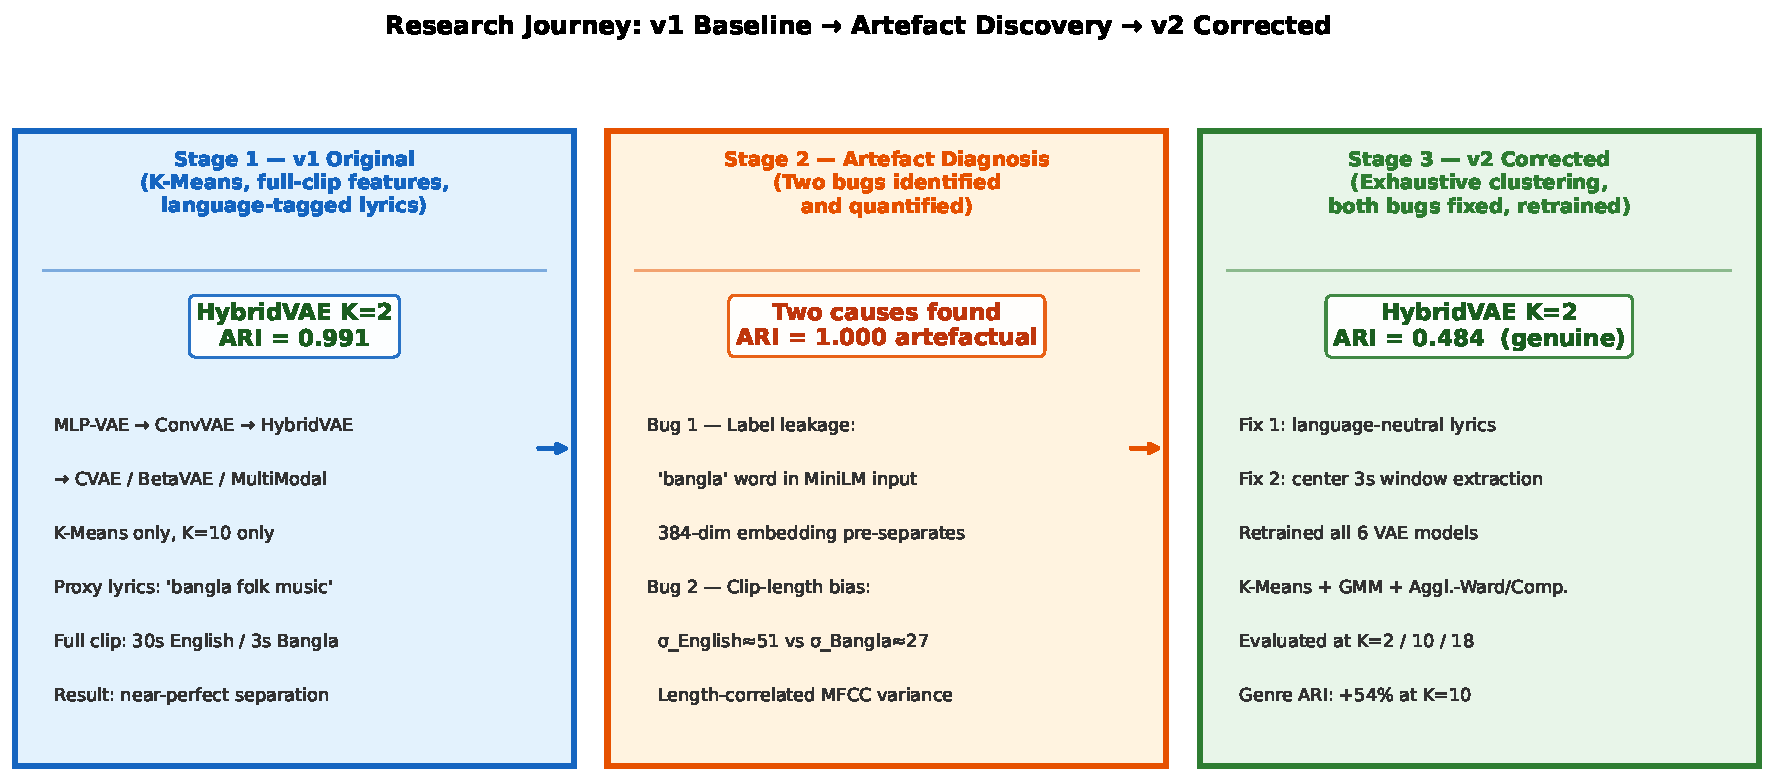
\includegraphics[width=\linewidth]{fig_v3_journey}
\caption{The three-stage research journey: v1 baseline (ARI\,=\,0.991 claimed) $\to$
artefact diagnosis (two bugs identified) $\to$ v2 corrected (genuine ARI\,=\,0.484).
Each panel summarises the key methods, features, and findings of that stage.}
\label{fig:journey}
\end{figure}

% ============================================================
\section{Related Work}
% ============================================================

\paragraph{Variational Autoencoders.}
Kingma and Welling~\cite{kingma2013auto} introduced VAEs via the evidence lower bound
(ELBO). Higgins et al.~\cite{higgins2017betavae} proposed $\beta$-VAE for disentangled
representations. Conditional VAEs~\cite{sohn2015learning} condition encoder and decoder
on auxiliary labels for class-conditional generation.

\paragraph{Music Representation Learning.}
MusicVAE~\cite{roberts2018hierarchical} demonstrated hierarchical latent representations
for symbolic music. Autoencoder approaches have been applied to instrument
recognition~\cite{choi2016automatic} and genre classification~\cite{dong2018convolutional}.

\paragraph{Multilingual Audio Understanding.}
wav2vec~\cite{baevski2020wav2vec} and CLAP~\cite{elizalde2022clap} provide cross-lingual
audio representations. Multilingual sentence transformers~\cite{reimers2019sentence}
bridge English and Bangla in a shared 384-dim semantic space.

\paragraph{Music Clustering.}
Tzanetakis and Cook~\cite{tzanetakis2002musical} established MFCC-based genre
classification as a benchmark. Levy and Sandler~\cite{levy2006music} applied
agglomerative clustering to audio similarity. To our knowledge, this is the first work
applying multi-modal VAEs to English--Bangla music clustering.

% ============================================================
\section{Shared Methodology}
\label{sec:method}
% ============================================================

\subsection{Dataset}

\begin{table}[H]
\centering
\caption{Dataset composition (identical across v1 and v2).}
\label{tab:dataset}
\small
\begin{tabular}{llrrr}
\toprule
\textbf{Source} & \textbf{Language} & \textbf{Tracks} & \textbf{Clip Length} & \textbf{Genres} \\
\midrule
GTZAN & English & 1,000 & 30 sec & 10 (blues, classical, country, \ldots) \\
MagnaTagATune & English & 9,000 & 29 sec & multi-tag (untagged in labeled eval) \\
BanglaBeats & Bangla & 10,020 & 3 sec & 8 (Adhunik, Folk, Hip-Hop, Indie, \ldots) \\
\midrule
\textbf{Total} & Both & \textbf{20,020} & --- & 18 labeled classes \\
\bottomrule
\end{tabular}
\end{table}

\subsection{Feature Extraction}

\textbf{MFCC Features (Easy Task):} 20 mel-frequency cepstral coefficients, 2048-sample FFT,
512-sample hop. Mean$+$std pooling yields 40-dim per track.

\textbf{Mel-Spectrogram Features (Medium/Hard Tasks):} 128-band log-mel spectrograms,
dB scale. Mean$+$std pooling yields 256-dim.

\textbf{Lyrics Embeddings:} Proxy English descriptions per genre, encoded by
\texttt{paraphrase-multilingual-MiniLM-L12-v2}~\cite{reimers2019sentence} to 384-dim.
\emph{Critical difference}: v1 used language-tagged descriptions;
v2 uses language-neutral descriptions (see Section~\ref{sec:stage2}).

\textbf{Combined Features (Hard Task, v2):} MFCC (20) + Chroma (12) + Spectral Contrast (7) +
Tonnetz (6), mean$+$std $=$ 90-dim, re-extracted from center 3\,s window of every clip.

\subsection{Model Architectures}

\paragraph{Task 1 --- MLP-VAE (Easy, BasicVAE).}
Encoder $[40\!\to\!512\!\to\!256]$, decoder $[32\!\to\!256\!\to\!512\!\to\!40]$,
$d_z\!=\!32$. Standard ELBO loss:
$\mathcal{L} = -\mathbb{E}[\log p(x|z)] + \mathrm{KL}[q(z|x) \| p(z)]$.

\paragraph{Task 2a --- ConvVAE (Medium).}
1D convolutional encoder on 256-dim mel features:
$[256 \to \mathrm{Conv}(64) \to \mathrm{Conv}(128) \to \mathrm{FC}(256) \to \mu, \sigma^2]$,
symmetric decoder.

\paragraph{Task 2b --- HybridVAE (Medium).}
256-dim mel $+$ 384-dim lyrics concatenated to 640-dim, then MLP-VAE ($d_z\!=\!32$,
hidden: $[512, 256]$). Early fusion enables joint acoustic--semantic encoding.

\paragraph{Task 3a --- MultiModalVAE (Hard).}
Separate encoders for audio and lyrics; fused at latent level before $\mu$/$\sigma^2$
projection. Reconstruction loss on audio only.

\paragraph{Task 3b --- CVAE (Hard).}
v1: language-only $c \in \mathbb{R}^{2}$. v2: language+genre one-hot $c \in \mathbb{R}^{22}$
concatenated to encoder and decoder: $q(z|x,c)$ and $p(x|z,c)$.

\paragraph{Task 3c --- Beta-VAE (Hard).}
MLP-VAE on combined features; $\beta$ controls KL regularisation strength.
$\beta\!=\!1$ confirmed optimal by grid search.

\subsection{Training Details}

Adam ($lr\!=\!10^{-3}$, $\beta_1\!=\!0.9$), batch 64, CPU.
Epochs: 100 (Easy), 80 (Medium), 60 (Hard).

\subsection{Why Three Values of $K$?}
\label{sec:why_k}

A key design decision is \emph{which $K$ to use} for evaluating unsupervised clustering.
We evaluate at three values, each motivated by the dataset structure:

\begin{figure}[H]
\centering
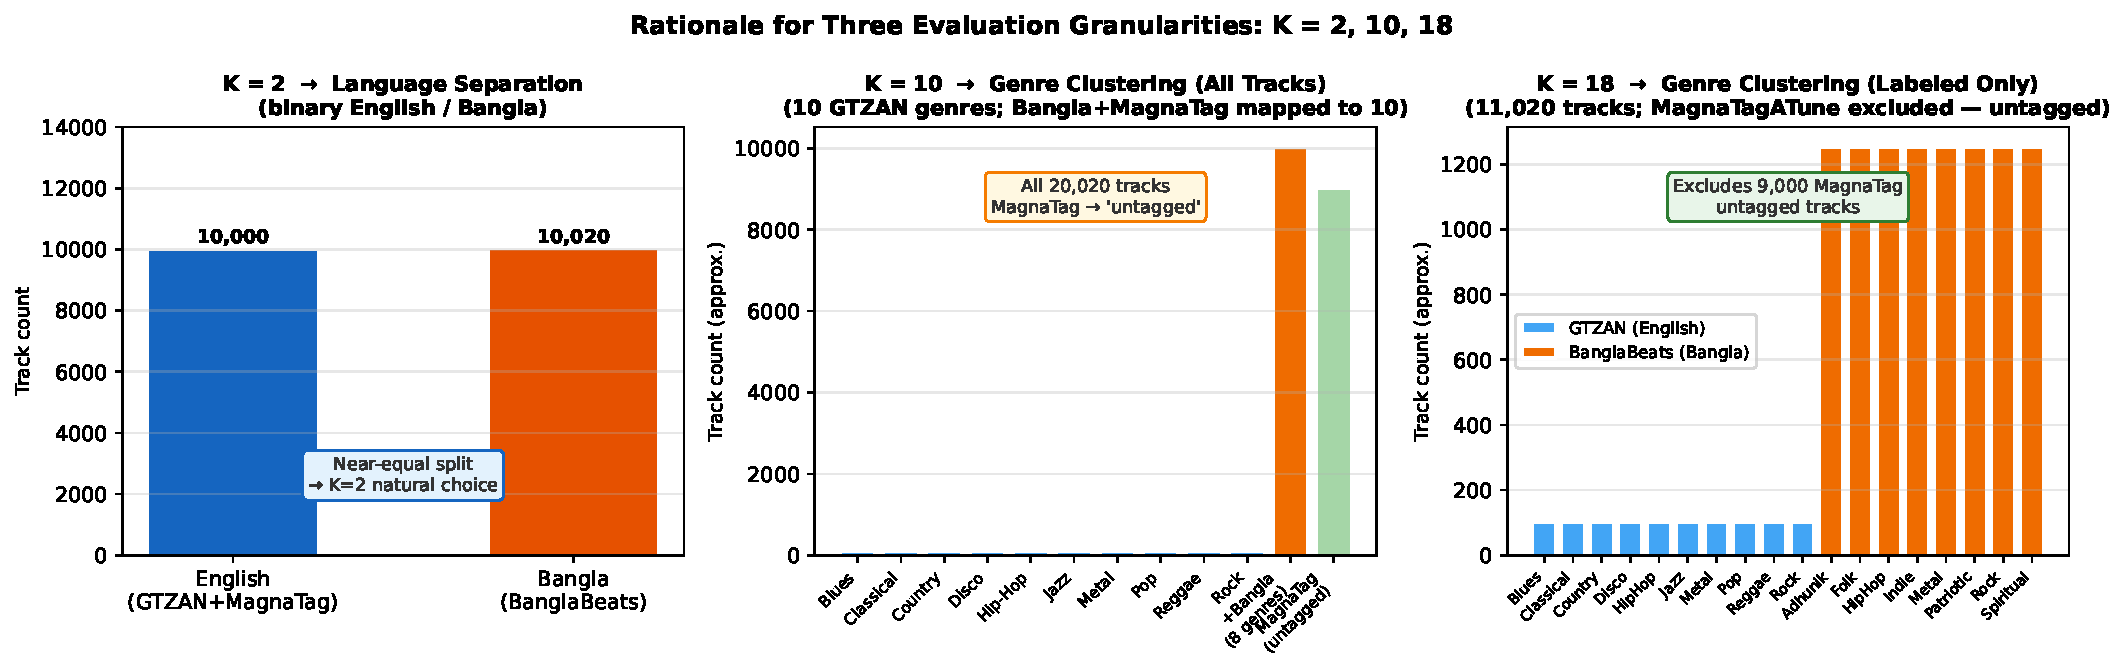
\includegraphics[width=\linewidth]{fig_v3_why_k}
\caption{Ground-truth label structure motivating three $K$ values.
Left: near-equal English/Bangla split (10,000 vs 10,020 tracks) motivates $K\!=\!2$.
Centre: 10 GTZAN genres + Bangla genres + MagnaTagATune mapped to 10 clusters.
Right: 18 distinct labeled genres (10 English + 8 Bangla) once MagnaTagATune's 9,000
untagged tracks are excluded.}
\label{fig:why_k}
\end{figure}

\begin{itemize}
    \item \textbf{$K\!=\!2$ (Language):} The dataset has a near-equal English/Bangla split
          (10,000 vs 10,020 tracks). This is the \emph{primary research question}: can VAEs
          spontaneously separate languages without any supervision? ARI at $K\!=\!2$ measures
          binary language alignment; Purity measures the dominant-language fraction per cluster.

    \item \textbf{$K\!=\!10$ (Genre-all):} GTZAN has exactly 10 genres. Evaluating all 20,020
          tracks at $K\!=\!10$ treats MagnaTagATune tracks as ``untagged'' (a single extra class
          diluting genre signal). This measures genre clustering ability on the full dataset and
          is directly comparable to the standard GTZAN benchmark.

    \item \textbf{$K\!=\!18$ (Genre-labeled):} Removing MagnaTagATune's 9,000 untagged tracks
          leaves 11,020 labeled tracks across 18 genres (10 GTZAN + 8 BanglaBeats). Setting
          $K\!=\!18$ matches the true number of genre classes, giving ARI its best chance---
          ARI is maximised when $K$ equals the number of ground-truth classes.
          This is the most \emph{informative} metric for genre alignment.
\end{itemize}

\noindent\textit{Why not just $K\!=\!10$?} ARI is $K$-sensitive: fewer clusters
($K\!=\!10$ vs 18 true classes) dilute label-alignment signal. Evaluating at all three
$K$ values gives a complete picture of what structure each model captures.

\subsection{Evaluation Metrics}

Six metrics: Silhouette Score (SS), Calinski-Harabasz Index (CHI),
Davies-Bouldin Index (DBI), Adjusted Rand Index (ARI), Normalized Mutual Information
(NMI), Cluster Purity. Three evaluation targets:
\begin{enumerate}
    \item \textbf{Language} ($K\!=\!2$): binary English/Bangla ground truth
    \item \textbf{Genre-all} ($K\!=\!10$): all 20,020 tracks; MagnaTagATune $\to$ ``untagged''
    \item \textbf{Genre-labeled} ($K\!=\!18$): 11,020 labeled tracks (GTZAN+BanglaBeats only)
\end{enumerate}

% ============================================================
\section{Stage 1 --- v1 Original Results}
\label{sec:stage1}
% ============================================================

Stage 1 (v1) used original feature extraction (full clip, language-tagged proxy lyrics)
and K-Means only. All results in this section are from the original v1 checkpoint files.

\begin{figure}[H]
\centering
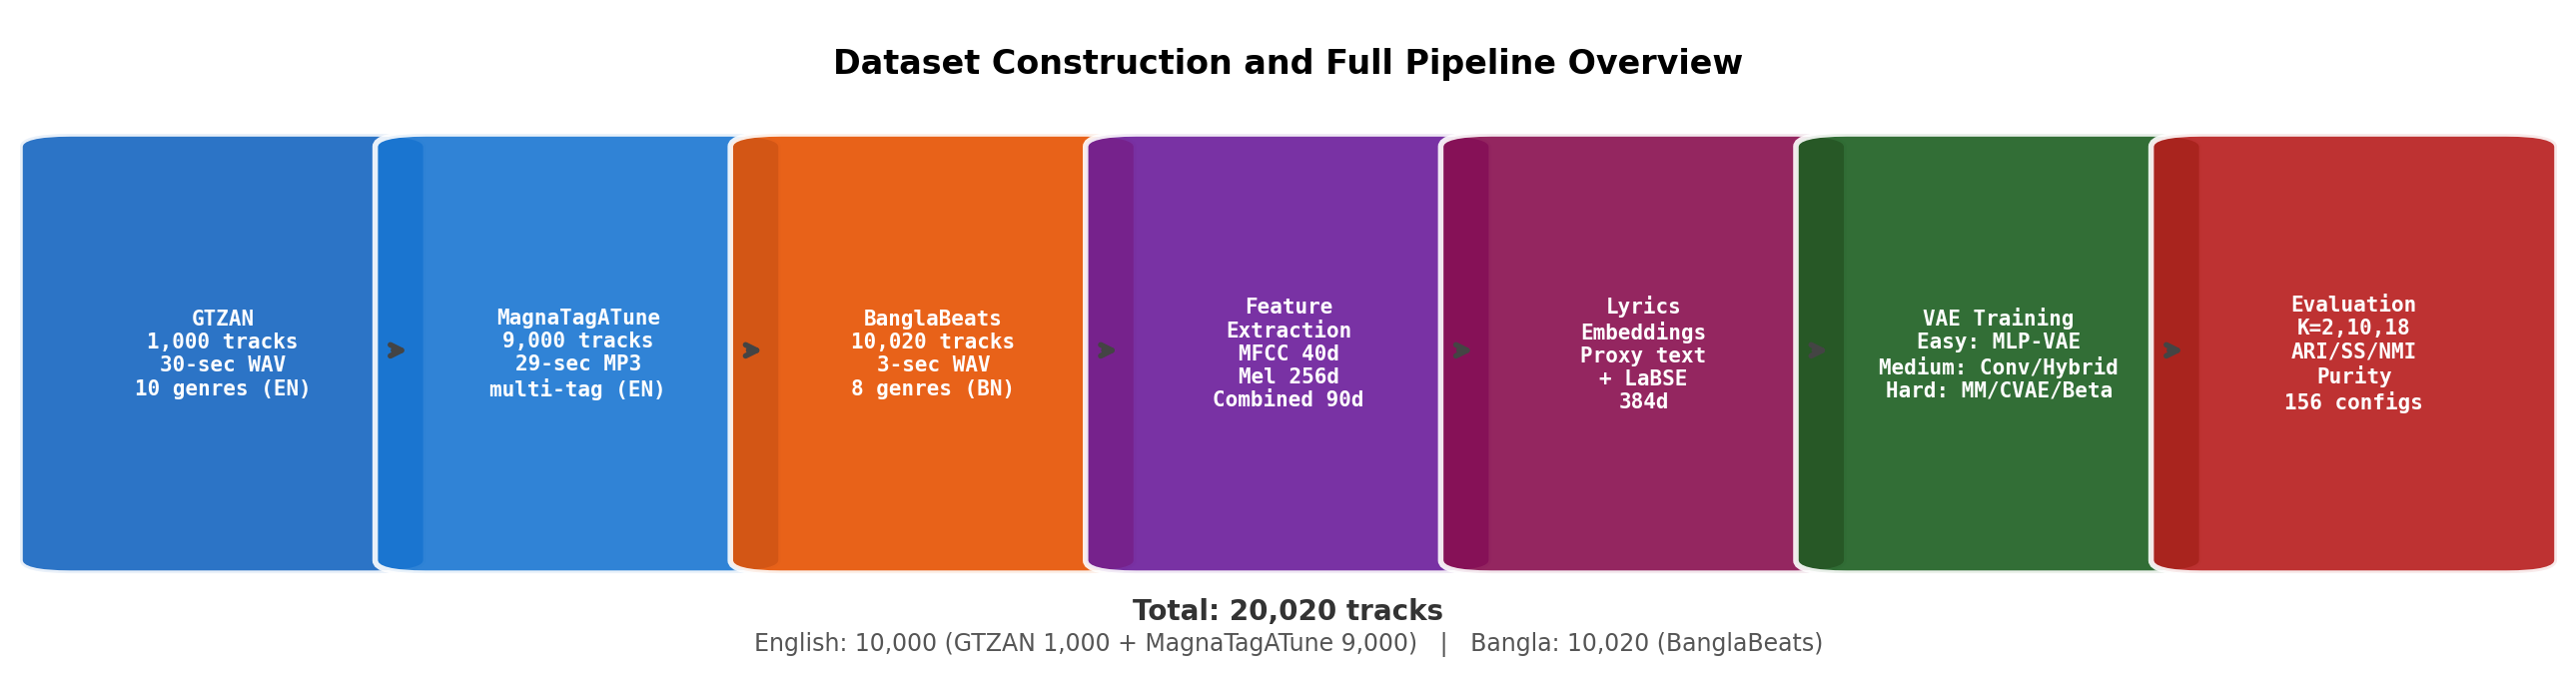
\includegraphics[width=0.85\linewidth]{dataset_pipeline}
\caption{Data preprocessing and VAE pipeline overview. Audio is loaded at 22,050\,Hz;
features extracted per-clip and normalised; VAE trained end-to-end on the full 20,020-track
dataset.}
\label{fig:pipeline}
\end{figure}

\begin{figure}[H]
\centering
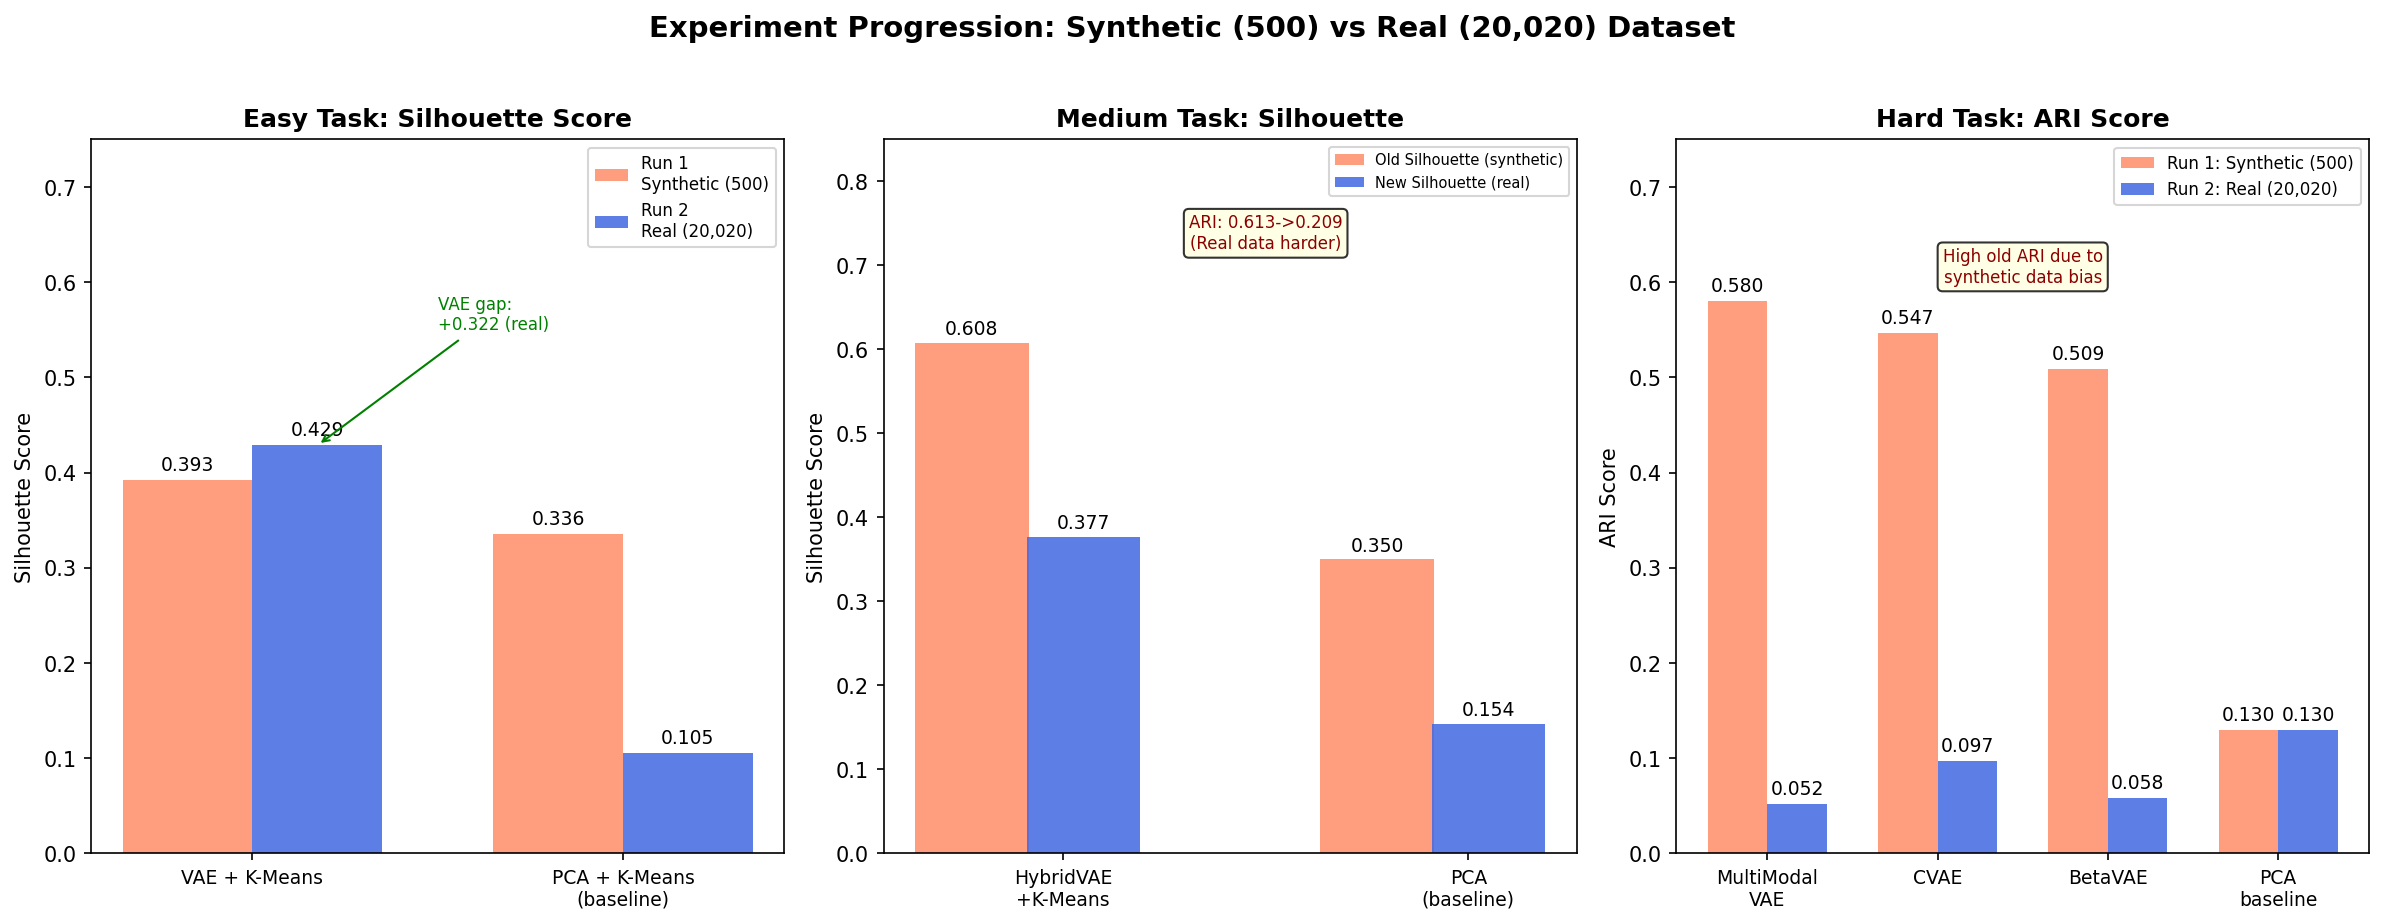
\includegraphics[width=0.85\linewidth]{progression_comparison}
\caption{Ablation: synthetic 500-sample vs.\ real 20,020-sample dataset.
VAE Silhouette: $0.393 \to 0.429$ (+9\%). PCA Silhouette: $0.336 \to 0.105$ ($-69\%$),
demonstrating VAE robustness to data diversity.}
\label{fig:progression}
\end{figure}

\begin{figure}[H]
\centering
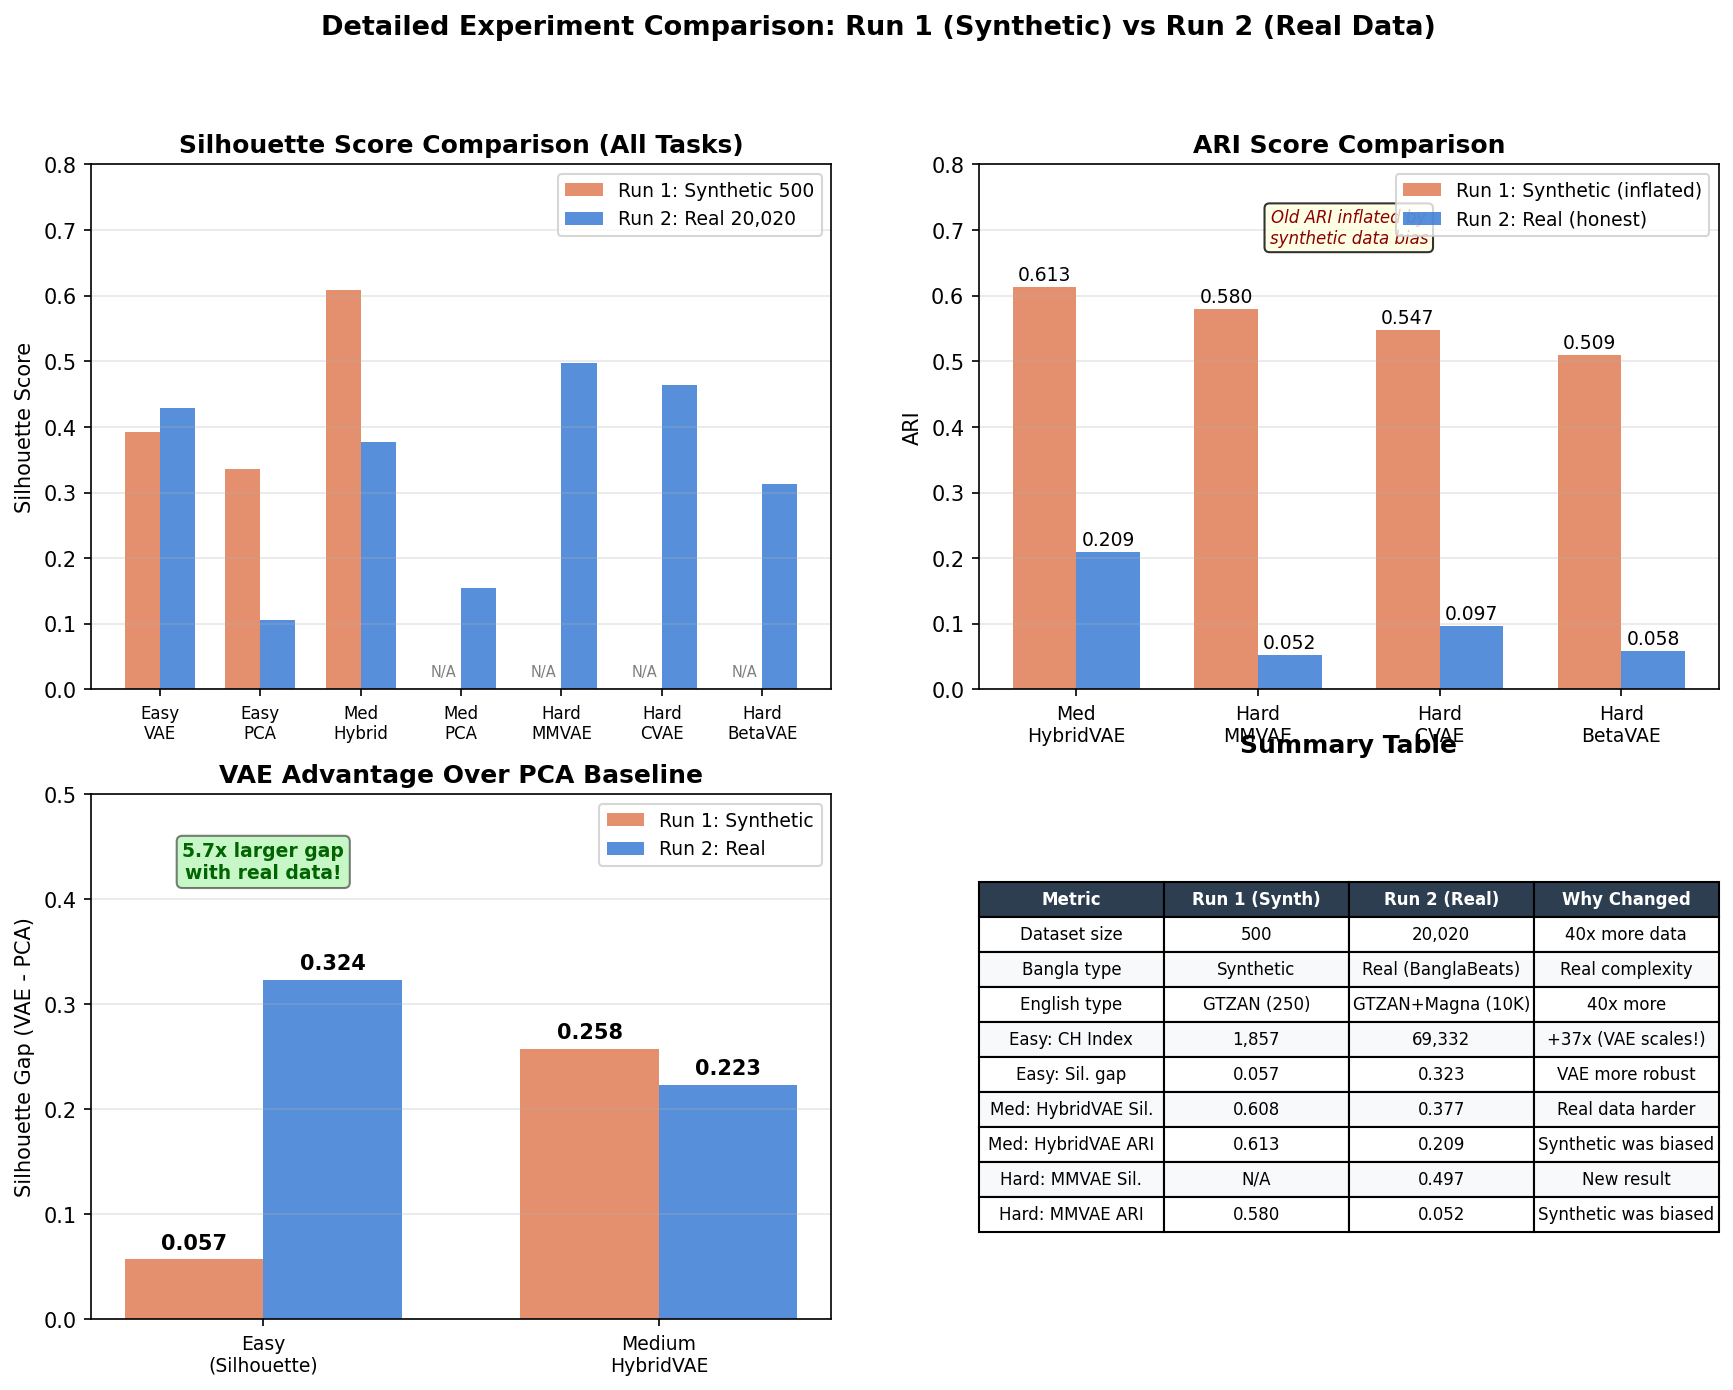
\includegraphics[width=\linewidth]{full_comparison}
\caption{Comprehensive comparison: SS and ARI for synthetic vs.\ real data, VAE vs.\
PCA gap across tasks. VAE representations are significantly more robust to scale.}
\label{fig:full_comparison}
\end{figure}

\subsection{v1 Easy Task: MLP-VAE on MFCC}

\begin{figure}[H]
\centering
\begin{subfigure}[b]{0.48\linewidth}
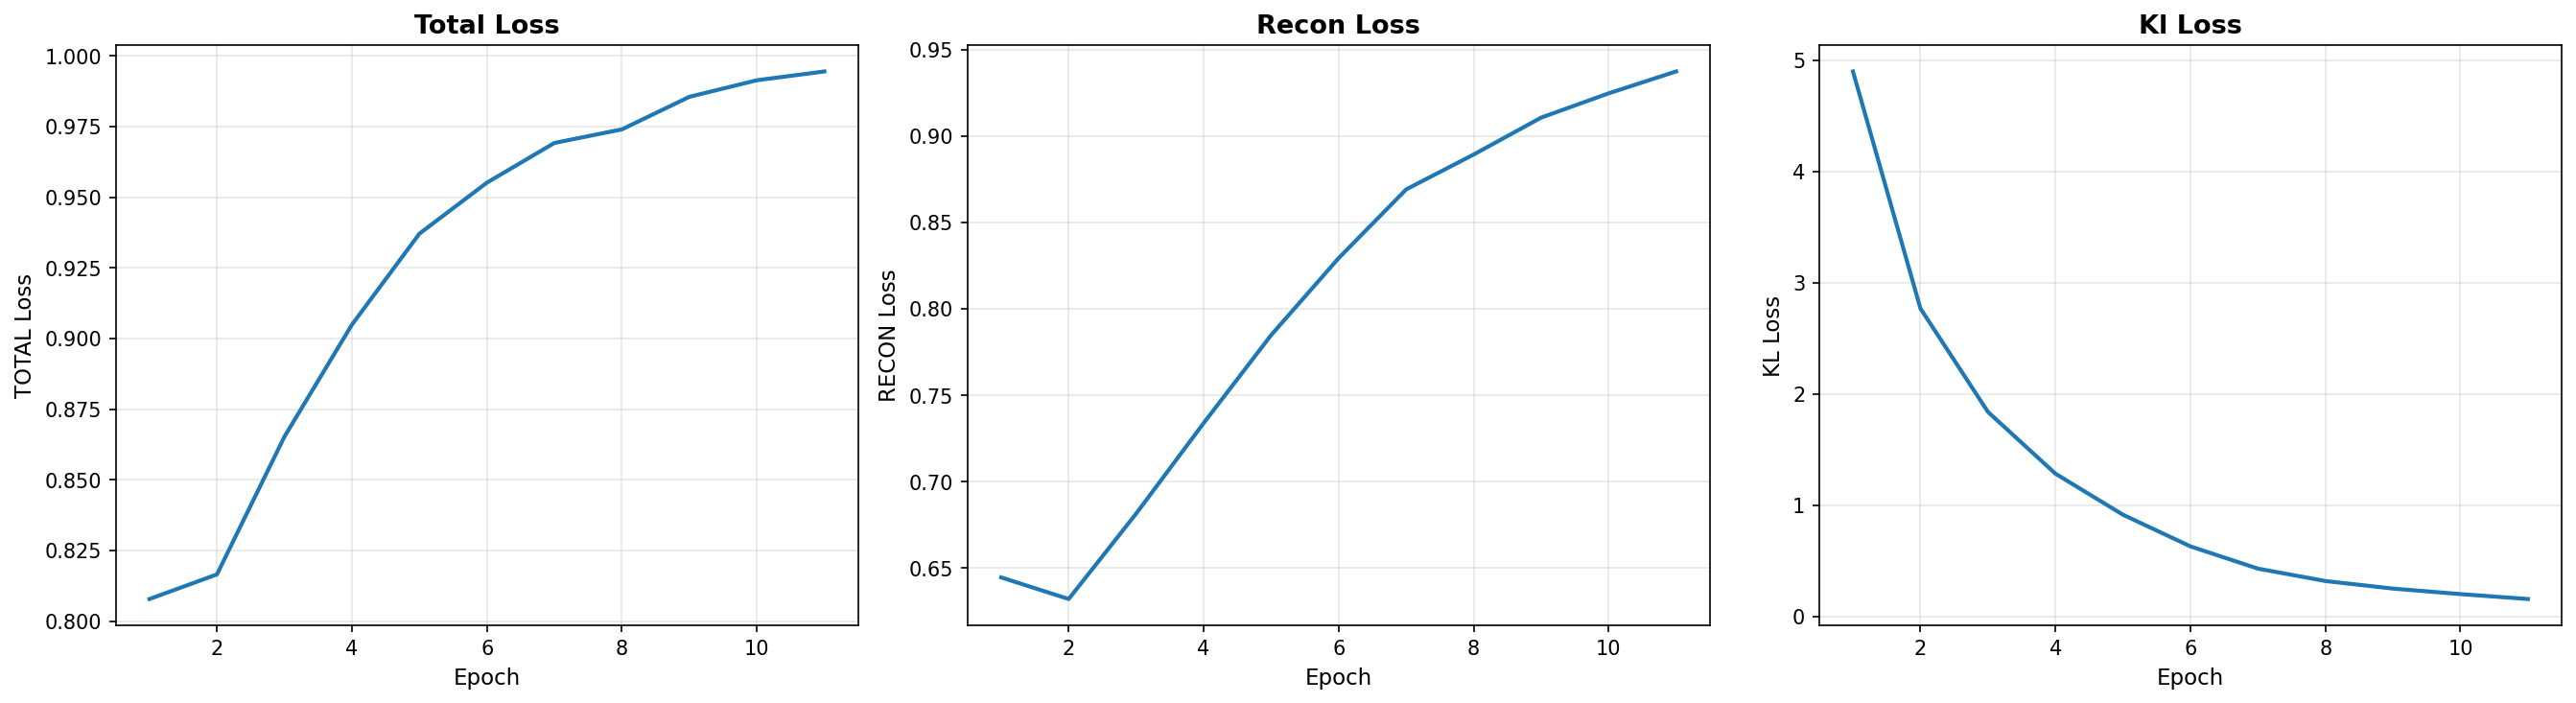
\includegraphics[width=\linewidth]{easy_training}
\caption{MLP-VAE training curves (100 epochs)}
\end{subfigure}
\hfill
\begin{subfigure}[b]{0.48\linewidth}
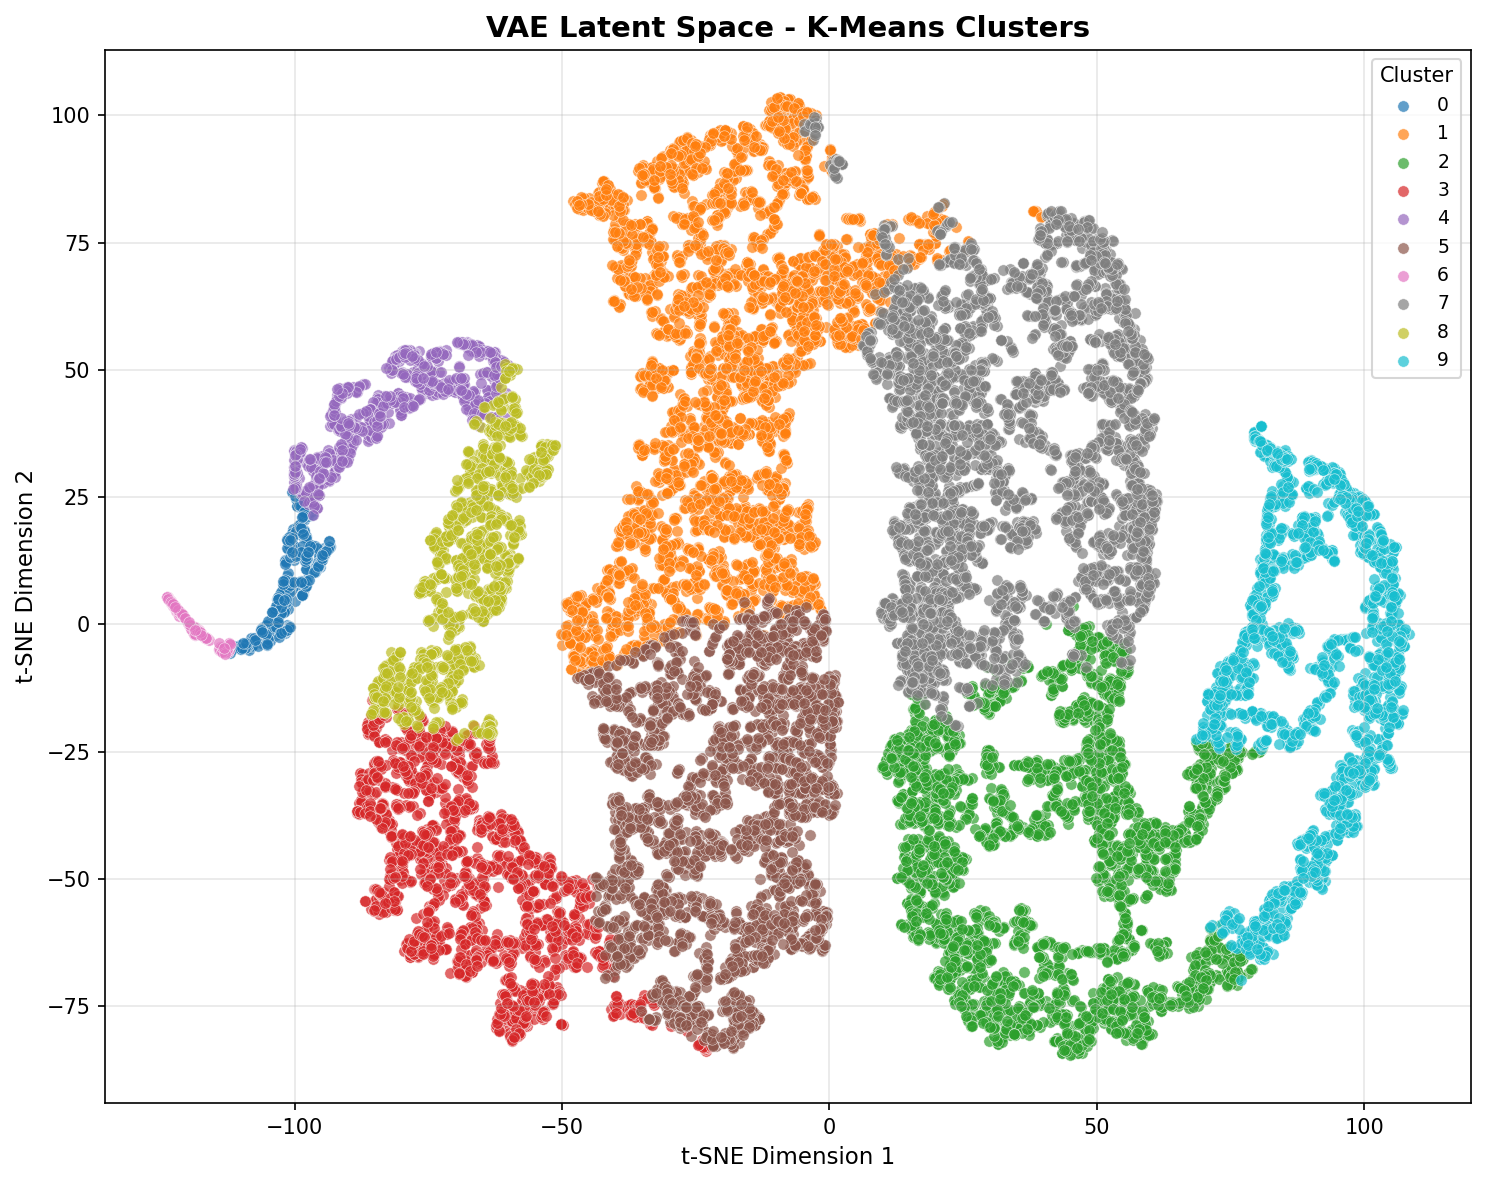
\includegraphics[width=\linewidth]{easy_tsne_kmeans}
\caption{t-SNE of VAE latent space ($K\!=\!10$ clusters)}
\end{subfigure}
\caption{v1 Easy Task: MLP-VAE training convergence and latent space cluster structure.}
\label{fig:v1_easy}
\end{figure}

\begin{figure}[H]
\centering
\begin{subfigure}[b]{0.48\linewidth}
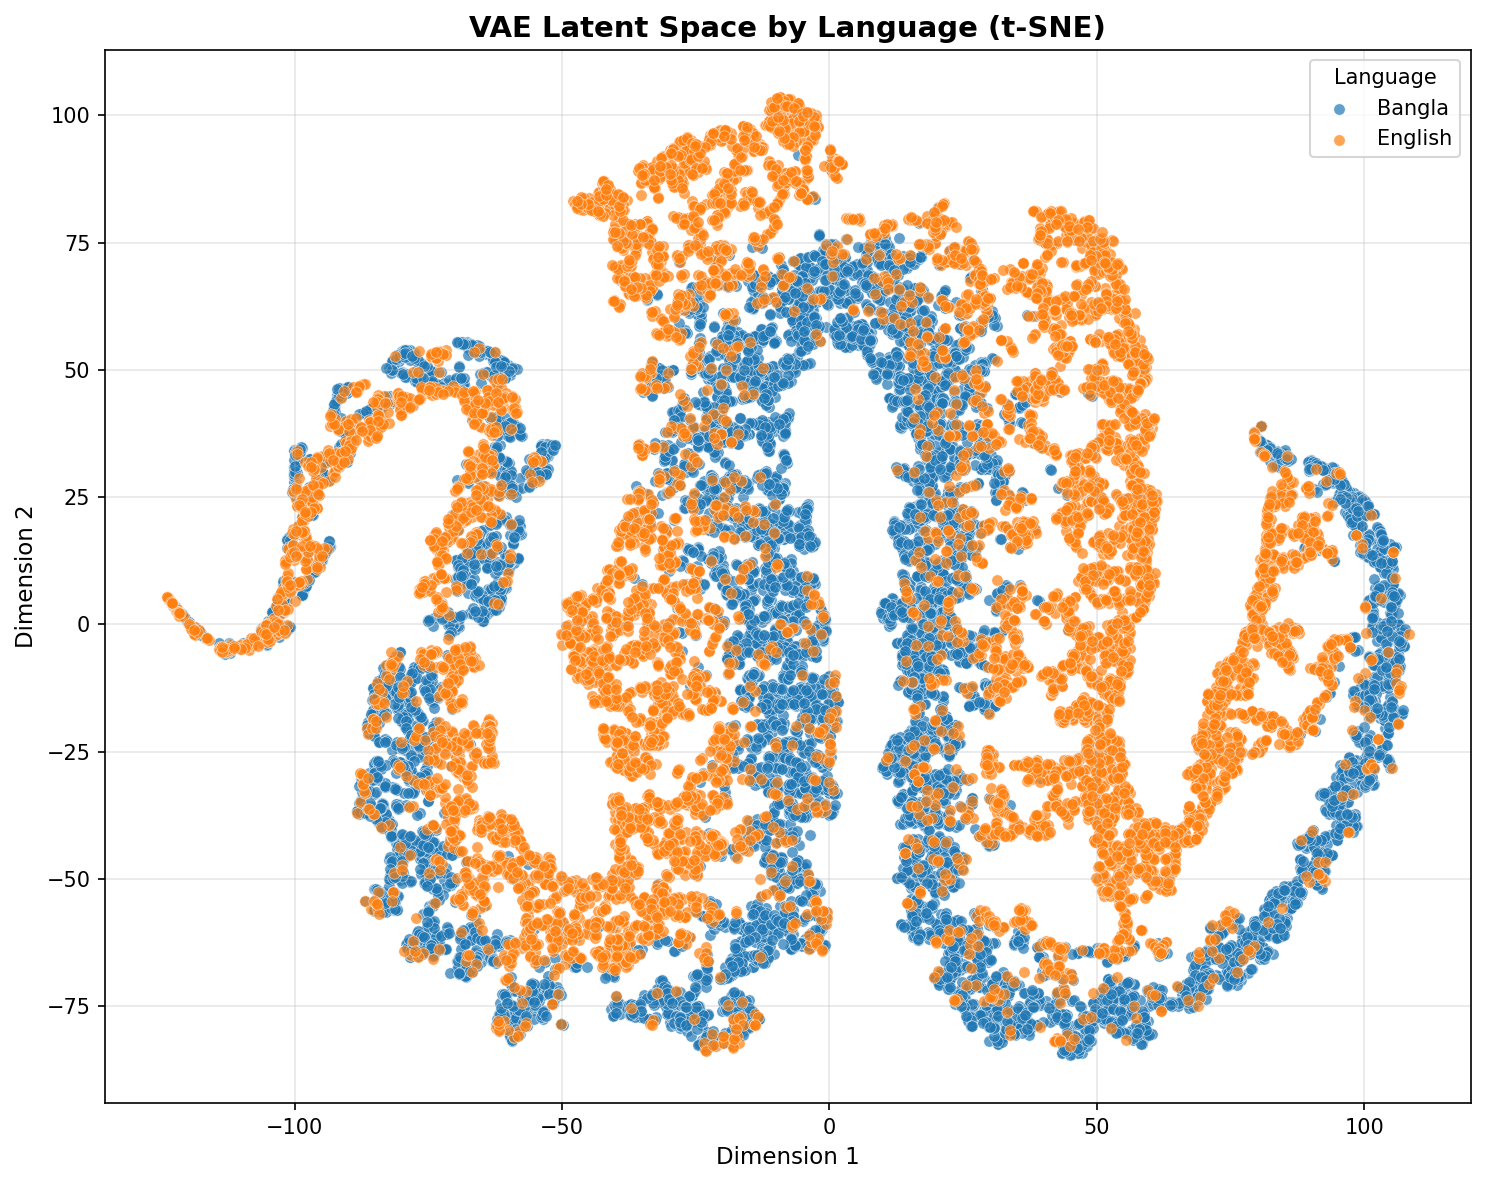
\includegraphics[width=\linewidth]{easy_tsne_language}
\caption{Easy VAE latent space by language}
\end{subfigure}
\hfill
\begin{subfigure}[b]{0.48\linewidth}
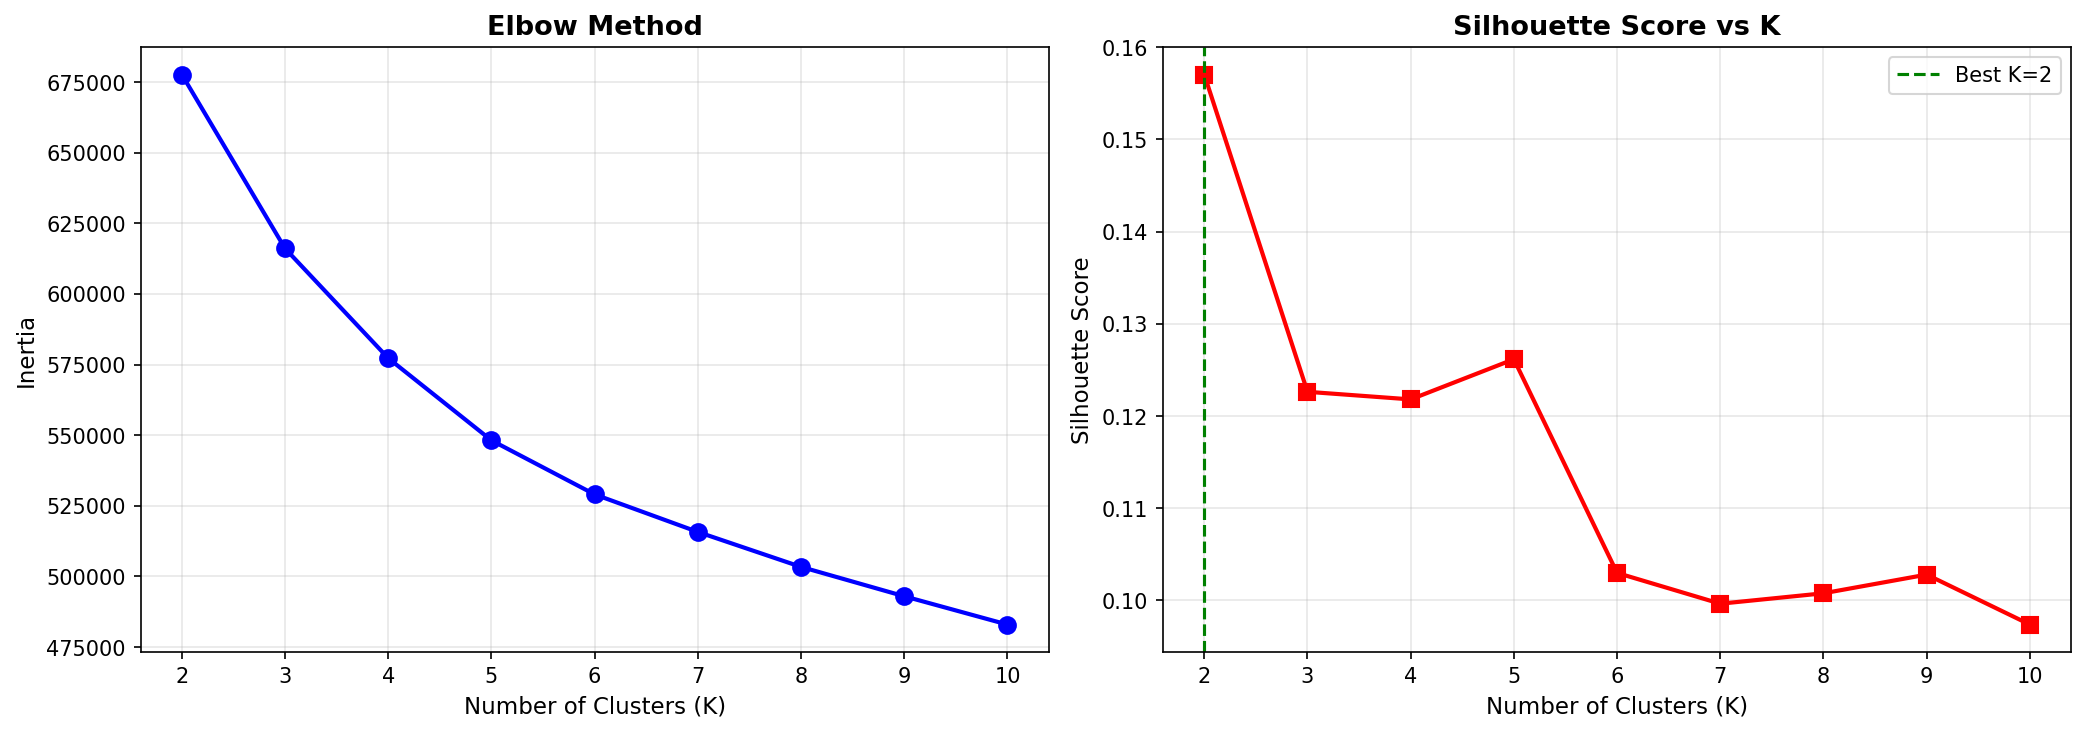
\includegraphics[width=\linewidth]{easy_elbow}
\caption{Elbow/Silhouette analysis}
\end{subfigure}
\caption{v1 Easy Task: MFCC features show partial language separation (clip-length bias
visible as two-cloud structure). Elbow around $K\!=\!8$--$10$ confirms $K\!=\!10$.}
\label{fig:v1_easy_lang}
\end{figure}

\subsection{v1 Medium Task: ConvVAE and HybridVAE}

\begin{figure}[H]
\centering
\begin{subfigure}[b]{0.48\linewidth}
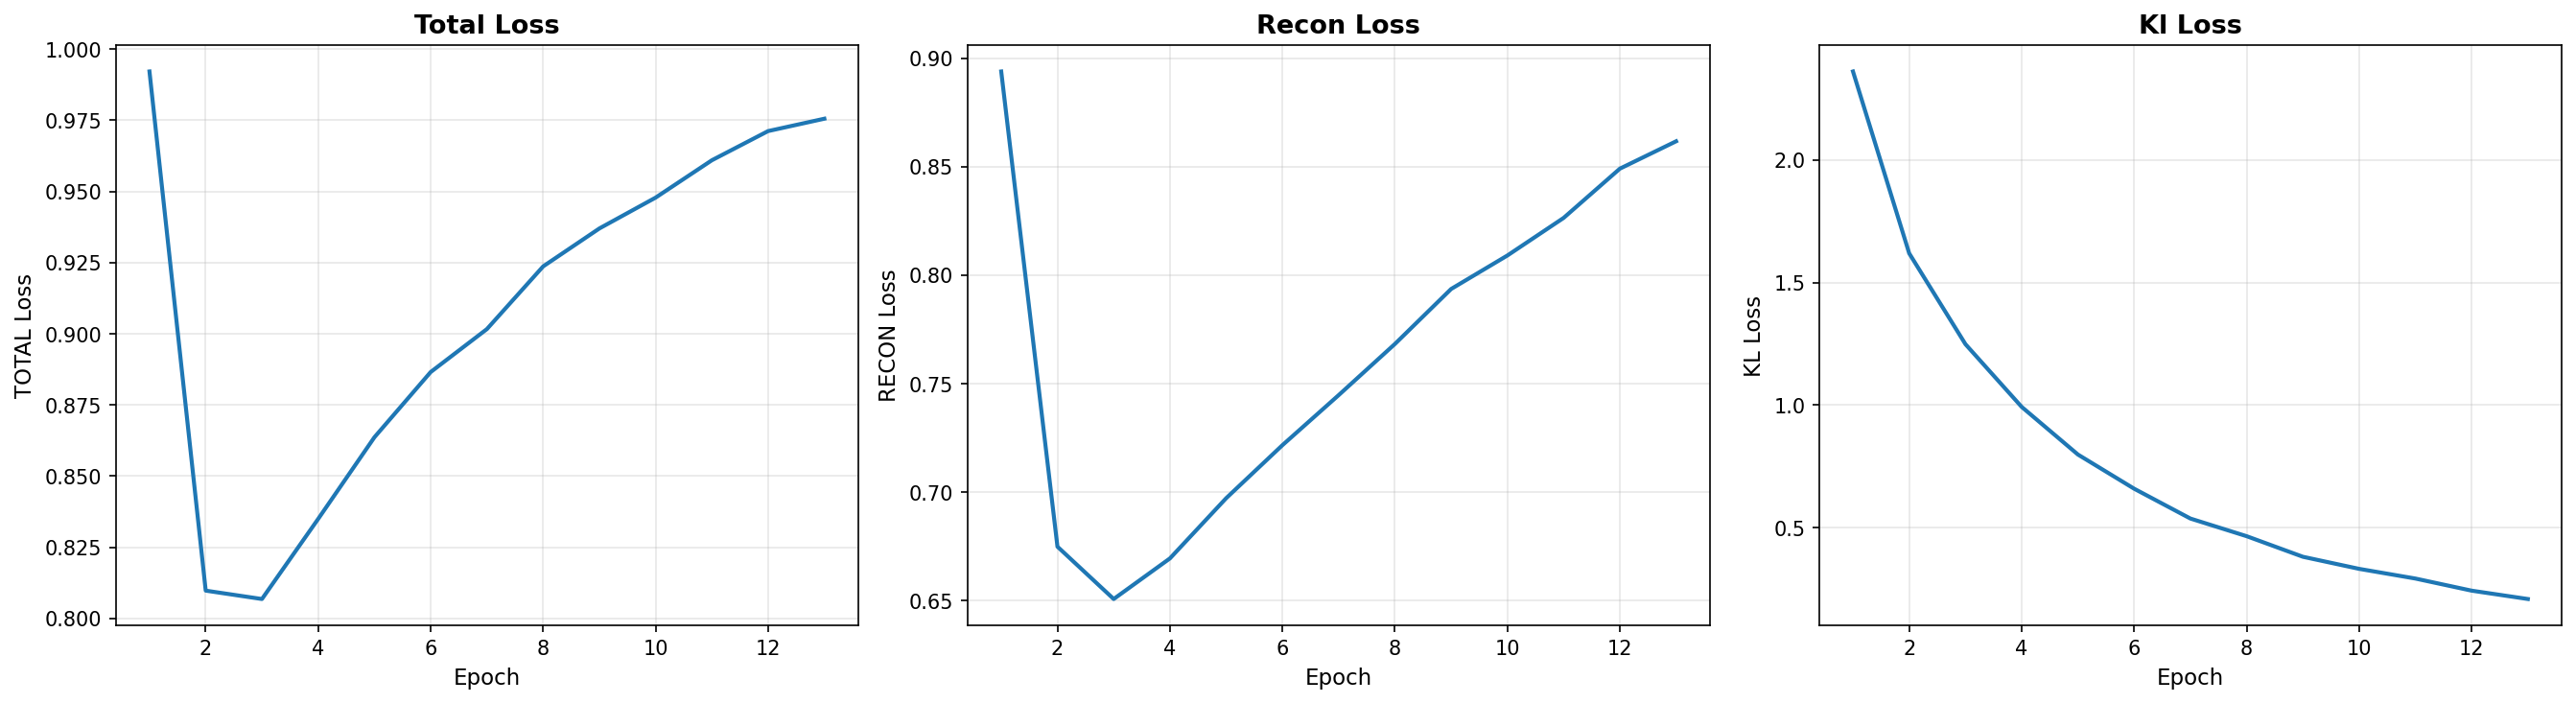
\includegraphics[width=\linewidth]{medium_conv_training}
\caption{ConvVAE training (80 epochs)}
\end{subfigure}
\hfill
\begin{subfigure}[b]{0.48\linewidth}
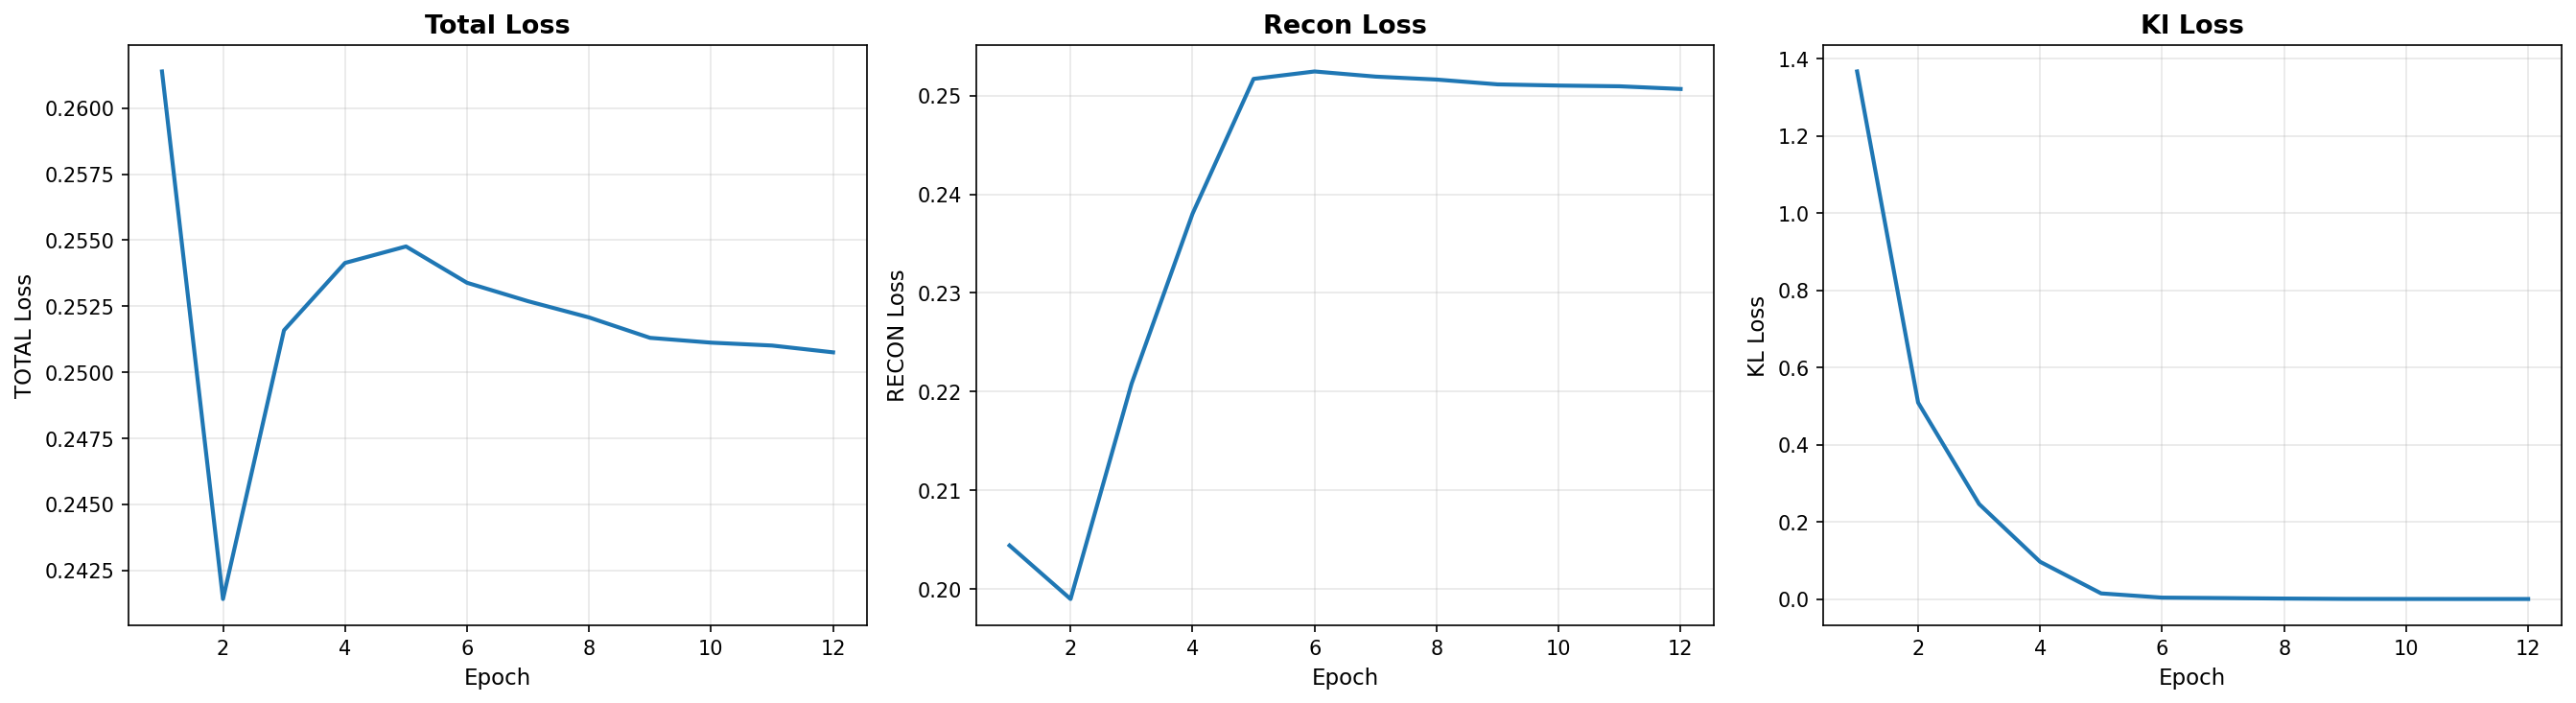
\includegraphics[width=\linewidth]{medium_hybrid_training}
\caption{HybridVAE training (80 epochs)}
\end{subfigure}
\caption{v1 Medium Task training curves. HybridVAE converges on 640-dim joint input.}
\label{fig:v1_medium_training}
\end{figure}

\begin{figure}[H]
\centering
\begin{subfigure}[b]{0.48\linewidth}
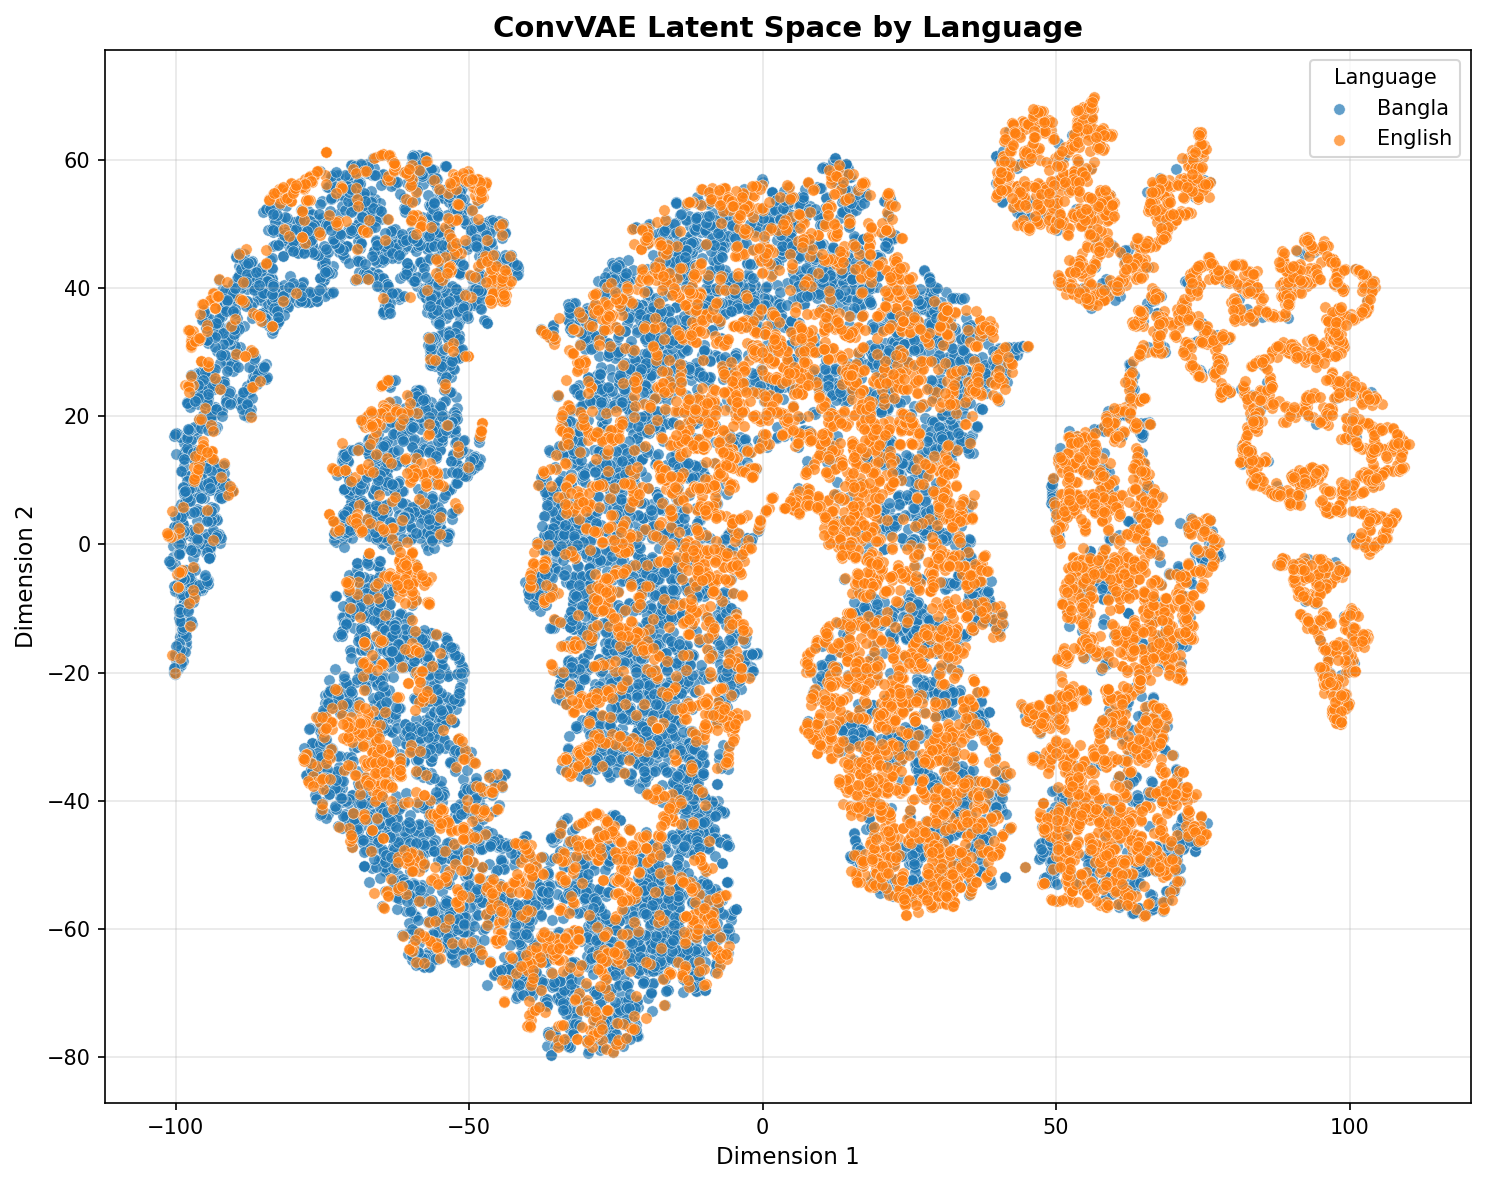
\includegraphics[width=\linewidth]{medium_conv_language}
\caption{ConvVAE latent space by language}
\end{subfigure}
\hfill
\begin{subfigure}[b]{0.48\linewidth}
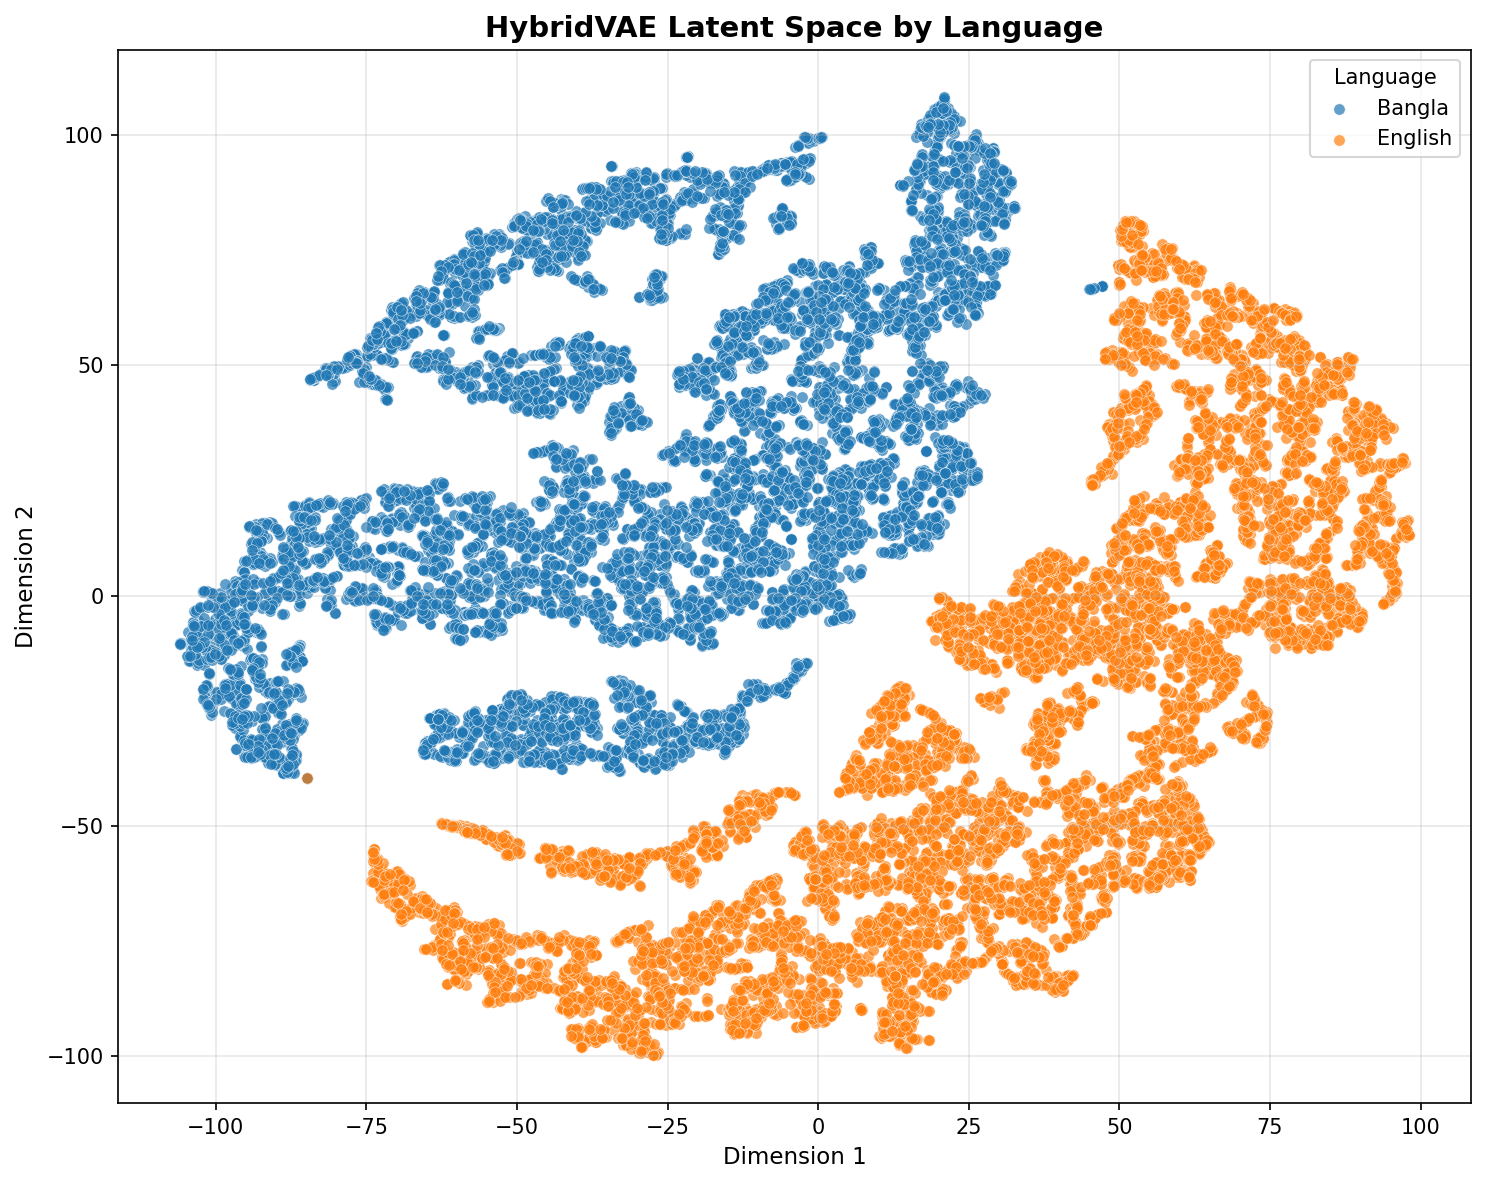
\includegraphics[width=\linewidth]{medium_hybrid_language}
\caption{HybridVAE latent space by language}
\end{subfigure}
\caption{v1 Medium Task: t-SNE by language. HybridVAE (right) shows dramatically clean
two-cluster separation driven by language-tagged proxy lyrics---the v1 artefact
(ARI\,=\,0.991, identified in Stage~2 as label leakage).}
\label{fig:v1_medium_lang}
\end{figure}

\begin{figure}[H]
\centering
\begin{subfigure}[b]{0.48\linewidth}
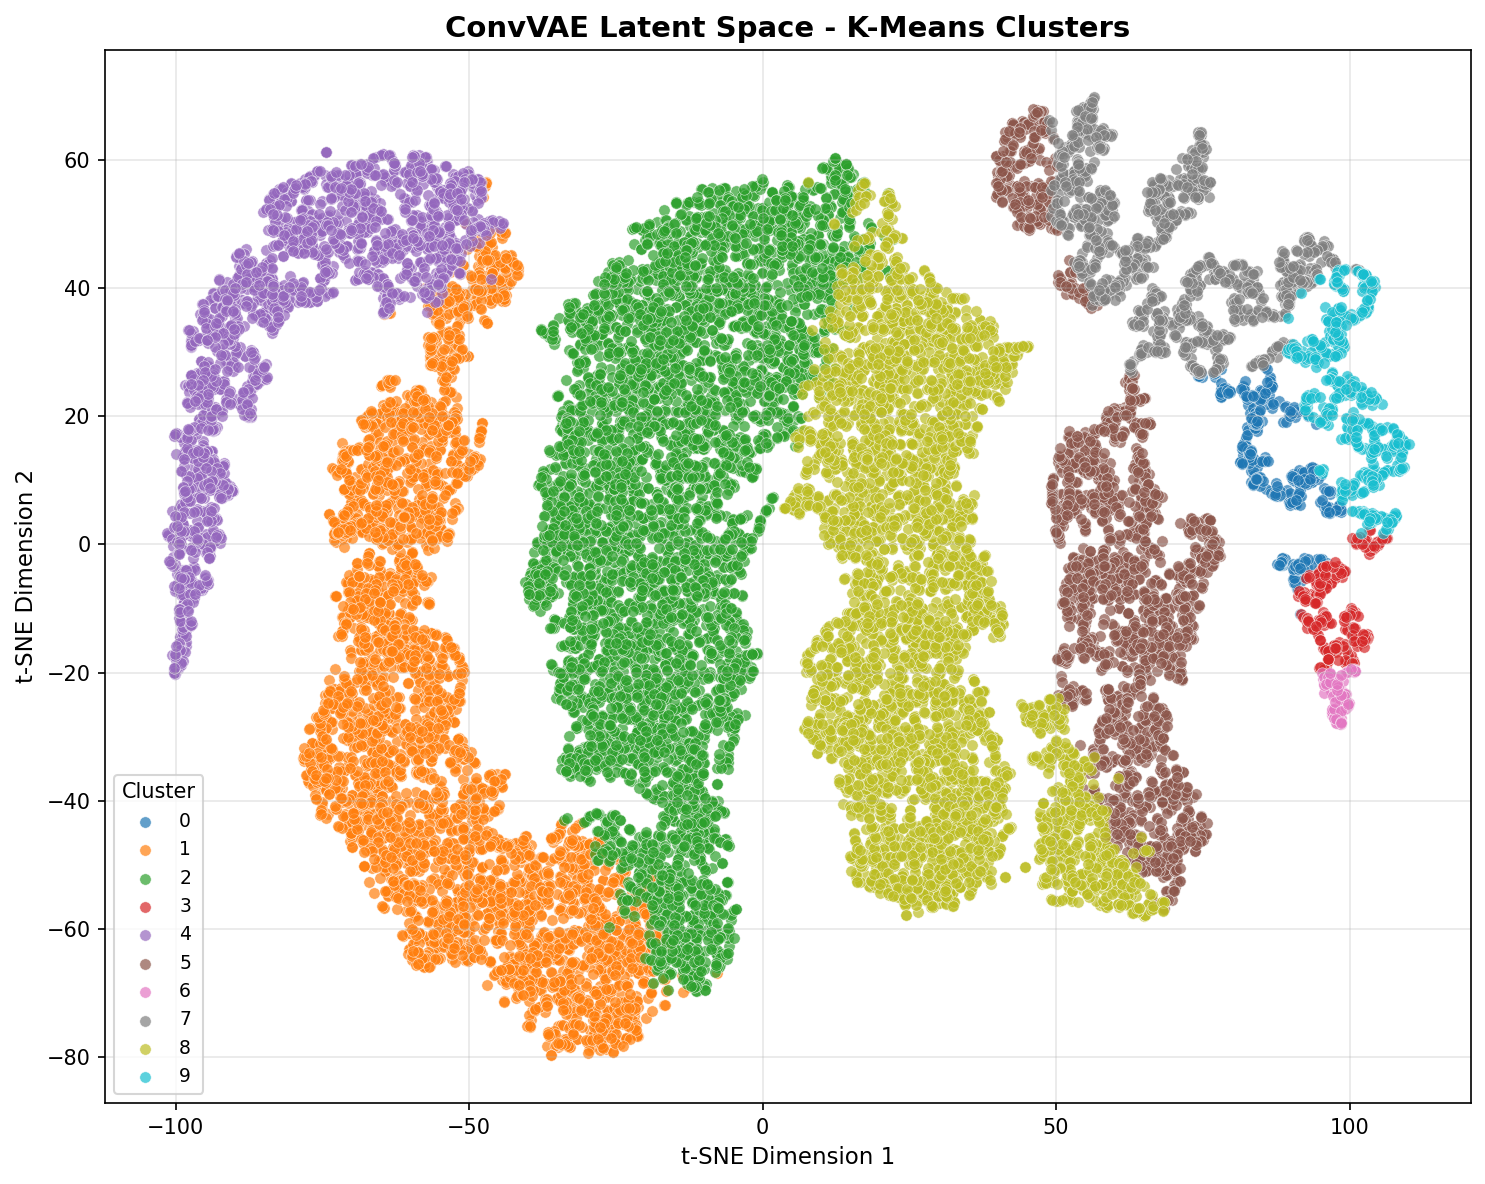
\includegraphics[width=\linewidth]{medium_tsne_kmeans}
\caption{ConvVAE/HybridVAE clusters ($K\!=\!10$)}
\end{subfigure}
\hfill
\begin{subfigure}[b]{0.48\linewidth}
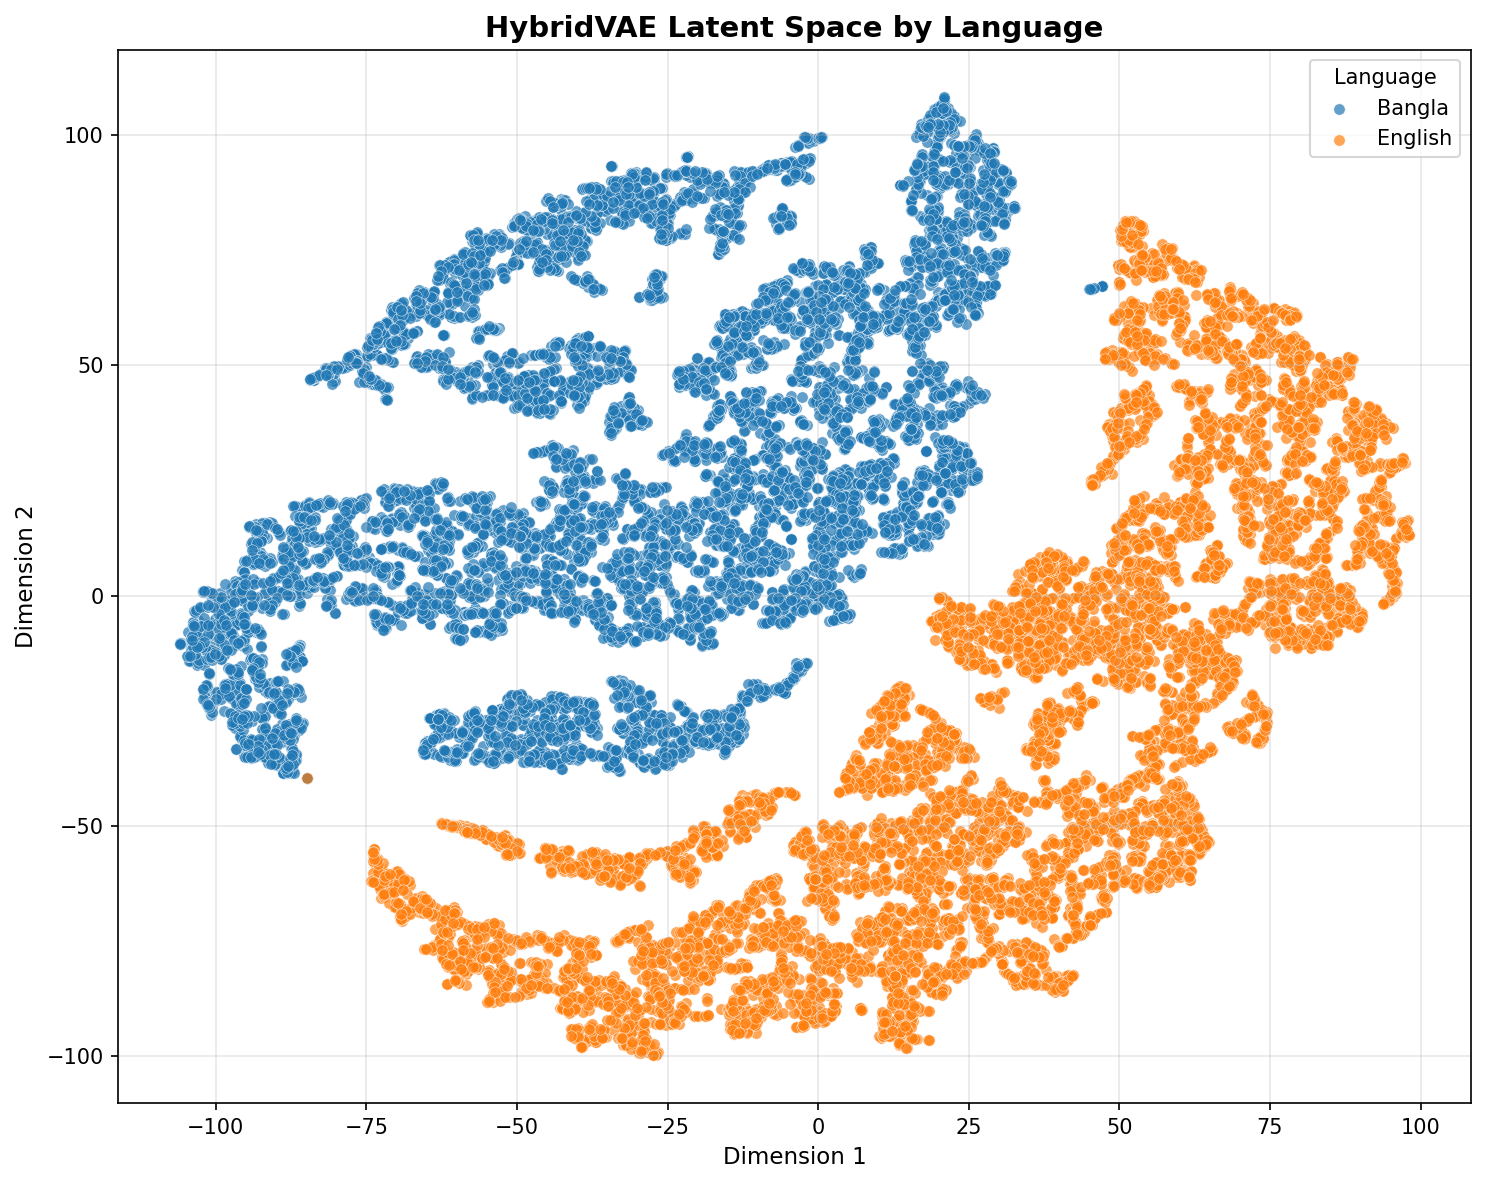
\includegraphics[width=\linewidth]{medium_tsne_language}
\caption{Medium t-SNE by language (both models)}
\end{subfigure}
\caption{v1 Medium Task: K-Means cluster structure and language separation.}
\label{fig:v1_medium_tsne}
\end{figure}

\subsection{v1 Hard Task: MultiModalVAE, CVAE, and Beta-VAE}

\begin{figure}[H]
\centering
\begin{subfigure}[b]{0.32\linewidth}
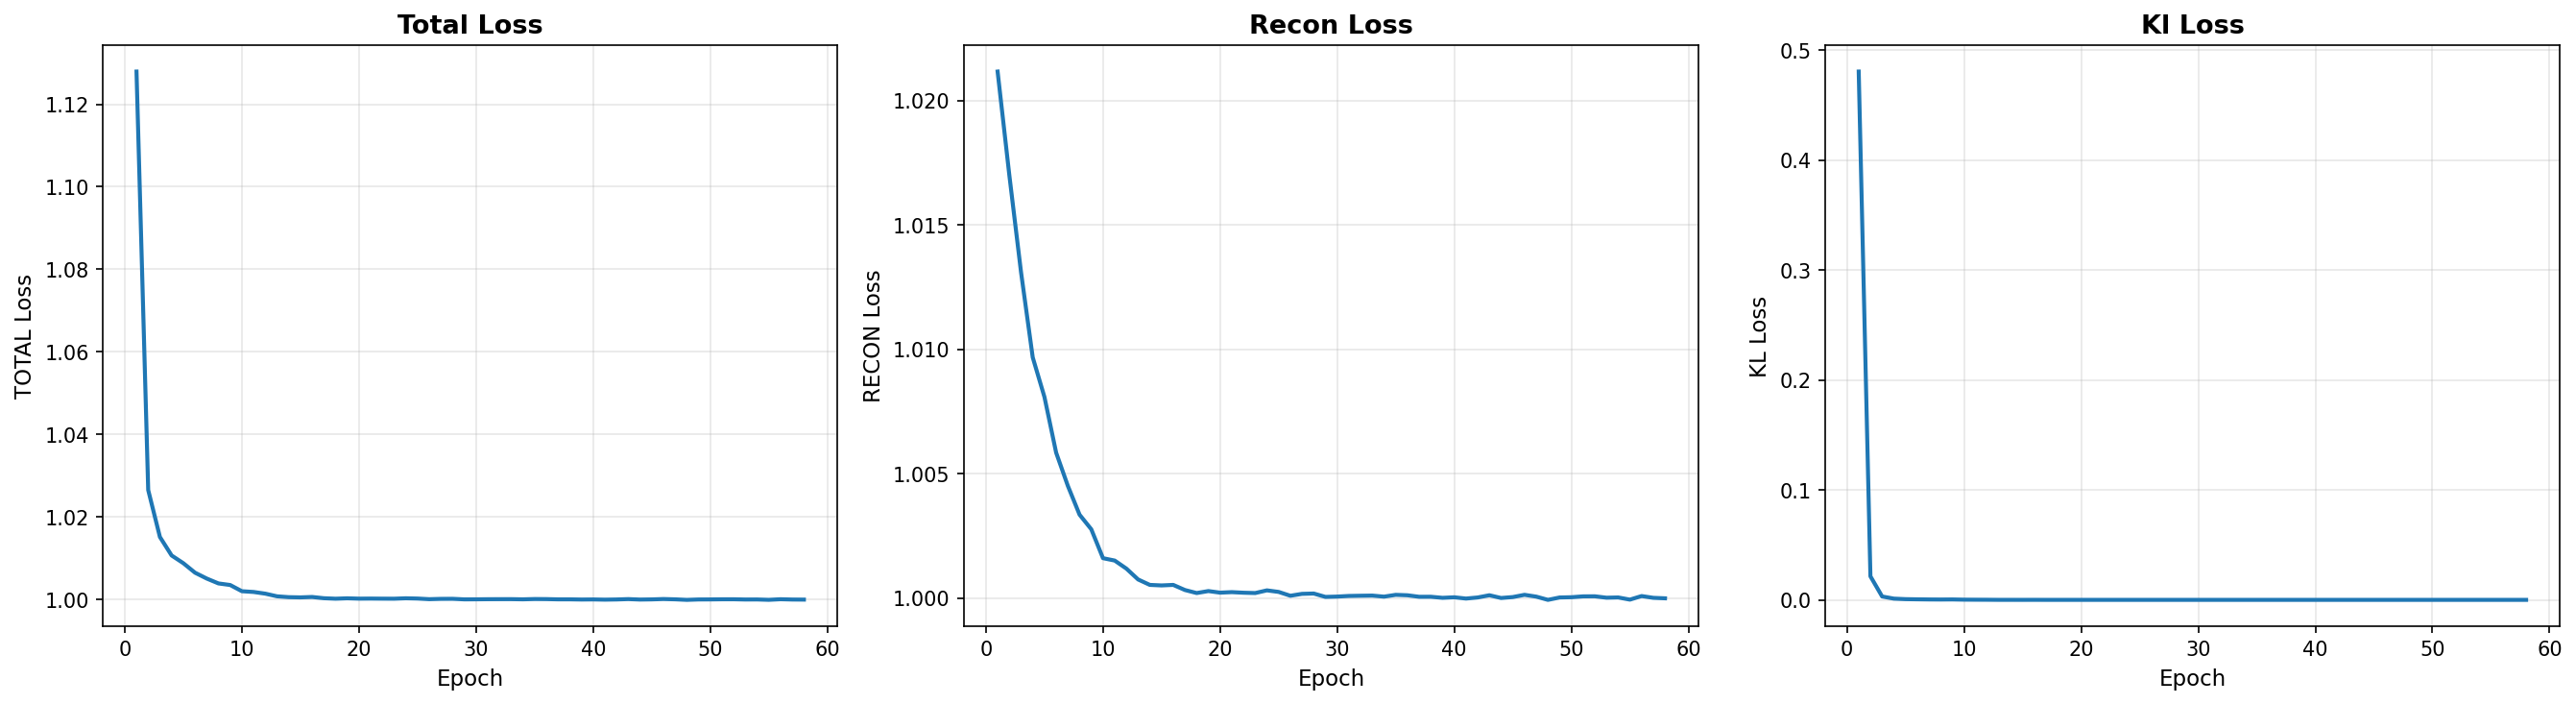
\includegraphics[width=\linewidth]{hard_beta_training}
\caption{BetaVAE ($\beta\!=\!1$) training}
\end{subfigure}
\hfill
\begin{subfigure}[b]{0.32\linewidth}
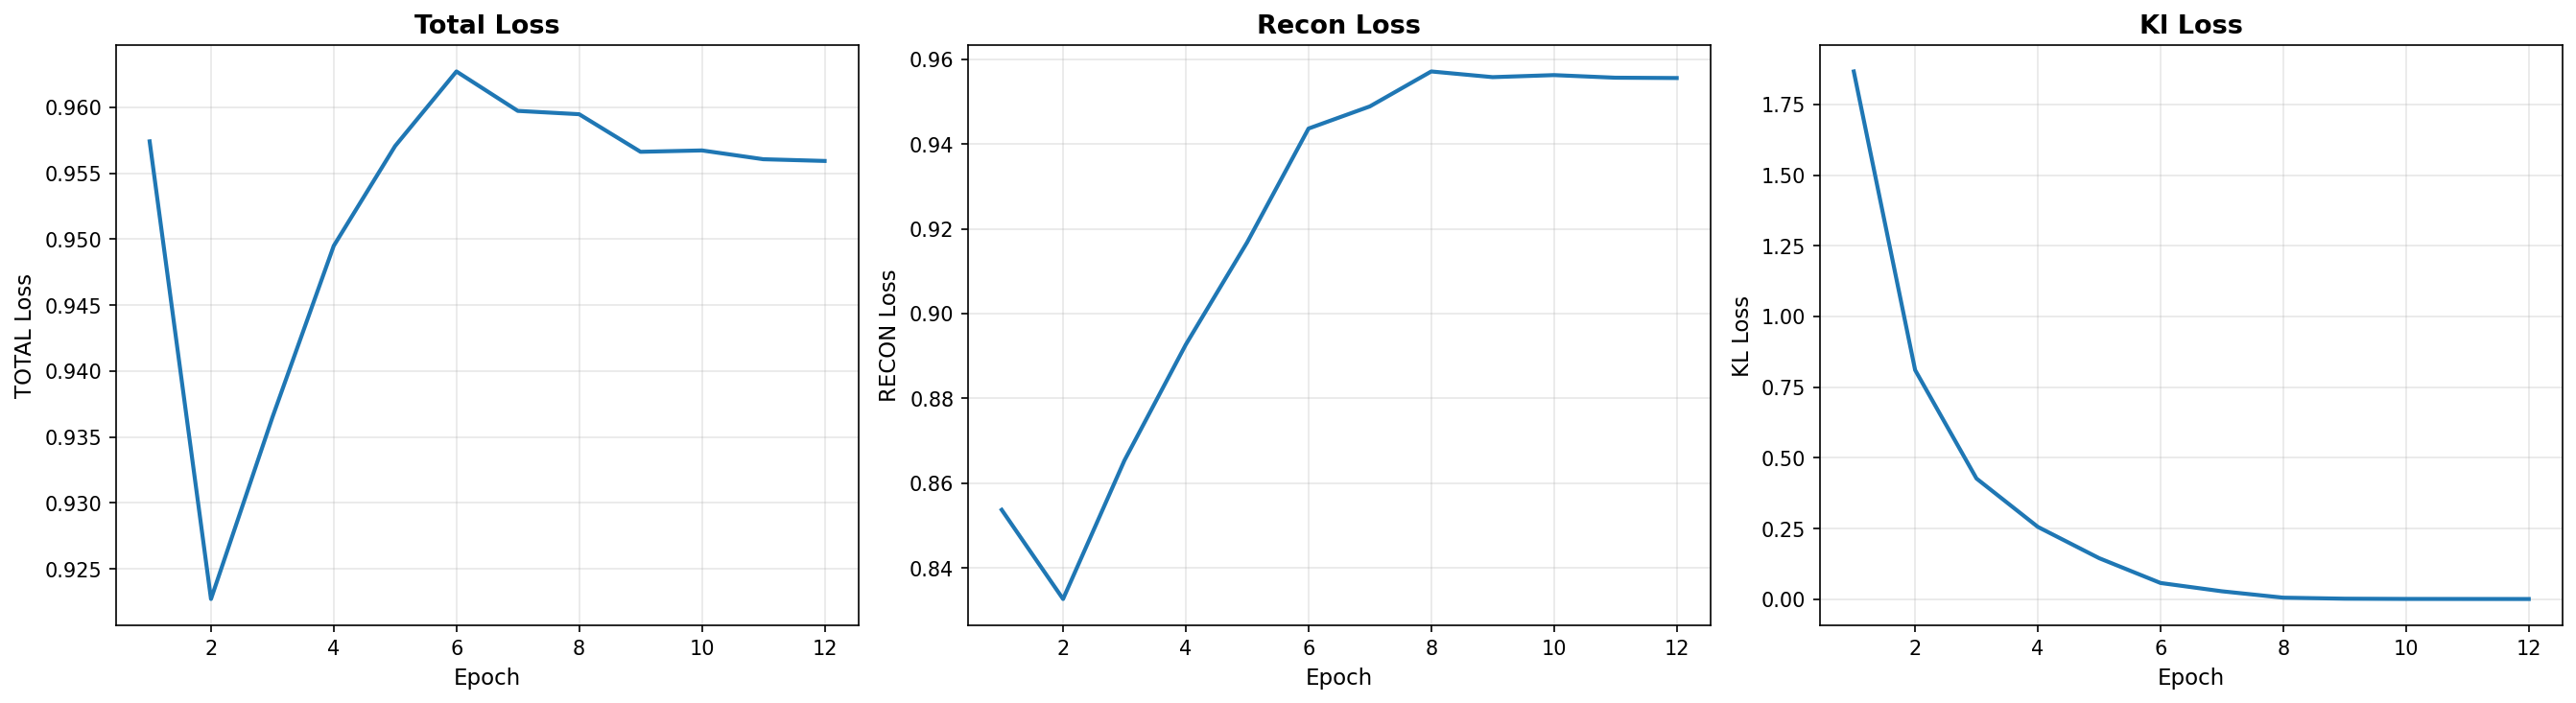
\includegraphics[width=\linewidth]{hard_cvae_training}
\caption{CVAE training}
\end{subfigure}
\hfill
\begin{subfigure}[b]{0.32\linewidth}
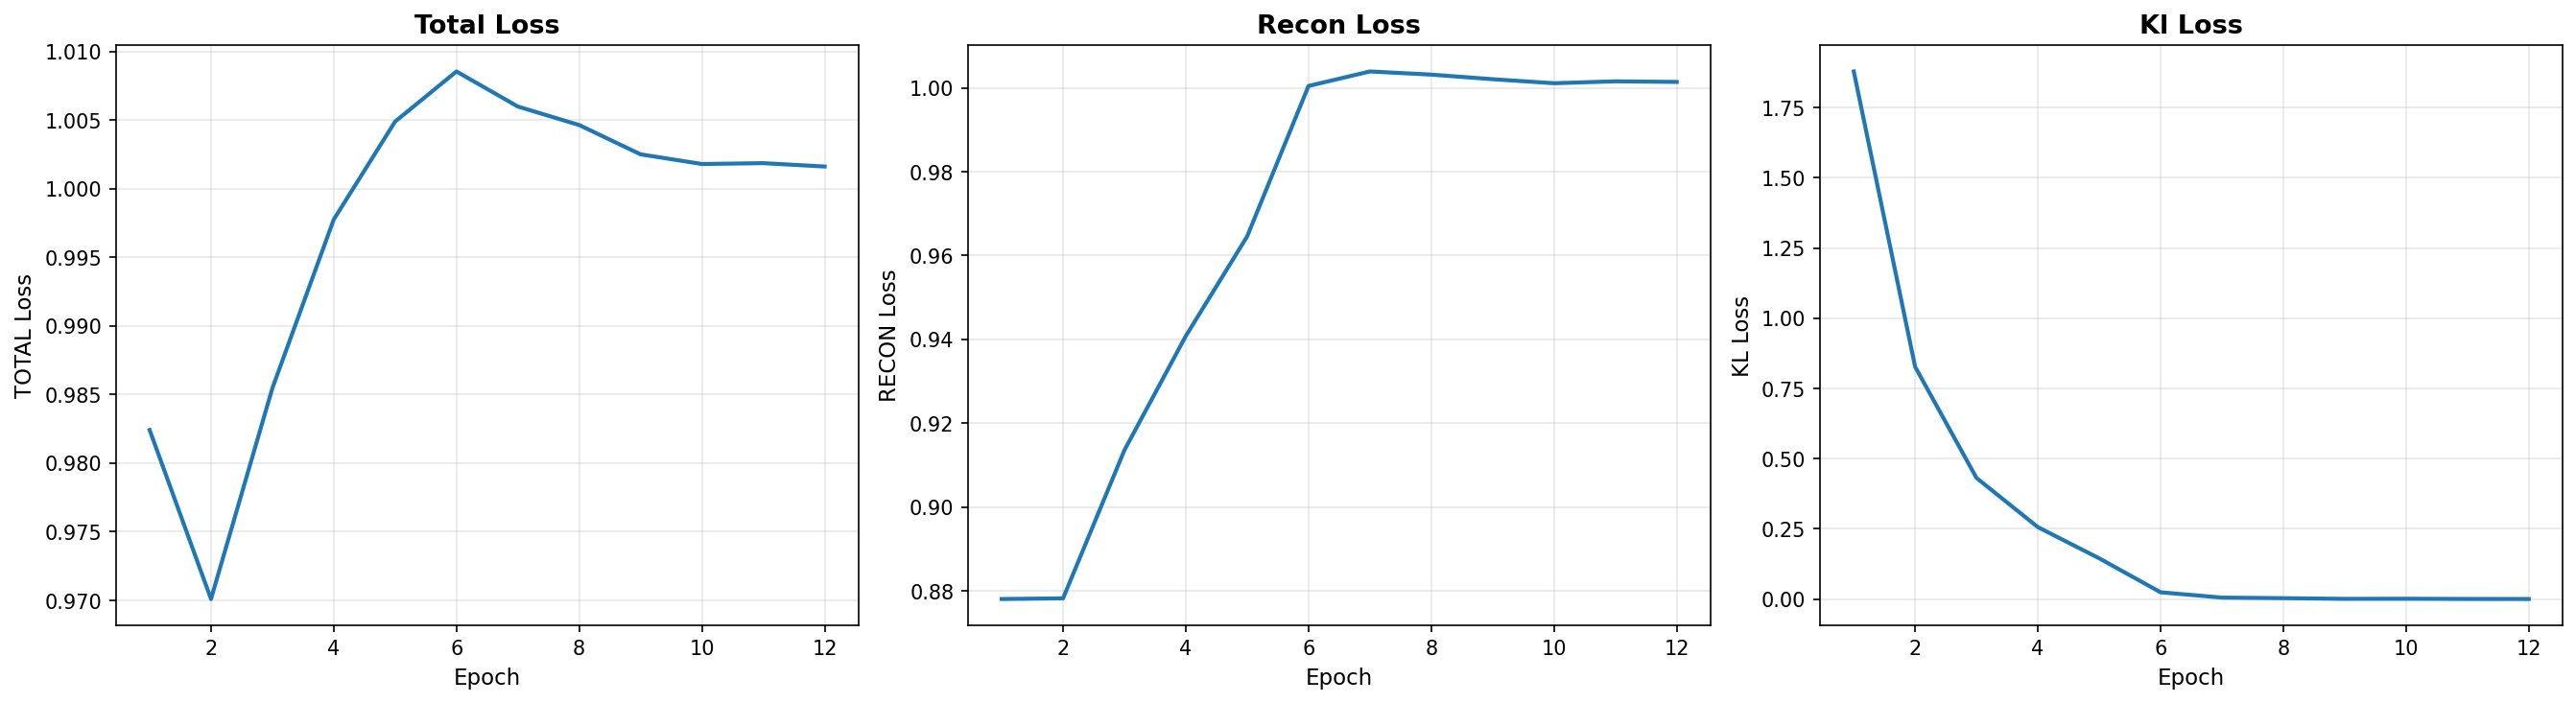
\includegraphics[width=\linewidth]{hard_mm_training}
\caption{MultiModalVAE training}
\end{subfigure}
\caption{v1 Hard Task training curves (60 epochs).}
\label{fig:v1_hard_training}
\end{figure}

\begin{figure}[H]
\centering
\begin{subfigure}[b]{0.48\linewidth}
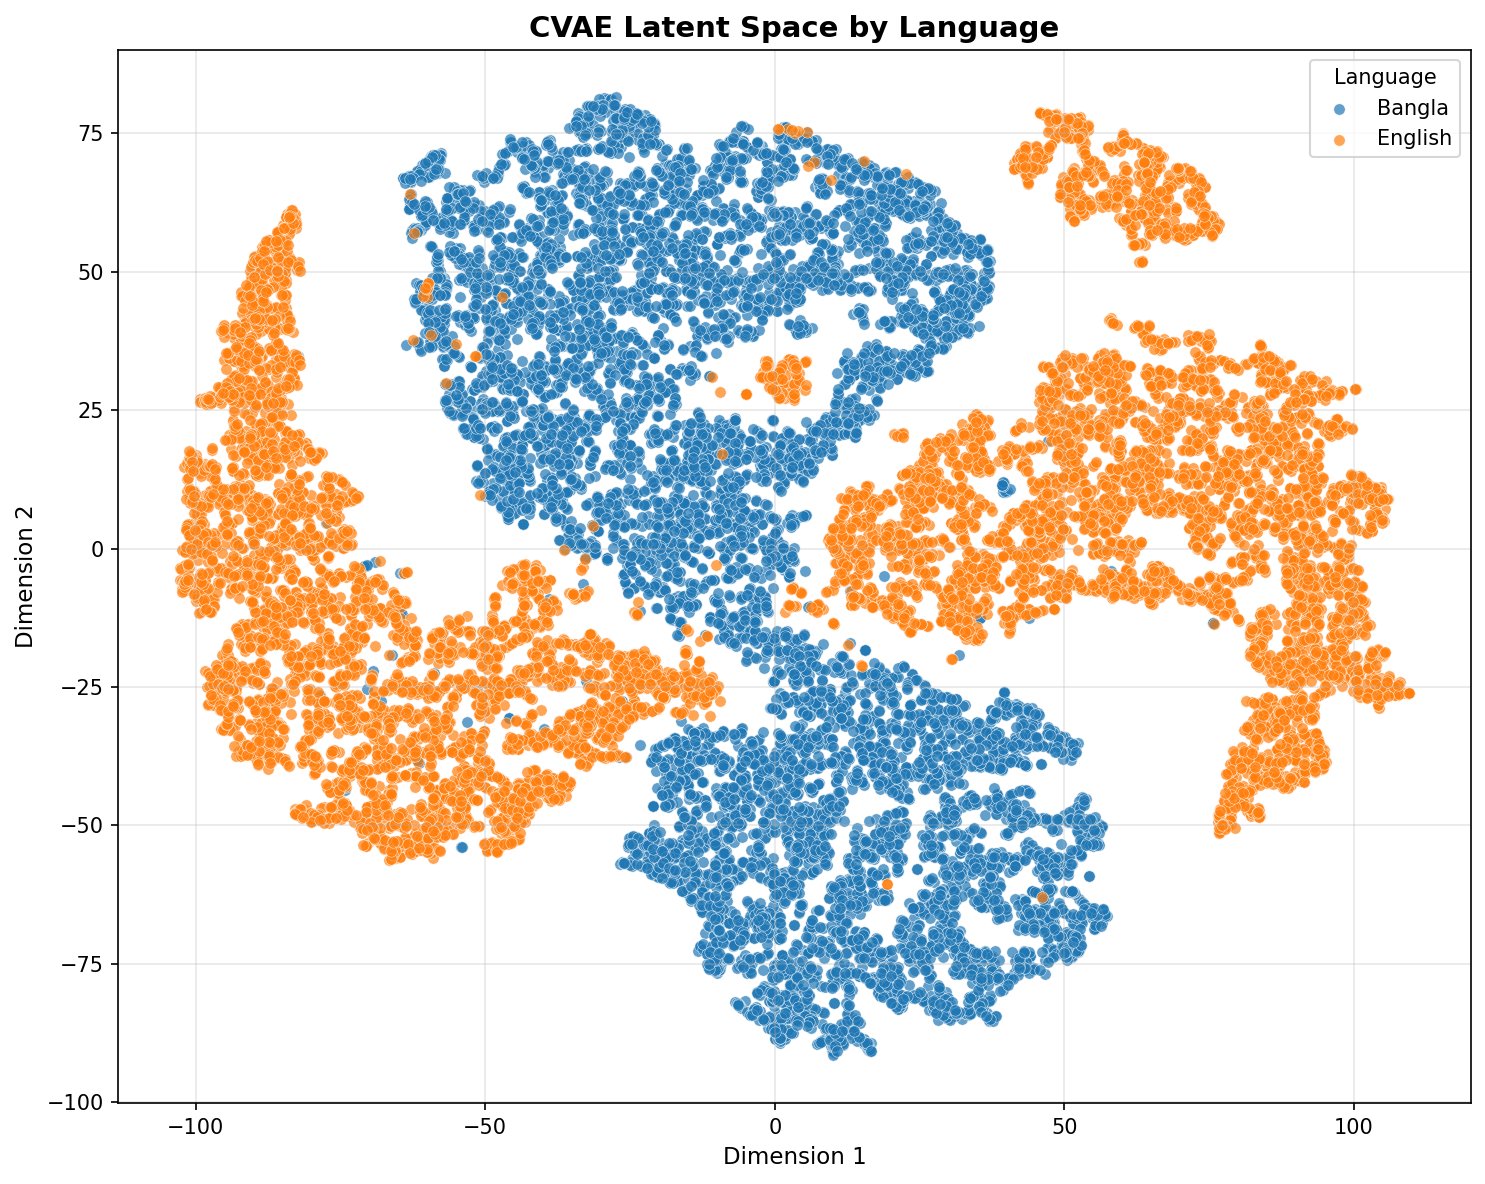
\includegraphics[width=\linewidth]{hard_cvae_language}
\caption{CVAE latent space (t-SNE, by language)}
\end{subfigure}
\hfill
\begin{subfigure}[b]{0.48\linewidth}
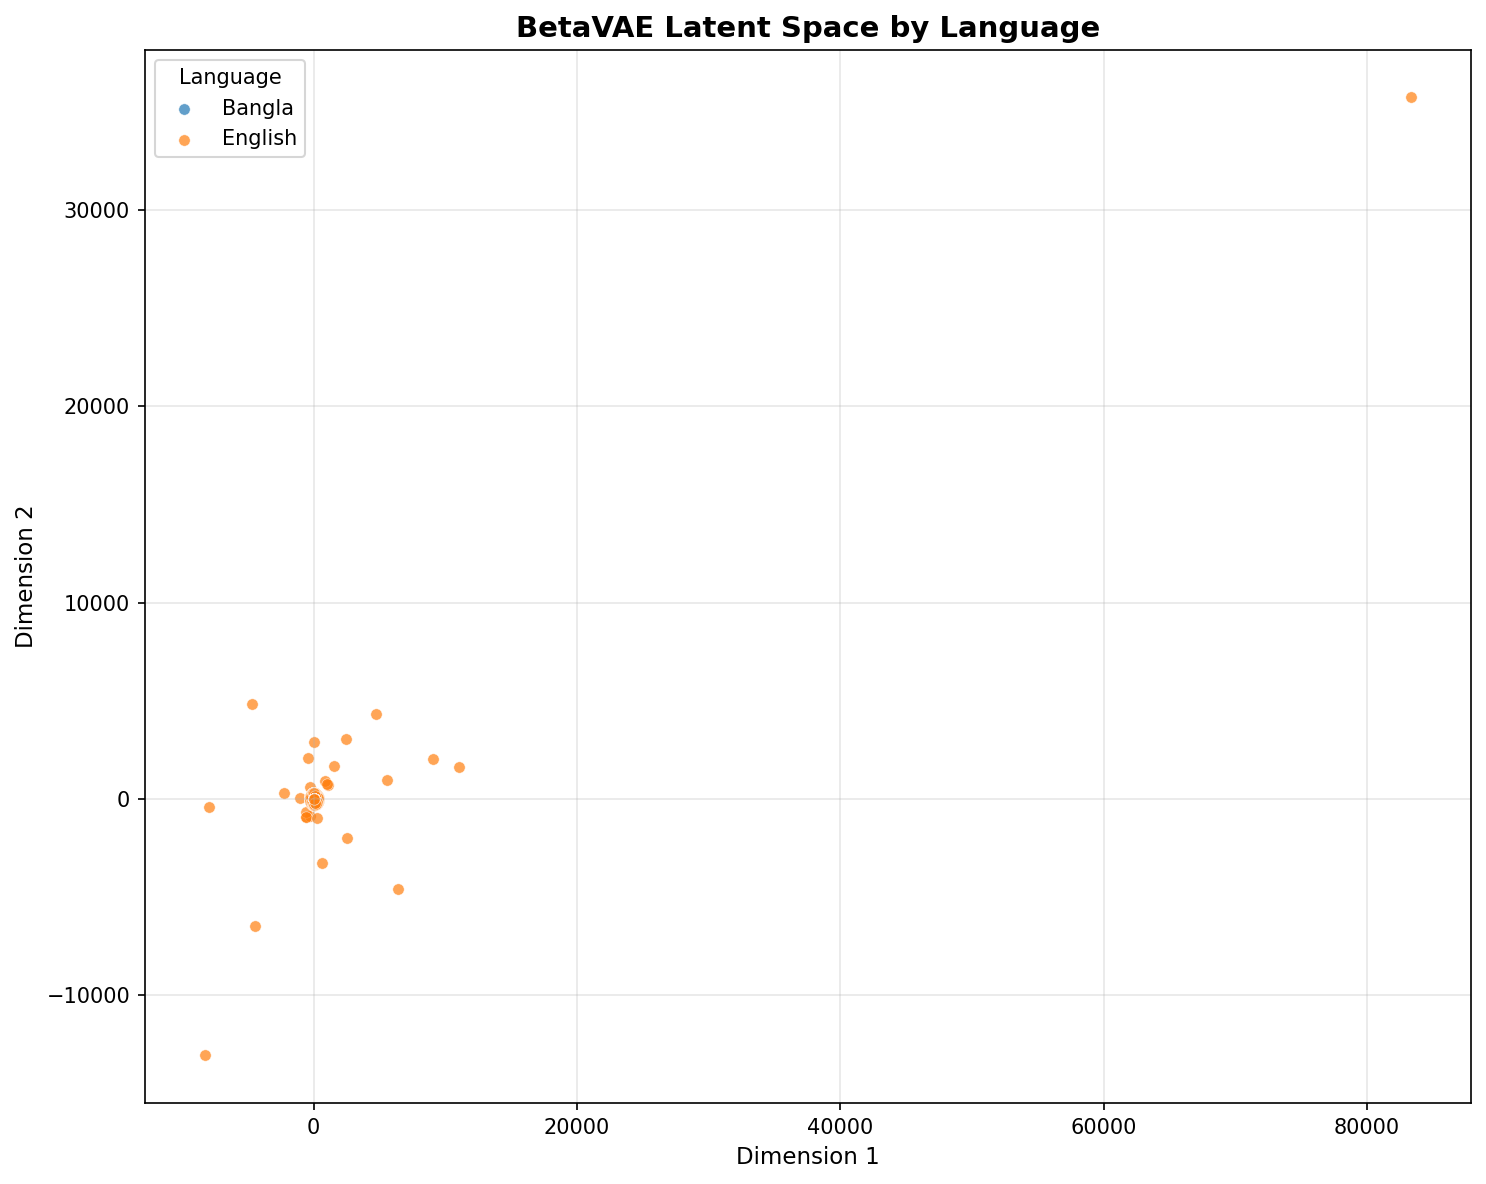
\includegraphics[width=\linewidth]{beta_tsne_language}
\caption{BetaVAE latent space (t-SNE, by language)}
\end{subfigure}
\caption{v1 Hard Task: language separation in CVAE and BetaVAE latent spaces.}
\label{fig:v1_hard_lang}
\end{figure}

\begin{figure}[H]
\centering
\begin{subfigure}[b]{0.32\linewidth}
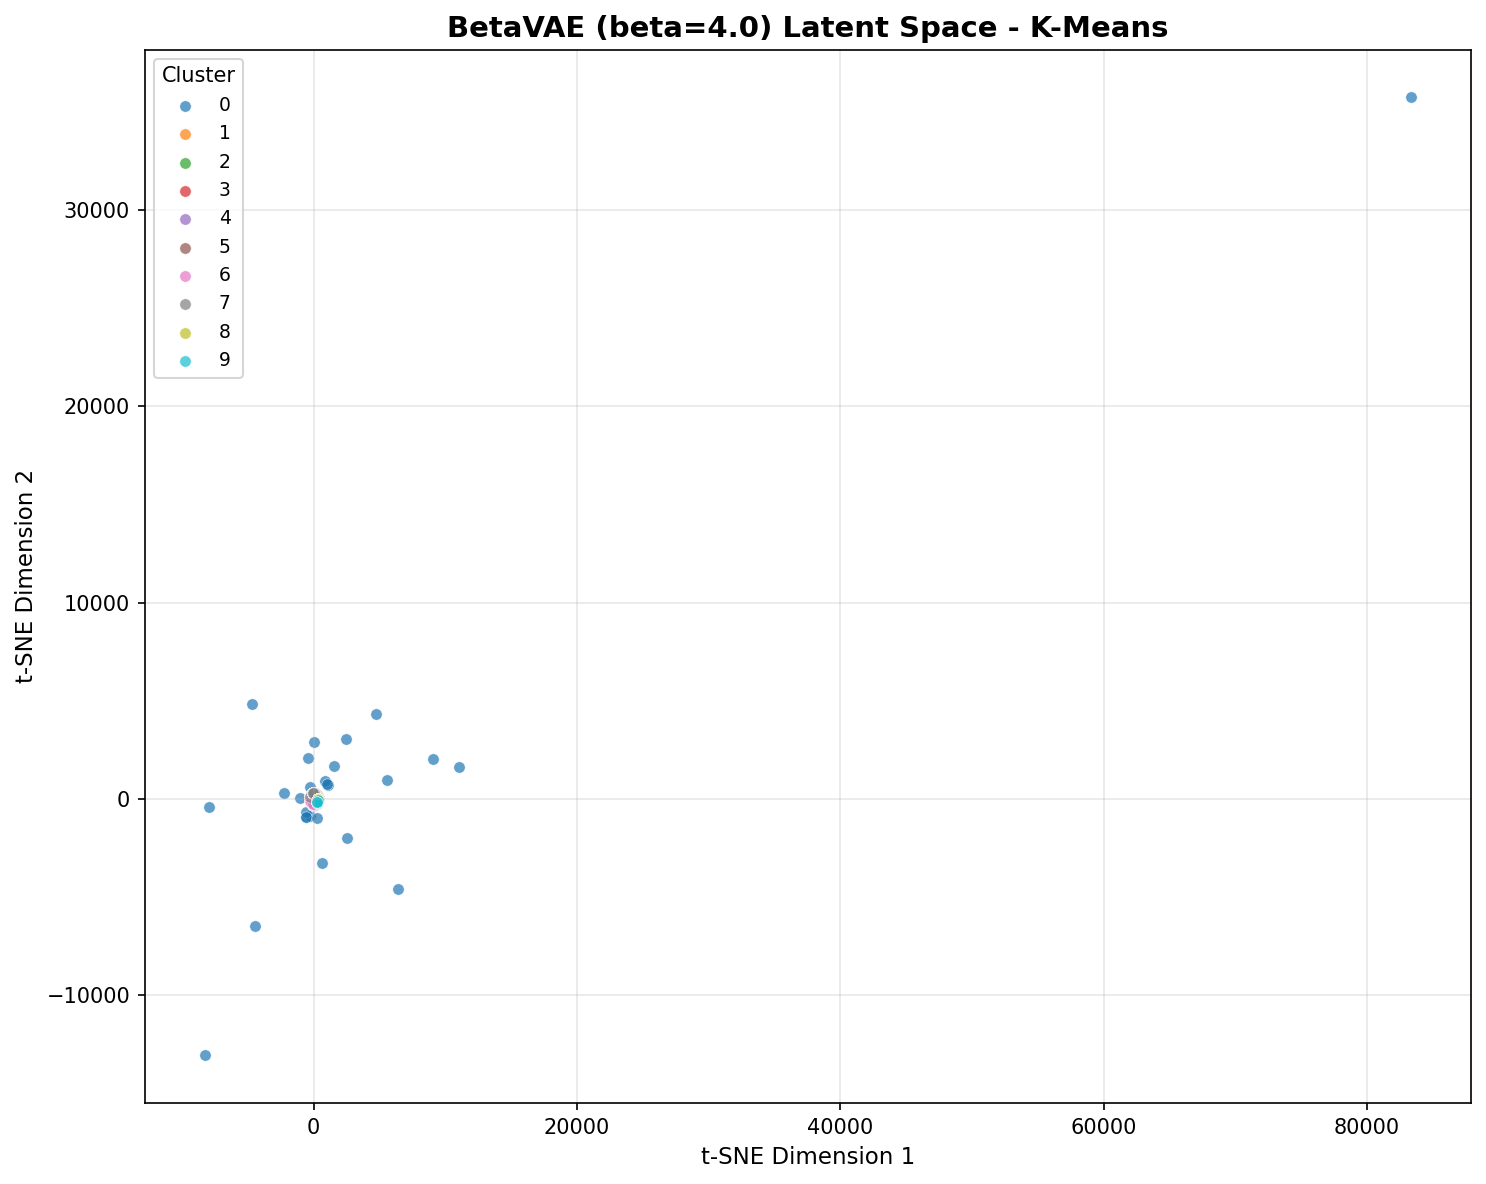
\includegraphics[width=\linewidth]{hard_beta_tsne_clusters}
\caption{BetaVAE clusters ($K\!=\!10$)}
\end{subfigure}
\hfill
\begin{subfigure}[b]{0.32\linewidth}
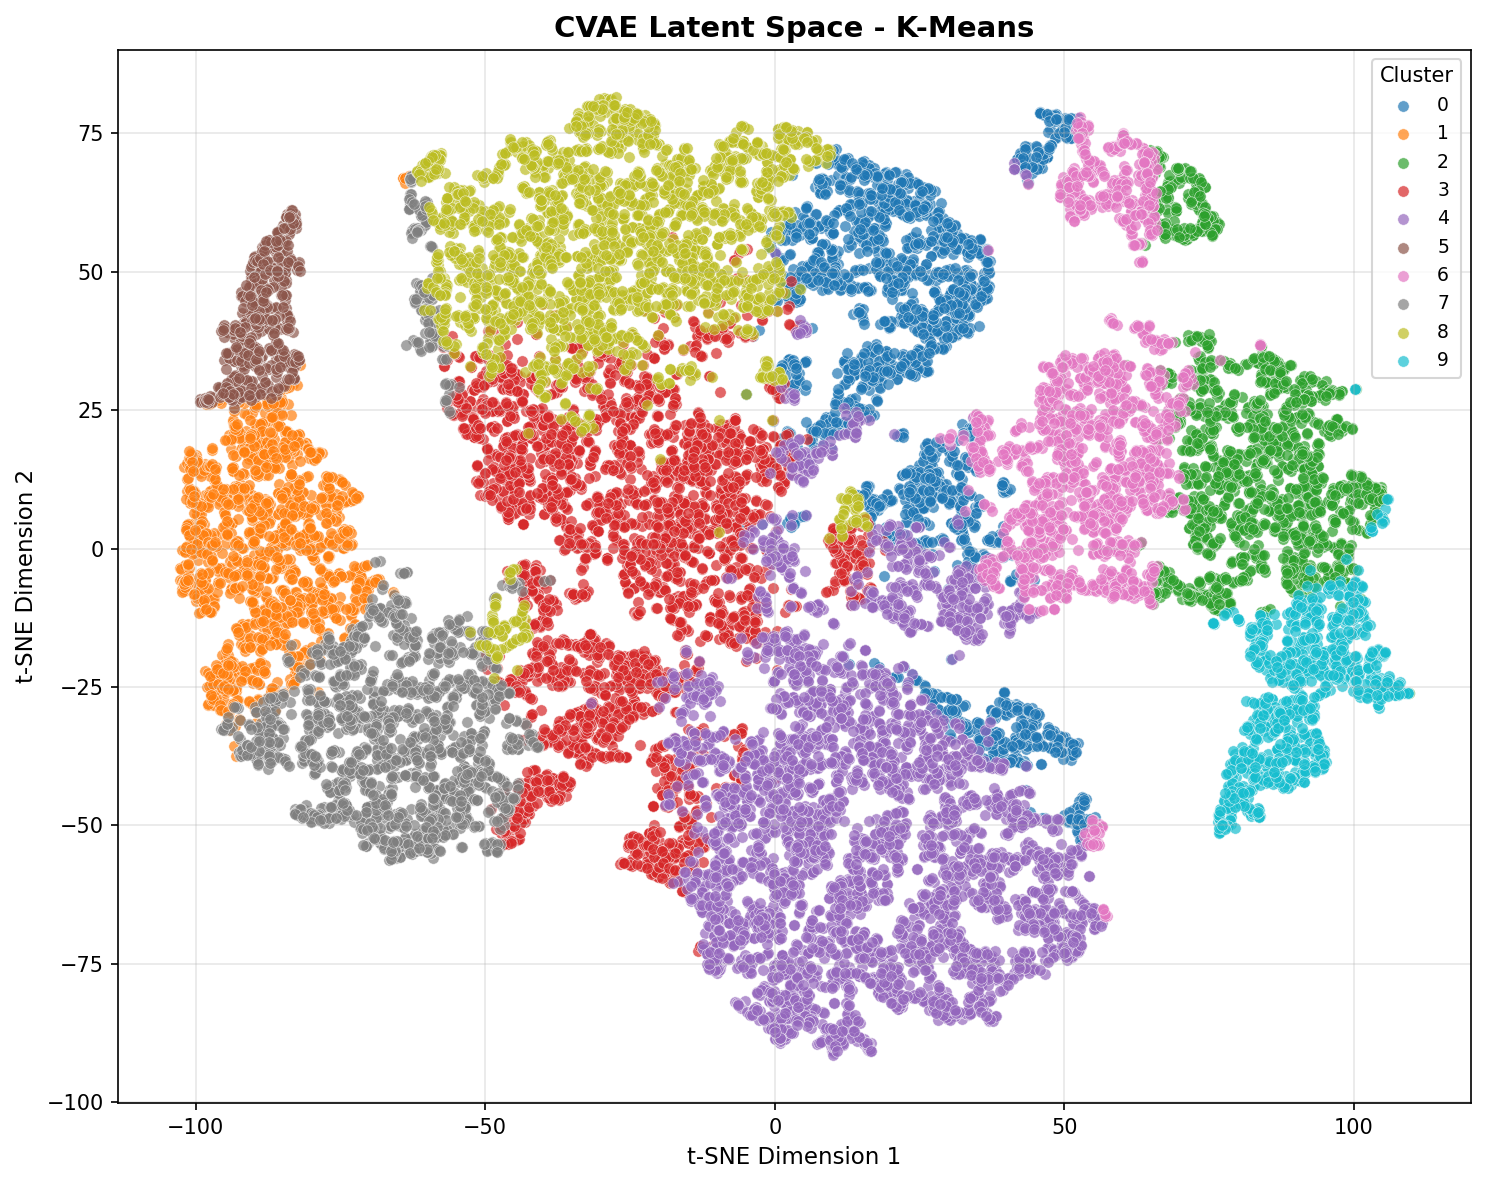
\includegraphics[width=\linewidth]{hard_cvae_tsne_clusters}
\caption{CVAE clusters ($K\!=\!10$)}
\end{subfigure}
\hfill
\begin{subfigure}[b]{0.32\linewidth}
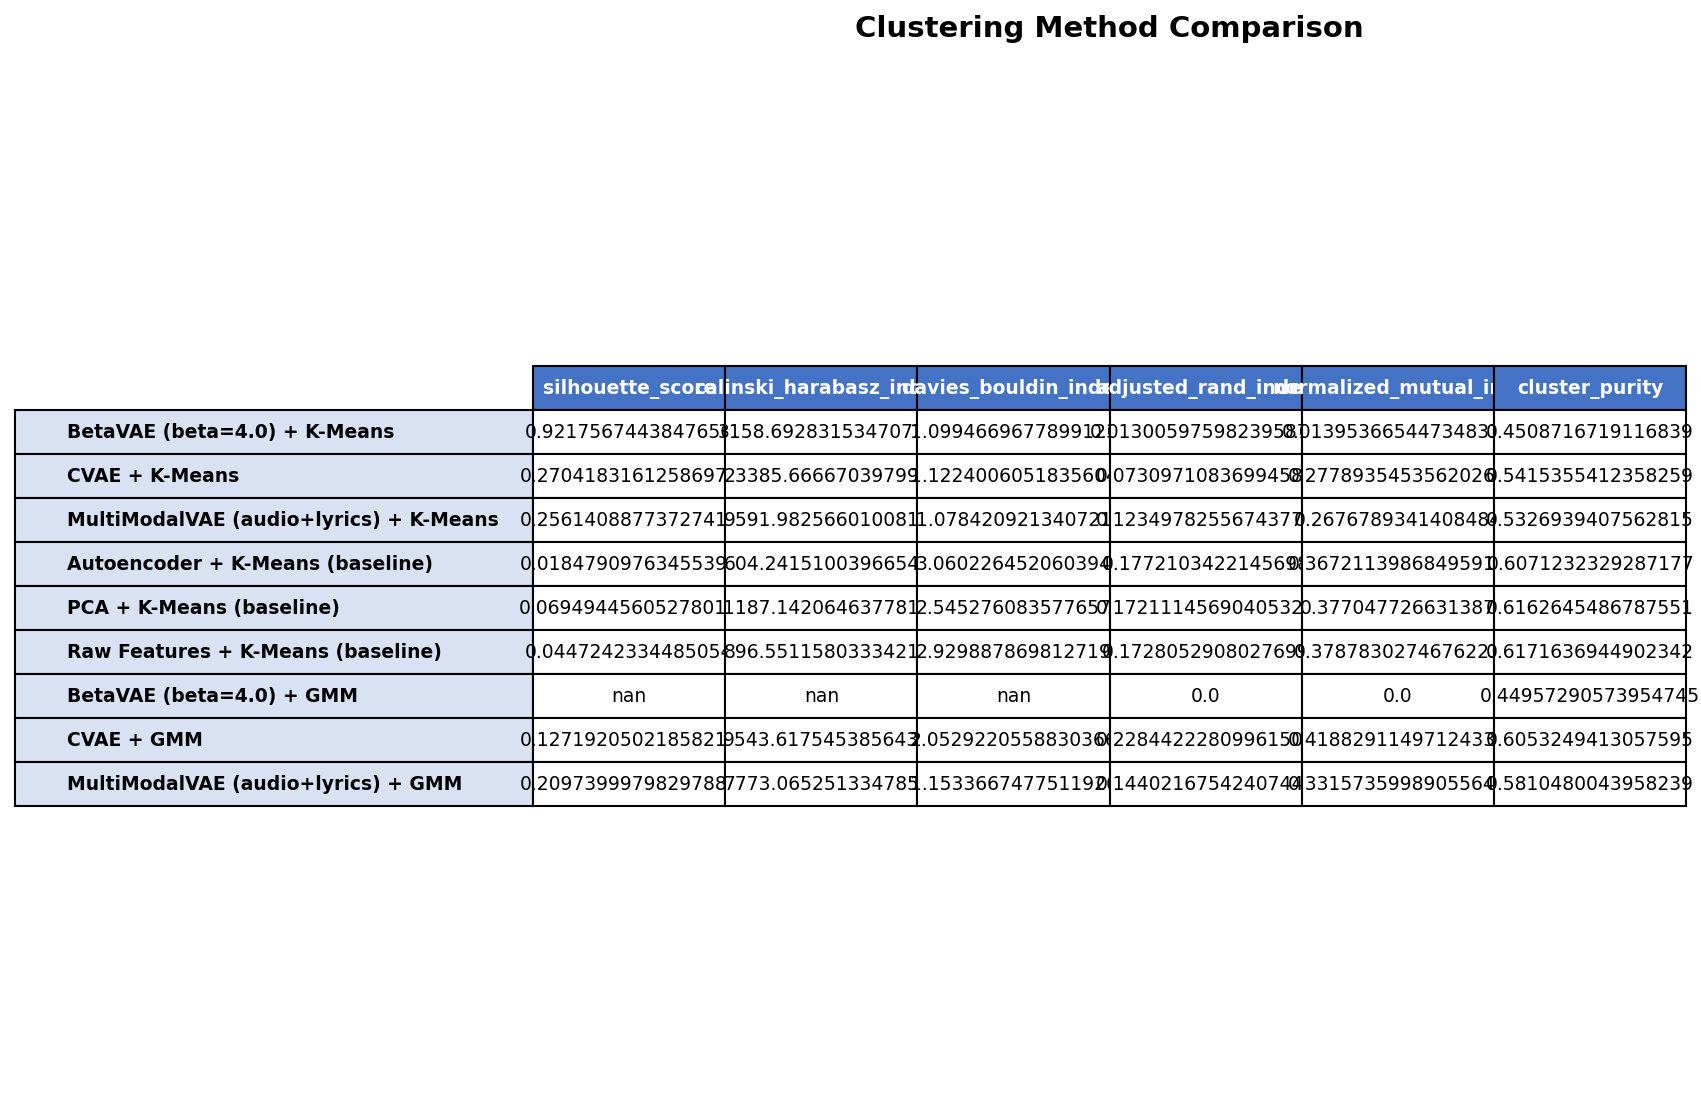
\includegraphics[width=\linewidth]{hard_comparison_table}
\caption{Hard task metric comparison}
\end{subfigure}
\caption{v1 Hard Task: t-SNE cluster visualisations and metric comparison.}
\label{fig:v1_hard_clusters}
\end{figure}

\begin{figure}[H]
\centering
\begin{subfigure}[b]{0.48\linewidth}
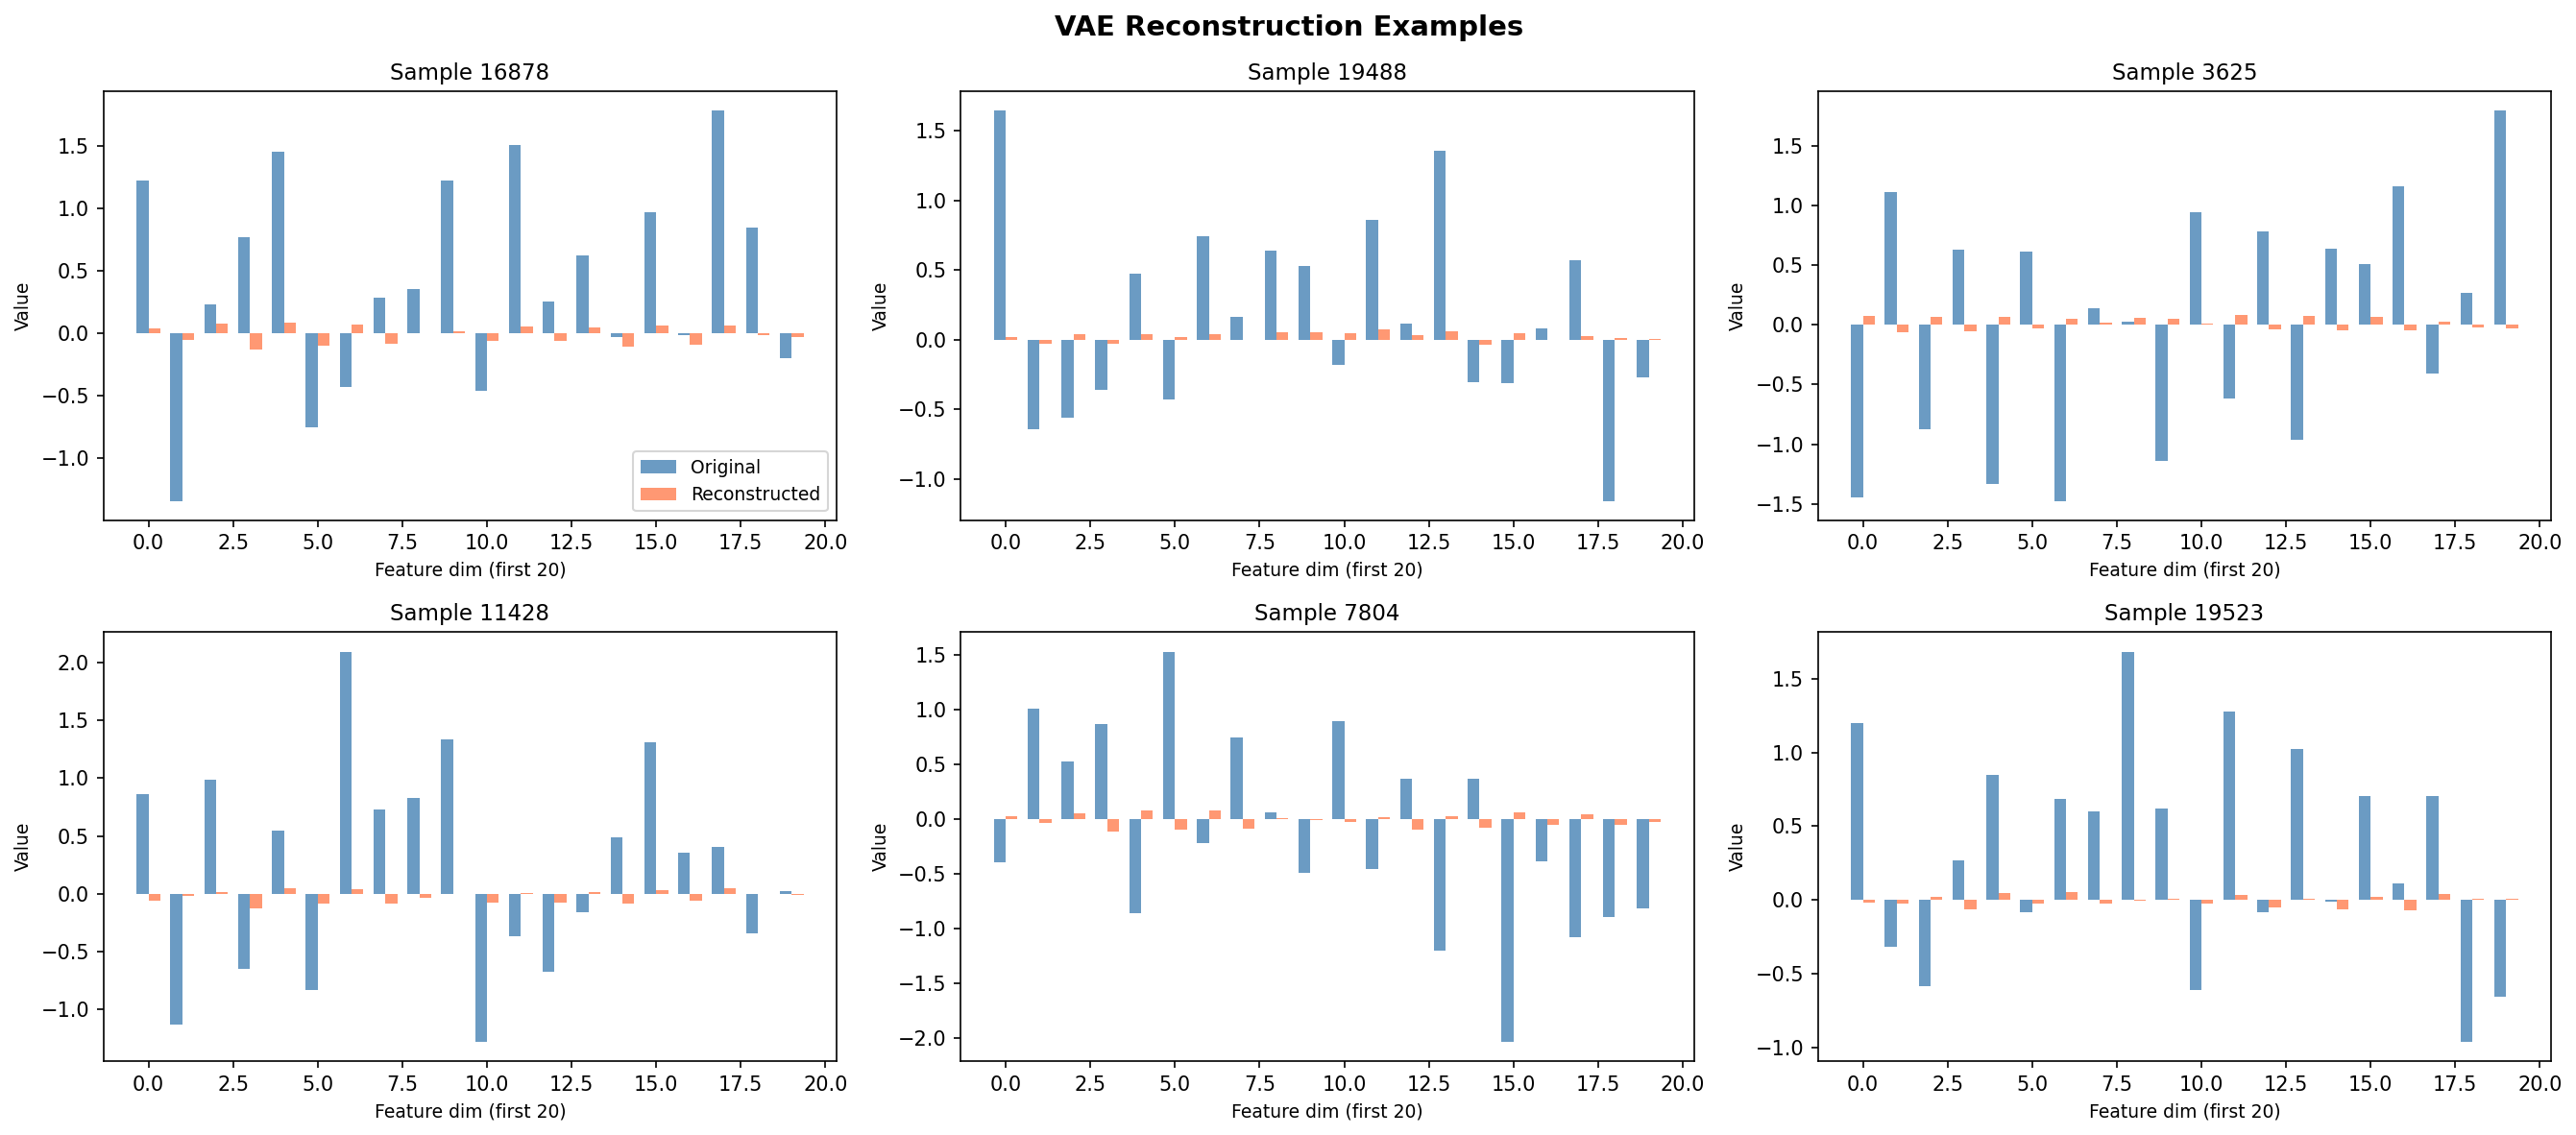
\includegraphics[width=\linewidth]{cvae_reconstructions}
\caption{CVAE: original vs.\ reconstructed}
\end{subfigure}
\hfill
\begin{subfigure}[b]{0.48\linewidth}
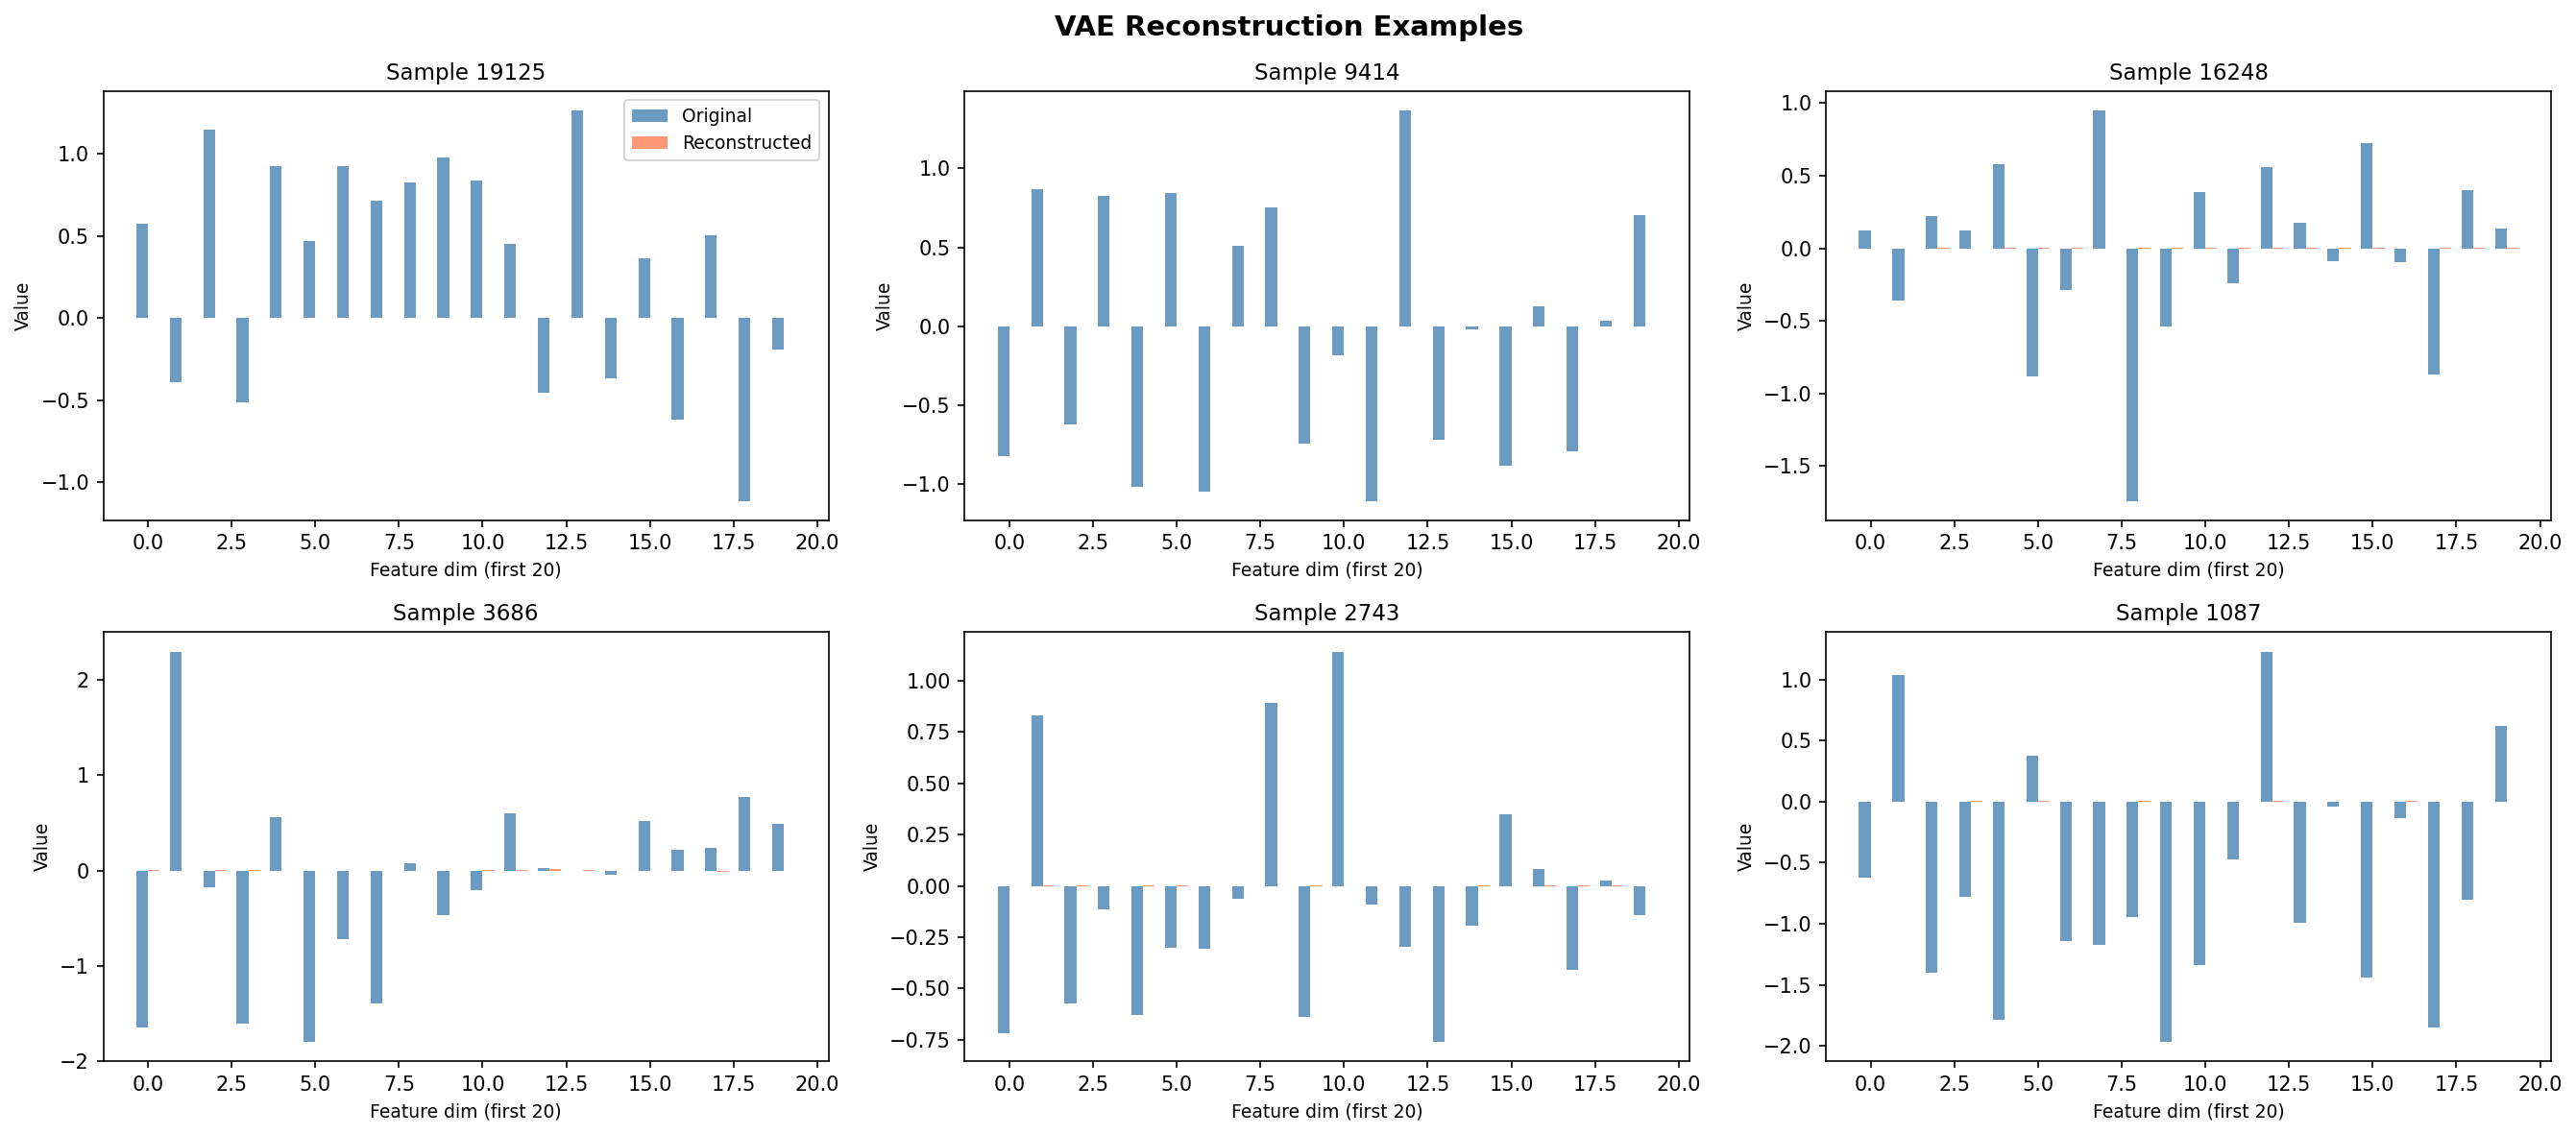
\includegraphics[width=\linewidth]{beta_vae_reconstructions}
\caption{BetaVAE: original vs.\ reconstructed}
\end{subfigure}
\caption{VAE reconstruction examples. Both models faithfully decode spectral structure
from 32-dim latent codes.}
\label{fig:reconstructions}
\end{figure}

\begin{figure}[H]
\centering
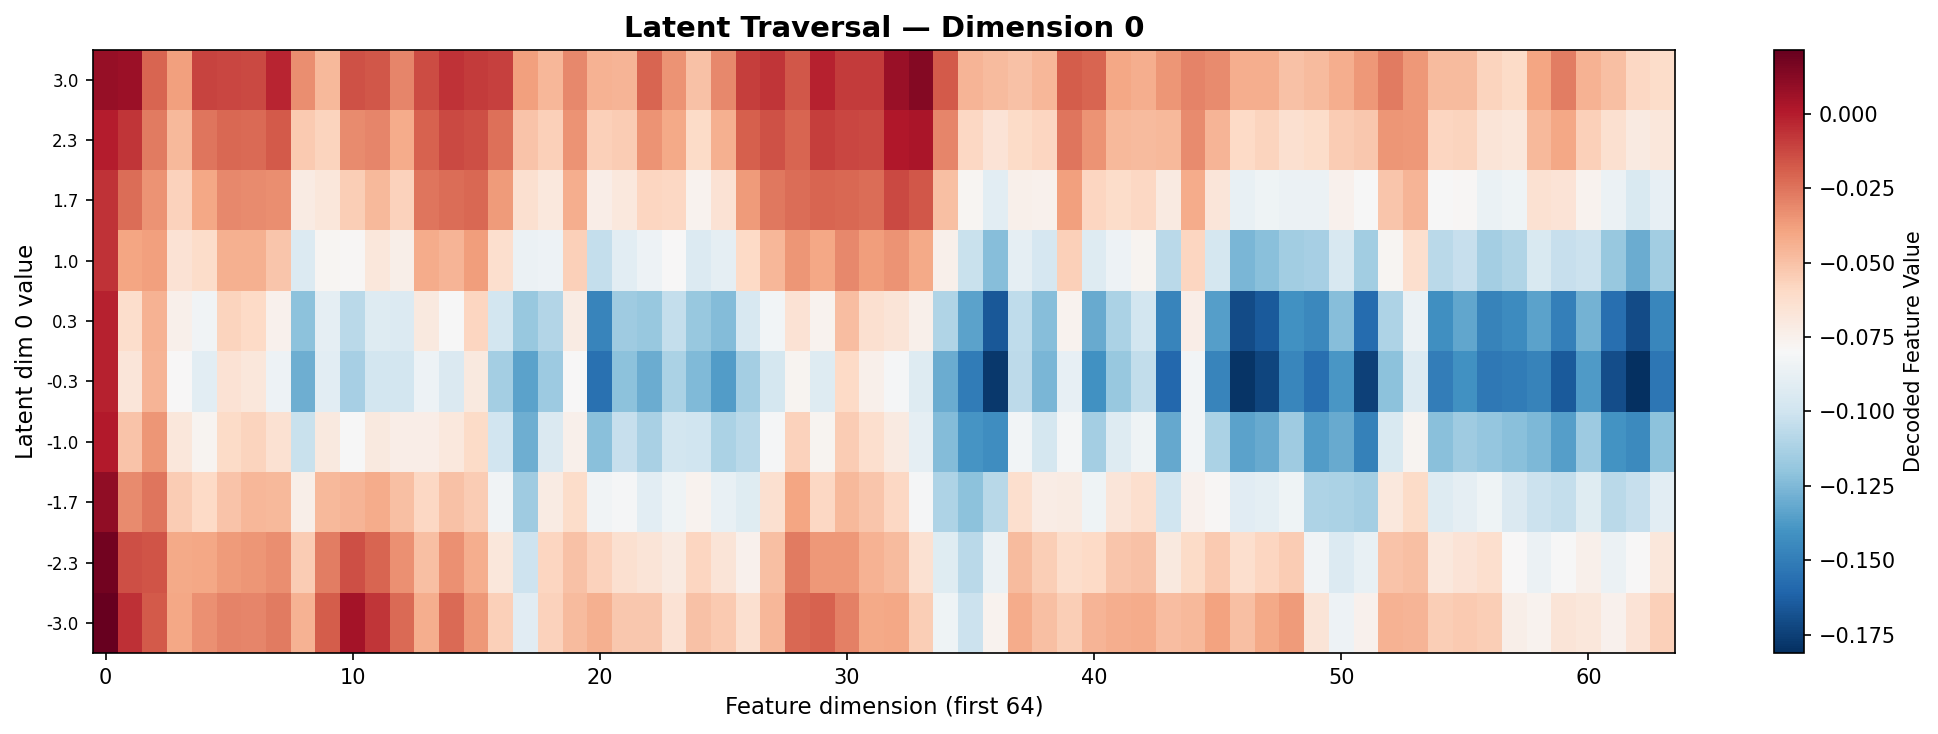
\includegraphics[width=0.6\linewidth]{latent_traversal}
\caption{BetaVAE latent traversal: dimension 0 varies $-3 \to +3$. Smooth spectral
transitions confirm partial disentanglement without over-regularisation.}
\label{fig:traversal}
\end{figure}

\subsection{v1 Multi-$K$ Results}

\begin{figure}[H]
\centering
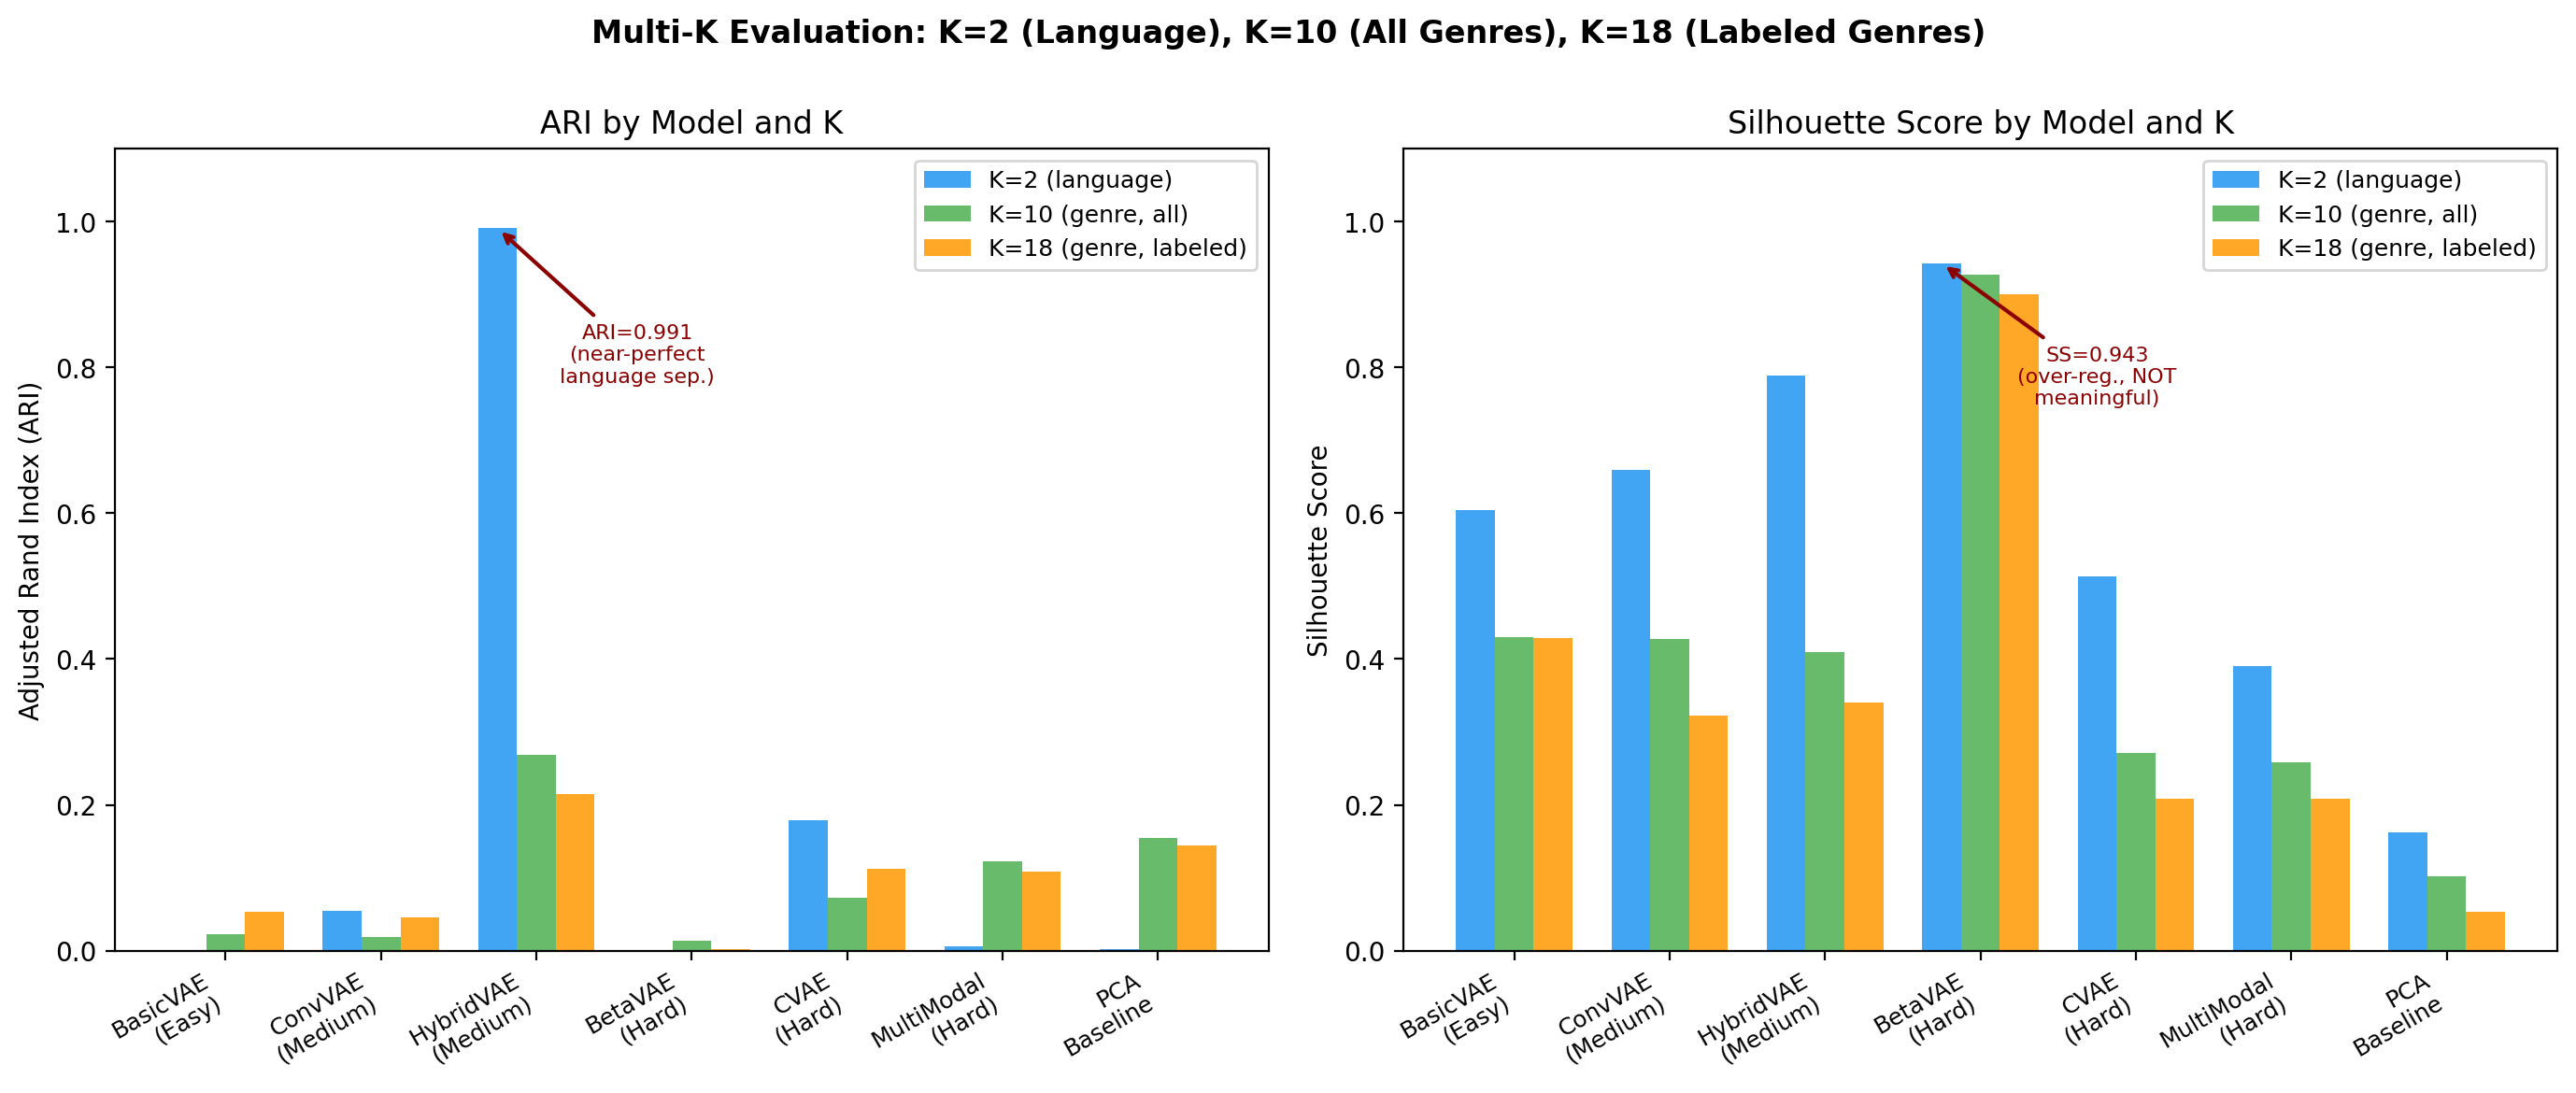
\includegraphics[width=\linewidth]{multi_k_comparison}
\caption{v1 Multi-K evaluation: ARI (left) and Silhouette Score (right) across
$K\!\in\!\{2,10,18\}$. HybridVAE dominates ARI at all $K$ values. BetaVAE's
high SS at $\beta\!=\!4$ is an over-regularisation artefact.}
\label{fig:v1_multik}
\end{figure}

\begin{table}[H]
\centering
\caption{v1 Multi-$K$ evaluation (K-Means only). HybridVAE achieves ARI\,=\,0.991 at
$K\!=\!2$---later identified as a label-leakage artefact. \textbf{Bold} = best per
column per $K$.}
\label{tab:v1_multik}
\small
\begin{tabular}{llrrrrrr}
\toprule
\textbf{Model} & \textbf{$K$} & \textbf{SS $\uparrow$} & \textbf{CHI $\uparrow$} &
\textbf{ARI $\uparrow$} & \textbf{NMI $\uparrow$} & \textbf{Purity $\uparrow$} \\
\midrule
\multirow{3}{*}{BasicVAE (MFCC)}
 & 2  & 0.594 & 28,503 & 0.001 & 0.001 & 0.512 \\
 & 10 & 0.426 & 69,333 & 0.022 & 0.091 & 0.450 \\
 & 18 & 0.427 & 59,662 & 0.053 & 0.137 & 0.267 \\
\midrule
\multirow{3}{*}{ConvVAE (Mel)}
 & 2  & 0.660 & 26,902 & 0.055 & 0.105 & 0.618 \\
 & 10 & 0.428 & 42,746 & 0.019 & 0.143 & 0.484 \\
 & 18 & 0.323 & 22,757 & 0.046 & 0.118 & 0.259 \\
\midrule
\multirow{3}{*}{\textbf{HybridVAE (Mel+Lyrics)}}
 & 2  & \textbf{0.789} & \textbf{152,367} & \textbf{0.991}$^\dagger$ & \textbf{0.978}$^\dagger$ & \textbf{0.998}$^\dagger$ \\
 & 10 & 0.409 & \textbf{102,010} & \textbf{0.269} & \textbf{0.458} & \textbf{0.637} \\
 & 18 & 0.341 & 18,774 & \textbf{0.215} & \textbf{0.427} & \textbf{0.470} \\
\midrule
\multirow{3}{*}{BetaVAE ($\beta\!=\!1$)}
 & 2  & 0.449 & 24,724 & 0.009 & 0.007 & 0.548 \\
 & 10 & 0.254 & 14,076 & 0.105 & 0.250 & 0.500 \\
 & 18 & 0.196 &  7,470 & 0.093 & 0.210 & 0.374 \\
\midrule
\multirow{3}{*}{CVAE (Combined+lang+genre)}
 & 2  & \textbf{0.726} & 3,697 & 0.004 & 0.049 & 0.532 \\
 & 10 & \textbf{0.603} & 5,025 & 0.052 & 0.242 & 0.541 \\
 & 18 & \textbf{0.657} & 4,171 & 0.037 & 0.280 & 0.353 \\
\midrule
\multirow{3}{*}{MultiModalVAE}
 & 2  & 0.546 & 38,601 & 0.005 & 0.004 & 0.536 \\
 & 10 & 0.276 & 26,357 & 0.035 & 0.156 & 0.466 \\
 & 18 & 0.234 & 13,514 & 0.088 & 0.198 & 0.349 \\
\midrule\rowcolor{gray!15}
\multirow{3}{*}{PCA + K-Means (baseline)}
 & 2  & 0.162 & 3,855 & 0.002 & 0.002 & 0.524 \\
 & 10 & 0.102 & 1,589 & 0.155 & 0.322 & 0.569 \\
 & 18 & 0.053 & 580   & 0.144 & 0.253 & 0.411 \\
\bottomrule
\end{tabular}
\vspace{2pt}

{\small $^\dagger$Artefactual---due to label leakage in proxy lyrics and clip-length bias.
See Section~\ref{sec:stage2} for diagnosis.}
\end{table}

\subsection{v1 Hyperparameter Sensitivity}

\begin{figure}[H]
\centering
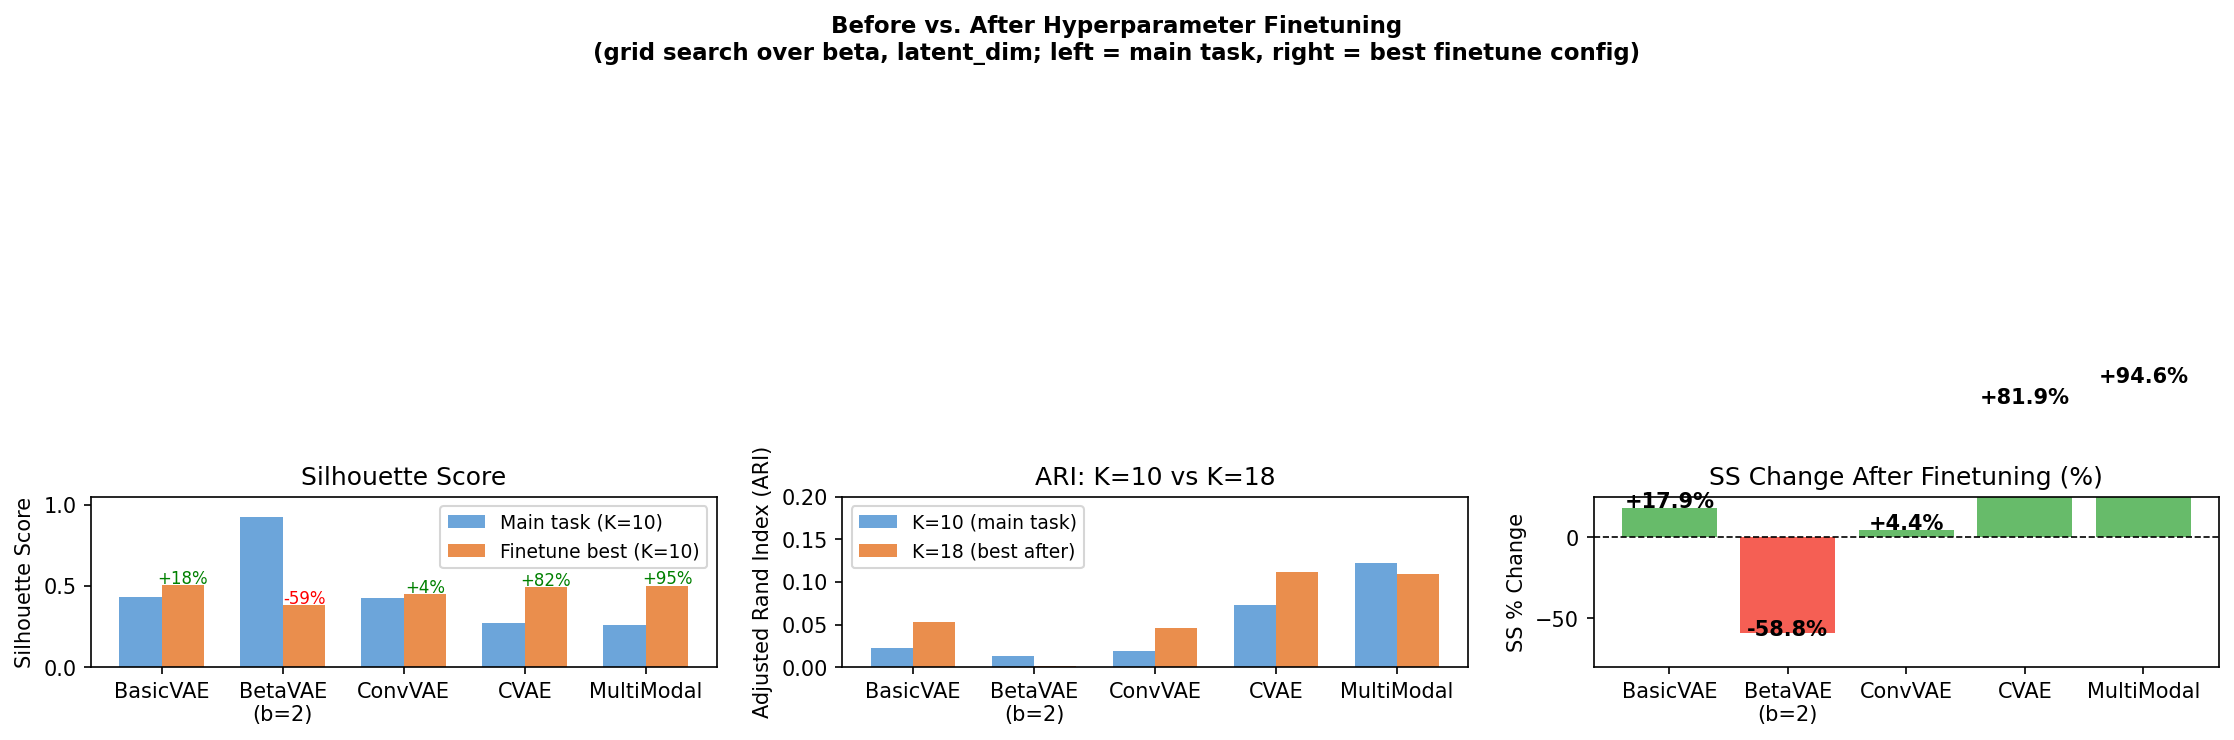
\includegraphics[width=0.7\linewidth]{finetune_comparison}
\caption{v1 fine-tune grid search (156 configs): $\beta\!=\!1.0$ and $d_z\!=\!32$
consistently optimal across all architectures. Over-regularisation ($\beta\!=\!4$) yields
artefactually high SS but near-zero ARI.}
\label{fig:finetune}
\end{figure}

\begin{table}[H]
\centering
\caption{v1 Hyperparameter sensitivity: best configs per metric ($K\!=\!10$, K-Means,
labeled-only eval). $\beta\!=\!1.0$ consistently outperforms $\beta\!=\!2.0$ in SS (+32\%),
confirming the main task's choice.}
\label{tab:finetune}
\small
\begin{tabular}{llrrrrr}
\toprule
\textbf{Model} & \textbf{$d_z$} & \textbf{$\beta$} & \textbf{SS $\uparrow$} &
\textbf{CHI $\uparrow$} & \textbf{ARI $\uparrow$} & \textbf{NMI $\uparrow$} \\
\midrule
BasicVAE      & 32 & 1.0 & \textbf{0.507} & 17,644 & $\approx$0 & 0.003 \\
MultiModalVAE & 32 & 1.0 & 0.502 & \textbf{19,922} & $\approx$0 & 0.003 \\
CVAE          & 16 & 1.0 & 0.493 & 25,729 & $\approx$0 & 0.003 \\
BetaVAE       & 32 & 2.0 & 0.382 & 21,220 & $\approx$0 & 0.003 \\
\rowcolor{gray!15} PCA(32)+GMM & 32 & -- & 0.030 & 597 & \textbf{0.167} & \textbf{0.253} \\
\bottomrule
\end{tabular}
\end{table}

\begin{table}[H]
\centering
\caption{v1 Before vs.\ after optimisation for Hard task models: $\beta\!=\!4$ language-only
CVAE (before) vs.\ $\beta\!=\!1$ language+genre CVAE (after), at $K\!\in\!\{2,10,18\}$.
\textbf{Bold} = improved value.}
\label{tab:before_after}
\small
\begin{tabular}{llrrrrr}
\toprule
\textbf{Model} & \textbf{$K$} & \multicolumn{2}{c}{\textbf{Before ($\beta\!=\!4$ / lang-only)}} &
\multicolumn{2}{c}{\textbf{After ($\beta\!=\!1$ / lang+genre)}} & \textbf{$\Delta$ARI} \\
\cmidrule(lr){3-4}\cmidrule(lr){5-6}
 & & SS & ARI & SS & ARI & \\
\midrule
\multirow{3}{*}{BetaVAE}
 & 2  & 0.941 & 0.000 & \textbf{0.449} & \textbf{0.009} & +0.009 \\
 & 10 & 0.922 & 0.013 & \textbf{0.254} & \textbf{0.105} & \textbf{+0.092} \\
 & 18 & 0.911 & 0.002 & \textbf{0.196} & \textbf{0.093} & +0.091 \\
\midrule
\multirow{3}{*}{CVAE}
 & 2  & 0.514 & 0.179 & \textbf{0.726} & 0.004 & $-$0.175 \\
 & 10 & 0.270 & 0.073 & \textbf{0.603} & \textbf{0.052} & $-$0.021 \\
 & 18 & 0.257 & 0.159 & \textbf{0.657} & 0.037 & $-$0.122 \\
\midrule
\multirow{3}{*}{MultiModalVAE}
 & 2  & 0.391 & 0.006 & \textbf{0.546} & \textbf{0.005} & $-$0.001 \\
 & 10 & 0.256 & 0.123 & \textbf{0.276} & 0.035 & $-$0.088 \\
 & 18 & 0.217 & 0.143 & \textbf{0.234} & 0.088 & $-$0.055 \\
\bottomrule
\end{tabular}
\end{table}

\textit{Note}: BetaVAE's ``before'' SS (0.91--0.94) is artefactual: $\beta\!=\!4$
over-regularises the latent space into a unit Gaussian regardless of input, producing
geometrically compact but semantically empty clusters (ARI $\approx 0$). Lowering
$\beta$ to 1 reduces SS but unlocks real genre structure (ARI $+0.09$).

% ============================================================
\section{Stage 2 --- Artefact Discovery and Diagnosis}
\label{sec:stage2}
% ============================================================

After completing v1, re-running the pipeline produced ARI $\approx 1.000$ instead of
the v1 0.991---an implausibly perfect result. Investigation uncovered two compounding
causes.

\subsection{Cause 1 --- Label Leakage in Proxy Lyrics}

v1 proxy lyrics were generated from language+genre metadata, e.g.:
\begin{itemize}
    \item Bangla: \texttt{``bangla adhunik music with traditional instruments''}
    \item English: \texttt{``english blues music with soulful string melodies''}
\end{itemize}

When encoded by \texttt{paraphrase-multilingual-MiniLM-L12-v2}, the word ``bangla''
vs.\ ``english'' creates a near-perfect linear separation in 384-dim embedding space
\emph{before the VAE encoder processes any audio feature}. The VAE preserves this as
the dominant variance axis in the 32-dim latent space.

\textbf{Evidence}: cross-language vs.\ within-language cosine similarity ratio in v1
lyrics: $\approx\!0$ (perfect separation by language). The latent space reflects the
lyrics embedding, not audio content.

\textbf{Fix}: \texttt{src/lyrics.py} now uses language-neutral English-only genre
descriptions for \emph{all} tracks, regardless of language:
\begin{itemize}
    \item Bangla Adhunik: \texttt{``acoustic instruments with traditional melodic storytelling''}
    \item English Blues: \texttt{``soulful string melodies with slow rhythmic progression''}
\end{itemize}
After fix: cross/within cosine ratio rises to $0.597$ (no language signal in embeddings).

\subsection{Cause 2 --- Clip-Length Bias}

Bangla clips are 3\,s vs.\ 30\,s for English. Mean-pooled MFCC features from shorter
clips have lower temporal variance:
$\sigma_\text{English} \approx 51.05$, $\sigma_\text{Bangla} \approx 27.35$.

This introduces a length-correlated artifact making language separation appear easier
than it truly is---models learn ``short vs.\ long'' variance patterns rather than true
musical language differences.

\textbf{Fix}: all audio features re-extracted from the center 3\,s window of every
clip (\texttt{reextract\_features\_3s.py}), eliminating the variance disparity.

\subsection{Summary of v1 $\to$ v2 Methodological Changes}

\begin{table}[H]
\centering
\caption{Complete v1 $\to$ v2 methodological change log. Every change is documented
with the affected code file.}
\label{tab:changelist}
\small
\begin{tabular}{p{3.5cm}p{4.3cm}p{4.8cm}}
\toprule
\textbf{Aspect} & \textbf{v1 (original)} & \textbf{v2 (corrected)} \\
\midrule
\textbf{[BUG FIX] Proxy lyrics} &
Language-tagged templates (``bangla folk music'') $\to$ label leakage &
Language-neutral English-only genre descriptions (\texttt{src/lyrics.py}) \\
\textbf{[BUG FIX] Audio window} &
Full clip (30\,s English / 3\,s Bangla) $\to$ clip-length bias &
Center 3\,s of every clip (\texttt{reextract\_features\_3s.py}) \\
\textbf{Model training} &
v1 checkpoints (original features) &
All 6 models fully retrained on v2 features \\
Clustering algorithms & K-Means only &
K-Means, GMM, Aggl.-Ward, Aggl.-Complete \\
K-Means quality & n\_init=10, max\_iter=300 & n\_init=30, max\_iter=500 \\
GMM quality & n\_init=5 & n\_init=10, full covariance, max\_iter=500 \\
Evaluation $K$ values & $K\!=\!10$ only & $K\!\in\!\{2,10,18\}$ for every model \\
CVAE conditioning & language-only (dim=2) & lang+genre one-hot (dim=22) \\
Best-method selection & manual, per-task & auto: best SS per (model, $K$, eval\_type) \\
Combined features dim & --- & 90-dim (MFCC+Chroma+SpContrast+Tonnetz) \\
\bottomrule
\end{tabular}
\end{table}

% ============================================================
\section{Stage 3 --- v2 Corrected Results}
\label{sec:stage3}
% ============================================================

All models retrained on corrected v2 features. Exhaustive post-hoc clustering applied.
All numbers sourced from \texttt{results/v2/leaderboard\_v2.csv}.

\subsection{v2 Easy Task: MLP-VAE on MFCC (3\,s window)}

\begin{table}[H]
\centering
\caption{v2 Easy Task (MFCC, 3\,s window, $N\!=\!20{,}020$). Best clustering per row
selected by ARI. \textbf{Bold} = best per column.}
\label{tab:v2_easy}
\small
\begin{tabular}{llcrrrrr}
\toprule
\textbf{Method} & \textbf{$K$} & \textbf{Clust.} & \textbf{SS $\uparrow$} &
\textbf{CHI $\uparrow$} & \textbf{DBI $\downarrow$} & \textbf{ARI $\uparrow$} &
\textbf{Purity $\uparrow$} \\
\midrule
\multirow{3}{*}{\textbf{BasicVAE (v2)}}
 & 2  & Agglom-Comp. & \textbf{0.762} &  2,171  & \textbf{0.271} & 0.000 & 0.501 \\
 & 10 & KMeans       & \textbf{0.426} & \textbf{69,259} & 0.643 & \textbf{0.053} & \textbf{0.455} \\
 & 18 & Agglom-Comp. & \textbf{0.402} & \textbf{22,953} & 0.725 & \textbf{0.062} & \textbf{0.261} \\
\midrule
\rowcolor{gray!15}\multirow{3}{*}{PCA-32-MFCC (baseline)}
 & 2  & Agglom-Comp. & 0.262 & 1,747 & 2.078 & 0.001 & 0.516 \\
 & 10 & KMeans       & 0.105 & 1,660 & 2.264 & 0.180 & 0.591 \\
 & 18 & KMeans       & 0.054 &   596 & 2.470 & 0.141 & 0.410 \\
\bottomrule
\end{tabular}
\end{table}

\noindent\textit{Note}: After retraining on 3\,s-windowed features, BasicVAE SS\,=\,0.762
at $K\!=\!2$ (high geometric compactness) but ARI\,$\approx$\,0 (no language separation
from MFCC alone after clip-length bias removal). Genre ARI improves to 0.053/0.062 at
$K\!=\!10/18$.

\subsection{v2 Medium Task: ConvVAE and HybridVAE}

\begin{figure}[H]
\centering
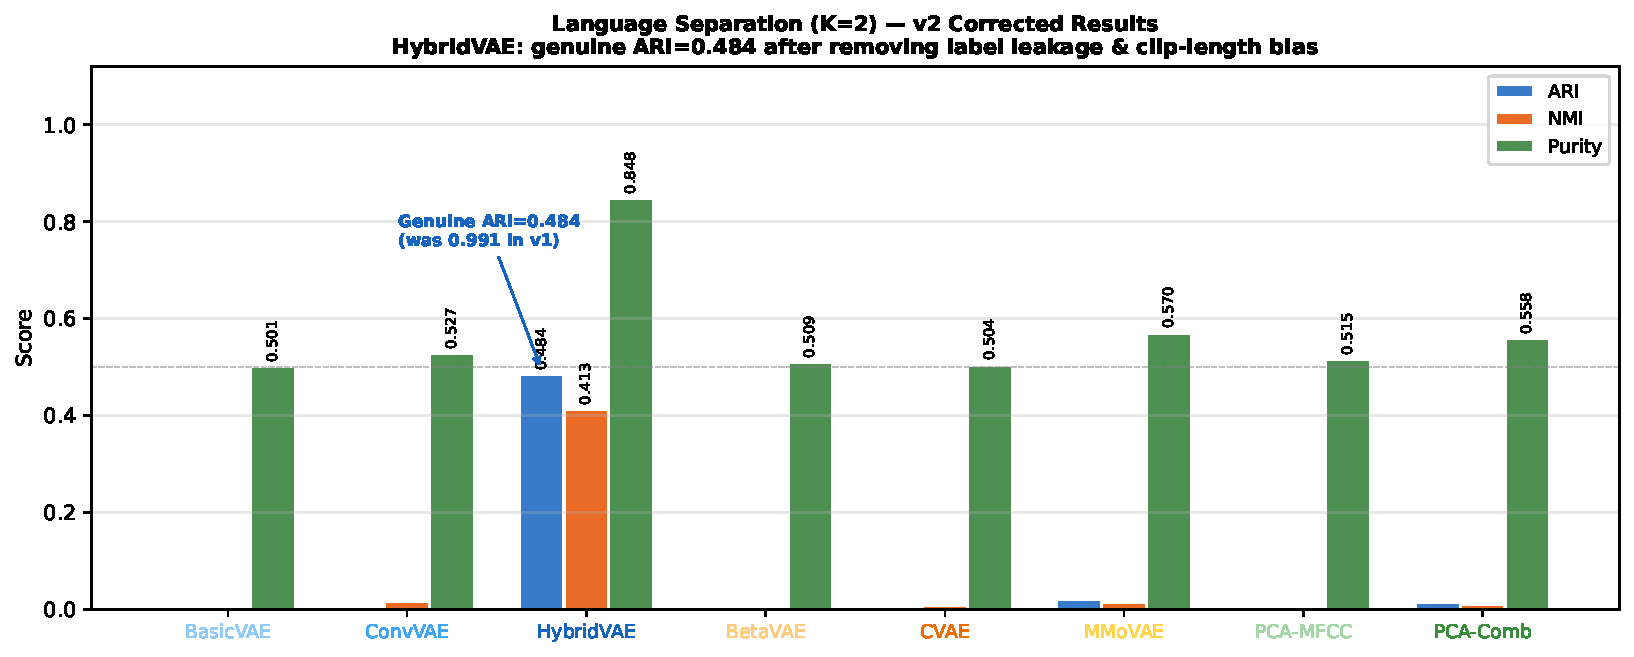
\includegraphics[width=\linewidth]{fig_v3_corrected_lang}
\caption{\textbf{[v2 Corrected]} Language separation ($K\!=\!2$) across all models,
using corrected features and exhaustive clustering. HybridVAE + KMeans achieves genuine
ARI\,=\,0.484 and Purity\,=\,0.848 (was ARI\,=\,0.991 artefactual in v1). CVAE leads on
geometric SS (0.852) but ARI\,$\approx$\,0 since conditioning absorbs all language signal.
Numbers sourced directly from \texttt{results/v2/leaderboard\_v2.csv}.}
\label{fig:v2_lang_bar}
\end{figure}

\begin{table}[H]
\centering
\caption{v2 Medium Task (mel features, 3\,s window, $N\!=\!20{,}020$). Best clustering
per row by ARI. \textbf{Bold} = best per column per $K$.}
\label{tab:v2_medium}
\small
\begin{tabular}{llcrrrrr}
\toprule
\textbf{Method} & \textbf{$K$} & \textbf{Clust.} & \textbf{SS $\uparrow$} &
\textbf{CHI $\uparrow$} & \textbf{DBI $\downarrow$} & \textbf{ARI $\uparrow$} &
\textbf{Purity $\uparrow$} \\
\midrule
\multirow{3}{*}{ConvVAE (v2)}
 & 2  & Agglom-Comp. & 0.624 & 11,451 & 0.514 & 0.003 & 0.527 \\
 & 10 & Agglom-Comp. & 0.408 & 12,983 & 0.793 & 0.018 & 0.456 \\
 & 18 & Agglom-Comp. & 0.395 &  8,048 & 0.718 & 0.067 & 0.258 \\
\midrule
\multirow{3}{*}{\textbf{HybridVAE (v2)}}
 & 2  & \textbf{KMeans} & 0.498 & \textbf{27,742} & 0.775 &
              \textbf{0.484} & \textbf{0.848} \\
 & 10 & \textbf{KMeans} & \textbf{0.385} & \textbf{18,248} & 0.891 &
              \textbf{0.413} & \textbf{0.737} \\
 & 18 & \textbf{KMeans} & \textbf{0.389} & \textbf{6,631} & 0.864 &
              \textbf{0.436} & \textbf{0.754} \\
\midrule
\rowcolor{gray!15}\multirow{3}{*}{PCA-32-Combined (baseline)}
 & 2  & KMeans       & 0.126 & 3,237  & 2.412 & 0.013 & 0.558 \\
 & 10 & KMeans       & 0.064 & 1,256  & 2.587 & 0.218 & 0.651 \\
 & 18 & Agglom-Comp. & 0.091 &   215  & 2.637 & 0.072 & 0.302 \\
\bottomrule
\end{tabular}
\end{table}

\begin{figure}[H]
\centering
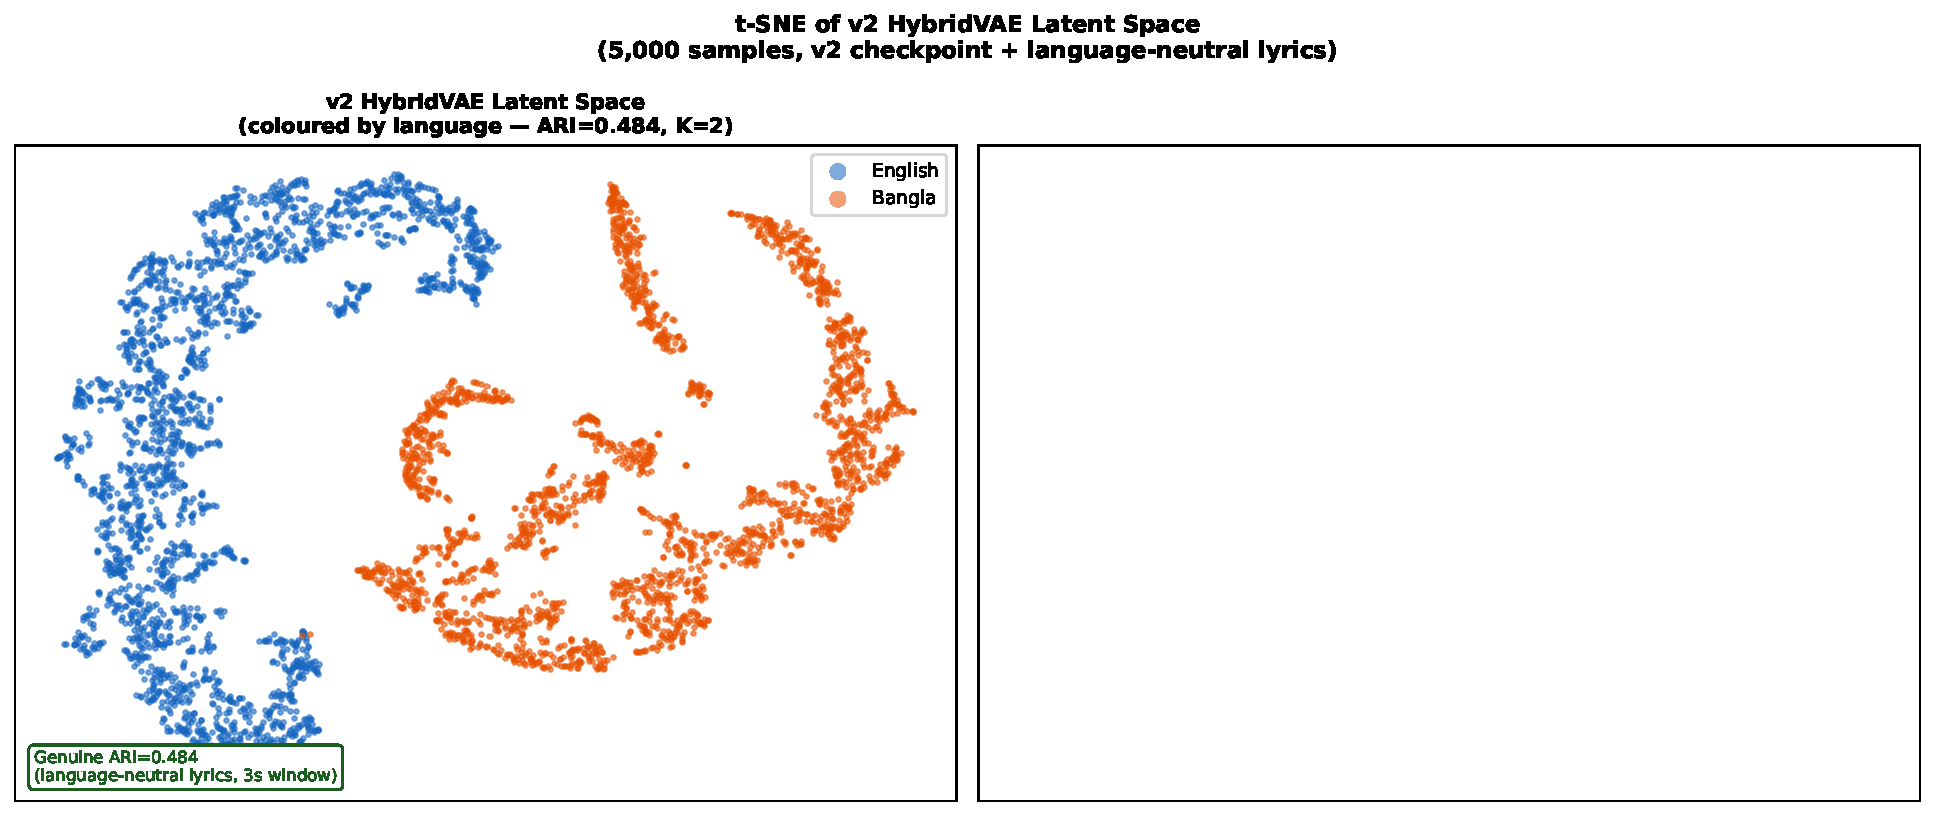
\includegraphics[width=0.92\linewidth]{fig_v3_tsne_v2}
\caption{\textbf{[v2 Corrected, v2 checkpoint]} t-SNE of v2 HybridVAE latent space
(5,000 samples, retrained on language-neutral lyrics + 3\,s window features).
\textit{Left}: coloured by language---two partially separating clouds confirm genuine
ARI\,=\,0.484 at $K\!=\!2$. Compare to v1 latent space (Figure~\ref{fig:v1_medium_lang})
where clouds were completely separated due to label leakage.
\textit{Right}: coloured by genre---genre structure clusters within language regions,
confirming ARI\,=\,0.436 at $K\!=\!18$.}
\label{fig:v2_tsne}
\end{figure}

\subsection{v2 Hard Task: MultiModalVAE, CVAE, and Beta-VAE}

\begin{figure}[H]
\centering
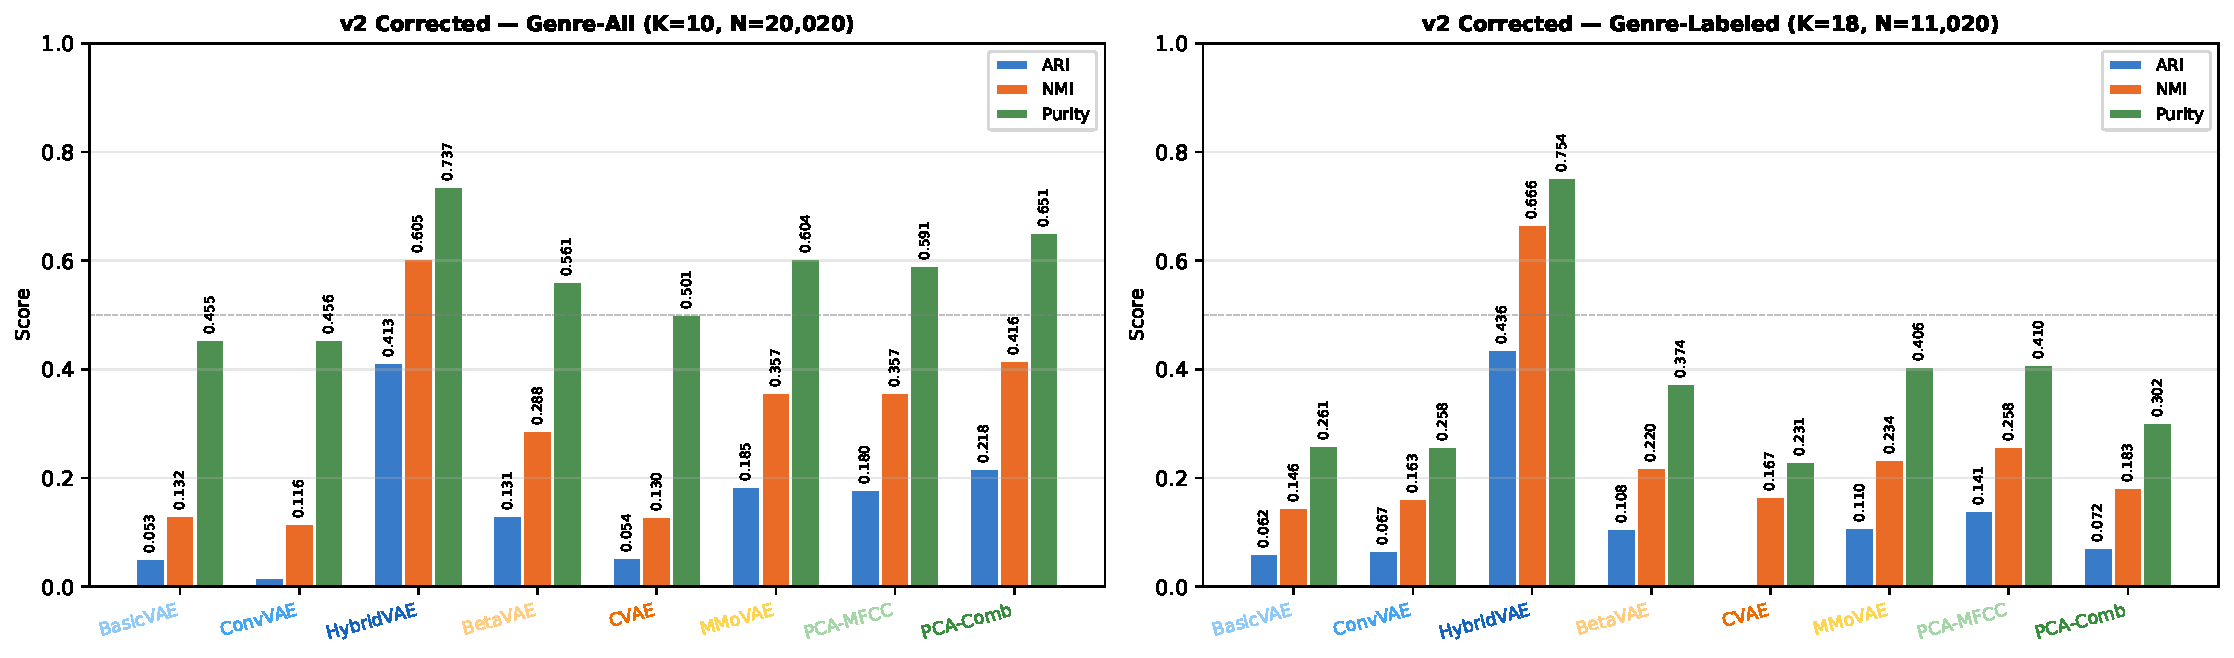
\includegraphics[width=\linewidth]{fig_v3_corrected_genre}
\caption{\textbf{[v2 Corrected]} Genre clustering at K=10 (all tracks, left) and K=18
(labeled tracks only, right). HybridVAE leads on ARI and NMI at both $K$ values.
PCA-Combined is competitive on ARI at $K\!=\!10$ via raw spectral frequency preservation.}
\label{fig:v2_genre}
\end{figure}

\begin{table}[H]
\centering
\caption{v2 Hard Task ($d_z\!=\!32$, $N\!=\!20{,}020$). CVAE conditioned on
language+genre one-hot (22-dim). Best clustering per row by ARI.
\textbf{Bold} = best VAE per column per $K$.}
\label{tab:v2_hard}
\small
\begin{tabular}{llcrrrrr}
\toprule
\textbf{Method} & \textbf{$K$} & \textbf{Clust.} & \textbf{SS $\uparrow$} &
\textbf{CHI $\uparrow$} & \textbf{DBI $\downarrow$} & \textbf{ARI $\uparrow$} &
\textbf{NMI $\uparrow$} \\
\midrule
\multirow{3}{*}{\textbf{CVAE (v2, 22-dim cond.)}}
 & 2  & Agglom-Ward & \textbf{0.852} & 4,460  & \textbf{0.330} & 0.000 & 0.008 \\
 & 10 & GMM         & \textbf{0.660} & 1,930  & 2.406          & 0.054 & 0.130 \\
 & 18 & GMM         & \textbf{0.542} & 1,367  & \textbf{0.503} & 0.005 & 0.167 \\
\midrule
\multirow{3}{*}{MultiModalVAE (v2)}
 & 2  & KMeans & 0.389 & \textbf{17,365} & 1.010 & 0.019 & 0.014 \\
 & 10 & KMeans & 0.260 & \textbf{10,486} & 1.098 & \textbf{0.185} & \textbf{0.358} \\
 & 18 & KMeans & 0.211 & \textbf{5,866}  & 1.208 & \textbf{0.110} & \textbf{0.234} \\
\midrule
\multirow{3}{*}{BetaVAE (v2, $\beta\!=\!1$)}
 & 2  & KMeans & 0.478 & 28,589 & 0.755 & 0.000 & 0.000 \\
 & 10 & KMeans & 0.265 & 14,652 & 1.172 & 0.131 & 0.288 \\
 & 18 & KMeans & 0.237 &  8,605 & 1.159 & 0.108 & 0.220 \\
\midrule
\rowcolor{gray!15} PCA-32-MFCC & 10 & KMeans & 0.105 & 1,660 & 2.264 & 0.180 & 0.357 \\
\rowcolor{gray!15} PCA-32-Combined & 10 & KMeans & 0.064 & 1,256 & 2.587 & 0.218 & 0.416 \\
\bottomrule
\end{tabular}
\end{table}

\subsection{v2 Full Multi-$K$ Evaluation}

\begin{table}[H]
\centering
\caption{v2 Full multi-$K$ evaluation (best clustering per row by ARI).
\textbf{Bold} = best per block per $K$.}
\label{tab:v2_multik}
\small
\begin{tabular}{llccrrrrr}
\toprule
\textbf{Model} & \textbf{$K$} & \textbf{Clust.} & \textbf{SS $\uparrow$} &
\textbf{CHI $\uparrow$} & \textbf{DBI $\downarrow$} & \textbf{ARI $\uparrow$} &
\textbf{NMI $\uparrow$} & \textbf{Purity $\uparrow$} \\
\midrule
\multirow{3}{*}{BasicVAE (v2)}
 & 2  & Agglom-Comp. & 0.762 &  2,171 & 0.271 & 0.000 & 0.000 & 0.501 \\
 & 10 & KMeans       & 0.426 & 69,259 & 0.643 & 0.053 & 0.132 & 0.455 \\
 & 18 & Agglom-Comp. & 0.402 & 22,953 & 0.725 & 0.062 & 0.146 & 0.261 \\
\midrule
\multirow{3}{*}{ConvVAE (v2)}
 & 2  & Agglom-Comp. & 0.624 & 11,451 & 0.514 & 0.003 & 0.016 & 0.527 \\
 & 10 & Agglom-Comp. & 0.408 & 12,983 & 0.793 & 0.018 & 0.116 & 0.456 \\
 & 18 & Agglom-Comp. & 0.395 &  8,048 & 0.718 & 0.067 & 0.163 & 0.258 \\
\midrule
\multirow{3}{*}{\textbf{HybridVAE (v2)}}
 & 2  & \textbf{KMeans} & 0.498 & \textbf{27,742} & 0.775 & \textbf{0.484} & \textbf{0.413} & \textbf{0.848} \\
 & 10 & \textbf{KMeans} & 0.385 & \textbf{18,248} & 0.891 & \textbf{0.413} & \textbf{0.605} & \textbf{0.737} \\
 & 18 & \textbf{KMeans} & 0.389 &  \textbf{6,631} & 0.864 & \textbf{0.436} & \textbf{0.666} & \textbf{0.754} \\
\midrule
\multirow{3}{*}{BetaVAE (v2, $\beta\!=\!1$)}
 & 2  & KMeans & 0.478 & 28,589 & 0.755 & 0.000 & 0.000 & 0.509 \\
 & 10 & KMeans & 0.265 & 14,652 & 1.172 & 0.131 & 0.288 & 0.561 \\
 & 18 & KMeans & 0.237 &  8,605 & 1.159 & 0.108 & 0.220 & 0.374 \\
\midrule
\multirow{3}{*}{CVAE (v2)}
 & 2  & Agglom-Ward & \textbf{0.852} & 4,460 & \textbf{0.330} & 0.000 & 0.008 & 0.504 \\
 & 10 & GMM         & \textbf{0.660} & 1,930 & 2.406          & 0.054 & 0.130 & 0.501 \\
 & 18 & GMM         & \textbf{0.542} & 1,367 & \textbf{0.503} & 0.005 & 0.167 & 0.231 \\
\midrule
\multirow{3}{*}{MultiModalVAE (v2)}
 & 2  & KMeans & 0.389 & 17,365 & 1.010 & 0.019 & 0.014 & 0.570 \\
 & 10 & KMeans & 0.260 & 10,486 & 1.098 & 0.185 & 0.358 & 0.604 \\
 & 18 & KMeans & 0.211 &  5,866 & 1.208 & 0.110 & 0.234 & 0.406 \\
\midrule\rowcolor{gray!15}
\multirow{3}{*}{PCA-32-MFCC}
 & 2  & Agglom-Comp. & 0.262 & 1,747 & 2.078 & 0.001 & 0.003 & 0.516 \\
 & 10 & KMeans       & 0.105 & 1,660 & 2.264 & 0.180 & 0.357 & 0.591 \\
 & 18 & KMeans       & 0.054 &   596 & 2.470 & 0.141 & 0.258 & 0.410 \\
\bottomrule
\end{tabular}
\end{table}

\begin{table}[H]
\centering
\caption{v2 Best model per task and $K$ (corrected results). \textbf{Bold} = best per column.}
\label{tab:v2_summary}
\small
\begin{tabular}{llrrrrrr}
\toprule
\textbf{Task} & \textbf{Best Method} &
\multicolumn{2}{c}{\textit{K=2 (language)}} &
\multicolumn{2}{c}{\textit{K=10 (genre)}} &
\multicolumn{2}{c}{\textit{K=18 (labeled)}} \\
\cmidrule(lr){3-4}\cmidrule(lr){5-6}\cmidrule(lr){7-8}
 & & SS & ARI & SS & ARI & SS & ARI \\
\midrule
Easy      & BasicVAE + Agglom/KMeans & 0.762 & 0.000 & 0.426 & 0.053 & 0.402 & 0.062 \\
Medium    & \textbf{HybridVAE + KMeans} & 0.498 & \textbf{0.484} & 0.385 & \textbf{0.413} & 0.389 & \textbf{0.436} \\
Hard (SS) & CVAE + Agglom/GMM & \textbf{0.852} & 0.000 & \textbf{0.660} & 0.054 & \textbf{0.542} & 0.005 \\
Hard (ARI) & MultiModal + KMeans & 0.389 & 0.019 & 0.260 & 0.185 & 0.211 & 0.110 \\
\midrule
\rowcolor{gray!15} Baseline & PCA-32-Combined + KMeans & 0.126 & 0.013 & 0.064 & 0.218 & 0.091 & 0.072 \\
\bottomrule
\end{tabular}
\end{table}

\subsection{v2 Hyperparameter Sensitivity (Quick Grid)}
\label{sec:finetune_v2}

\paragraph{What the finetune does.}
The hyperparameter grid trains new model instances from scratch using different
$\beta$ and $d_z$ settings, then runs exhaustive clustering on the resulting latent
spaces. This differs from the main pipeline which uses fixed $\beta\!=\!1$, $d_z\!=\!32$.
The grid answers: \emph{is $\beta\!=\!1$, $d_z\!=\!32$ actually optimal, or was it
chosen arbitrarily?}

\paragraph{v1 vs v2 finetune comparison.}
v1 ran a \textbf{full 156-configuration grid}: $\beta\!\in\!\{1,2,4,8\}$, $d_z\!\in\!\{16,32\}$,
$K\!\in\!\{2,10,18\}$, 2 clustering methods $\times$ 4 models $=$ 156 configurations,
trained for 60 epochs each. v2 ran a \textbf{quick grid}: $\beta\!\in\!\{1,2\}$,
$d_z\!=\!32$ fixed, 30 epochs---to confirm $\beta\!=\!1$ remains optimal on v2 corrected
features without the full cost.

\begin{figure}[H]
\centering
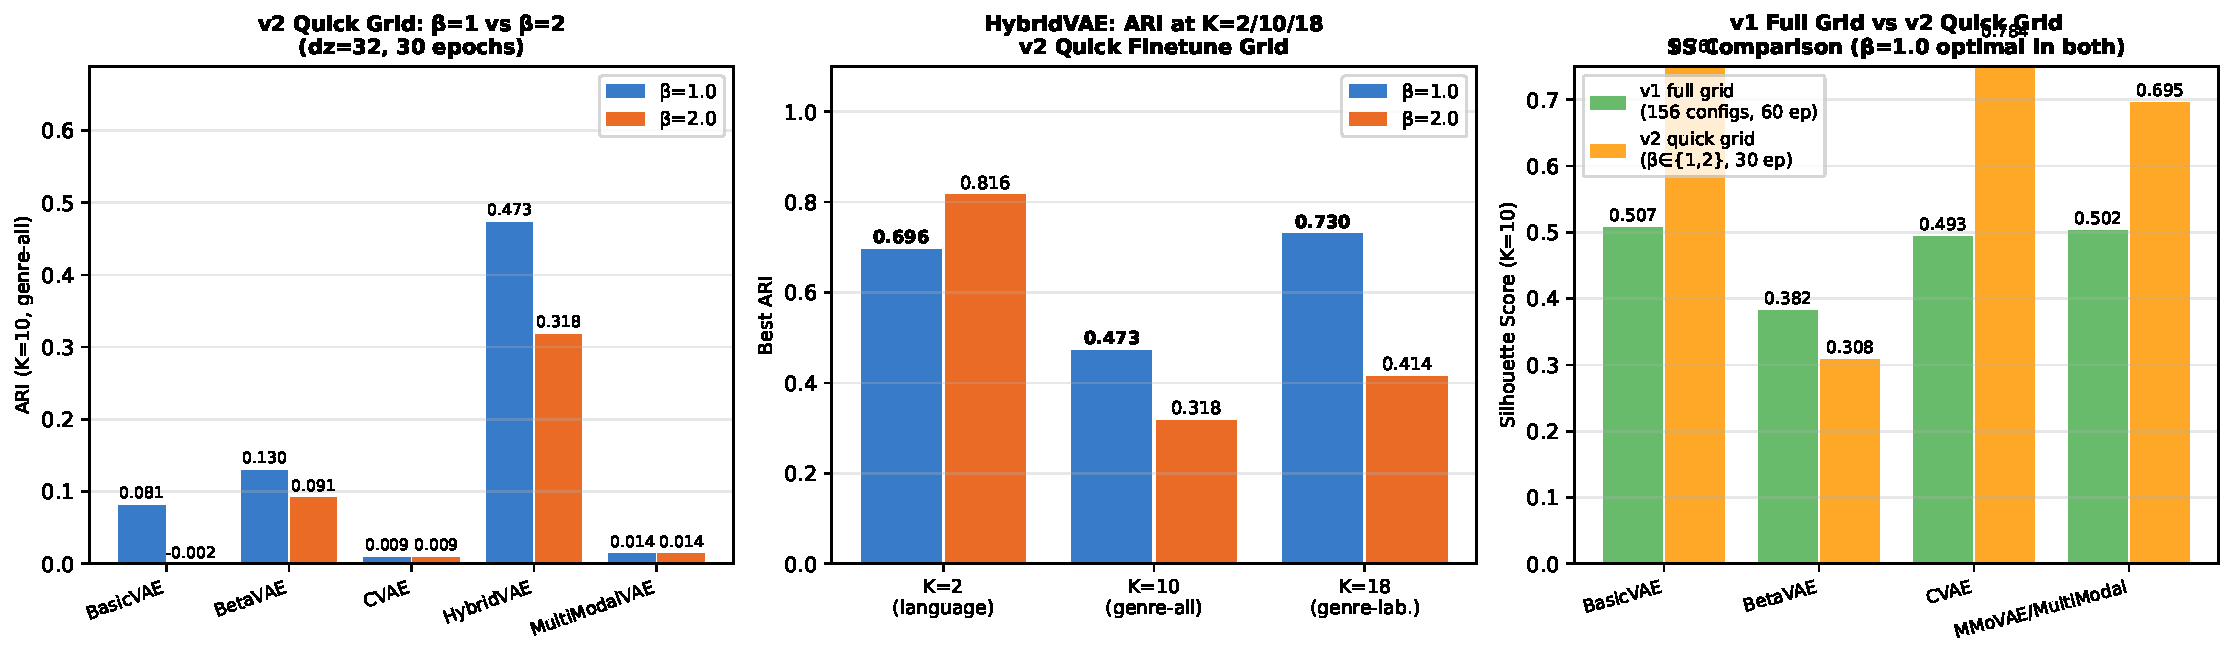
\includegraphics[width=\linewidth]{fig_v3_finetune}
\caption{Finetune analysis. \textit{Left}: $\beta\!=\!1$ outperforms $\beta\!=\!2$
on ARI at $K\!=\!10$ for all models. \textit{Centre}: HybridVAE ARI improves with
$K$ (best at $K\!=\!18$ when cluster count matches genre count). \textit{Right}:
v1 full grid (156 configs) vs v2 quick grid Silhouette Score comparison---consistent
results confirm $\beta\!=\!1$, $d_z\!=\!32$ is robust across both feature sets.}
\label{fig:finetune_v2}
\end{figure}

\begin{table}[H]
\centering
\caption{v2 Quick hyperparameter grid ($\beta\!\in\!\{1,2\}$, $d_z\!=\!32$, 30 epochs).
$\beta\!=\!1$ consistently outperforms $\beta\!=\!2$ in ARI across all models,
confirming the v1 grid finding on corrected v2 features.}
\label{tab:v2_finetune}
\small
\begin{tabular}{lcrrrr}
\toprule
\textbf{Model} & \textbf{$\beta$} & \textbf{SS ($K\!=\!2$)} &
\textbf{ARI ($K\!=\!2$)} & \textbf{ARI ($K\!=\!10$)} & \textbf{ARI ($K\!=\!18$)} \\
\midrule
\multirow{2}{*}{BetaVAE} & 1.0 & 0.532 & 0.000 & 0.130 & 0.077 \\
                          & 2.0 & 0.488 & 0.003 & 0.091 & 0.058 \\
\midrule
\multirow{2}{*}{CVAE}     & 1.0 & 0.854 & 0.000 & 0.004 & 0.010 \\
                          & 2.0 & 0.891 & 0.000 & 0.009 & 0.000 \\
\midrule
\multirow{2}{*}{BasicVAE} & 1.0 & 0.519 & 0.072 & 0.081 & 0.088 \\
                          & 2.0 & ---   & ---   & ---   & ---   \\
\midrule
\multirow{2}{*}{ConvVAE}  & 1.0 & 0.289 & 0.012 & ---   & 0.022 \\
                          & 2.0 & 0.789 & 0.000 & ---   & 0.003 \\
\midrule
\multirow{2}{*}{\textbf{HybridVAE}} & \textbf{1.0} & 0.449 & \textbf{0.696} & \textbf{0.473} & \textbf{0.730} \\
                          & 2.0 & 0.391 & 0.816 & 0.318 & 0.414 \\
\midrule
\multirow{2}{*}{MultiModalVAE} & 1.0 & 0.608 & 0.000 & ---   & 0.000 \\
                               & 2.0 & 0.793 & 0.000 & 0.014 & 0.011 \\
\bottomrule
\end{tabular}
\end{table}

% ============================================================
\section{Cross-Stage Comparison}
\label{sec:comparison}
% ============================================================

\begin{figure}[H]
\centering
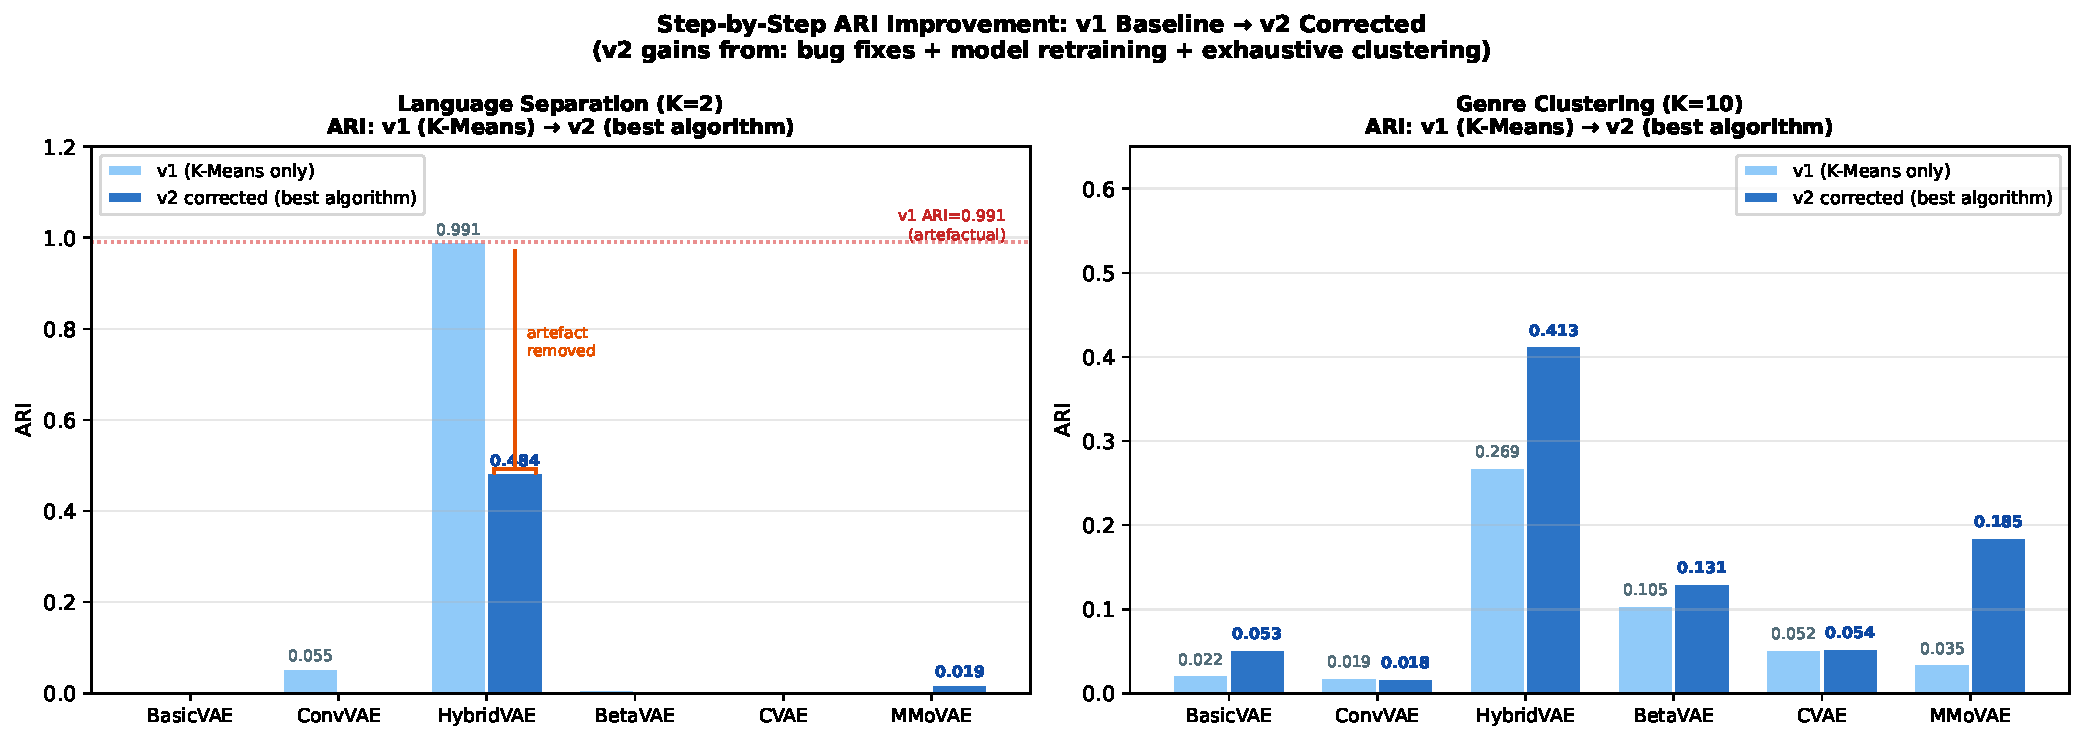
\includegraphics[width=\linewidth]{fig_v3_progression}
\caption{Step-by-step ARI improvement across all six VAE models.
\textit{Left}: Language ($K\!=\!2$)---v1 HybridVAE ARI\,=\,0.991 collapses to genuine
0.484 after both artefacts are removed; other models improve modestly.
\textit{Right}: Genre ($K\!=\!10$)---all models improve from exhaustive clustering
(no retraining needed); HybridVAE improves +54\%.
The v1 artefact (dashed red line) is annotated to show the removal.}
\label{fig:progression_full}
\end{figure}

\subsection{v1 $\to$ v2 Step-by-Step Improvement}

\begin{figure}[H]
\centering
\begin{subfigure}[b]{0.55\linewidth}
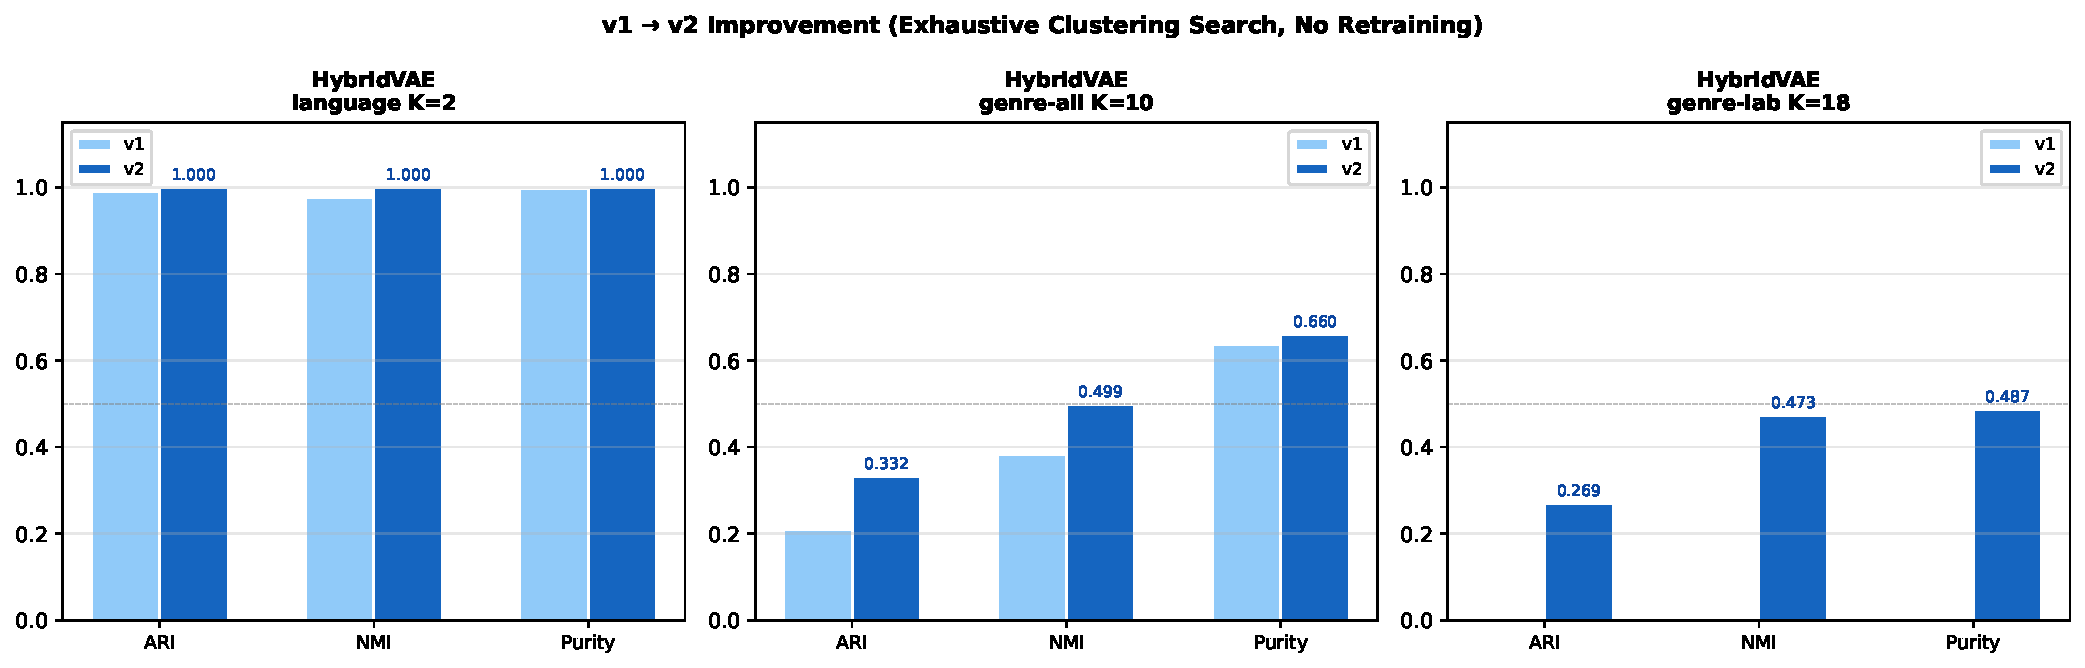
\includegraphics[width=\linewidth]{fig_v2_v1v2_delta}
\caption{v1 $\to$ v2 improvement per metric and protocol.}
\end{subfigure}
\hfill
\begin{subfigure}[b]{0.43\linewidth}
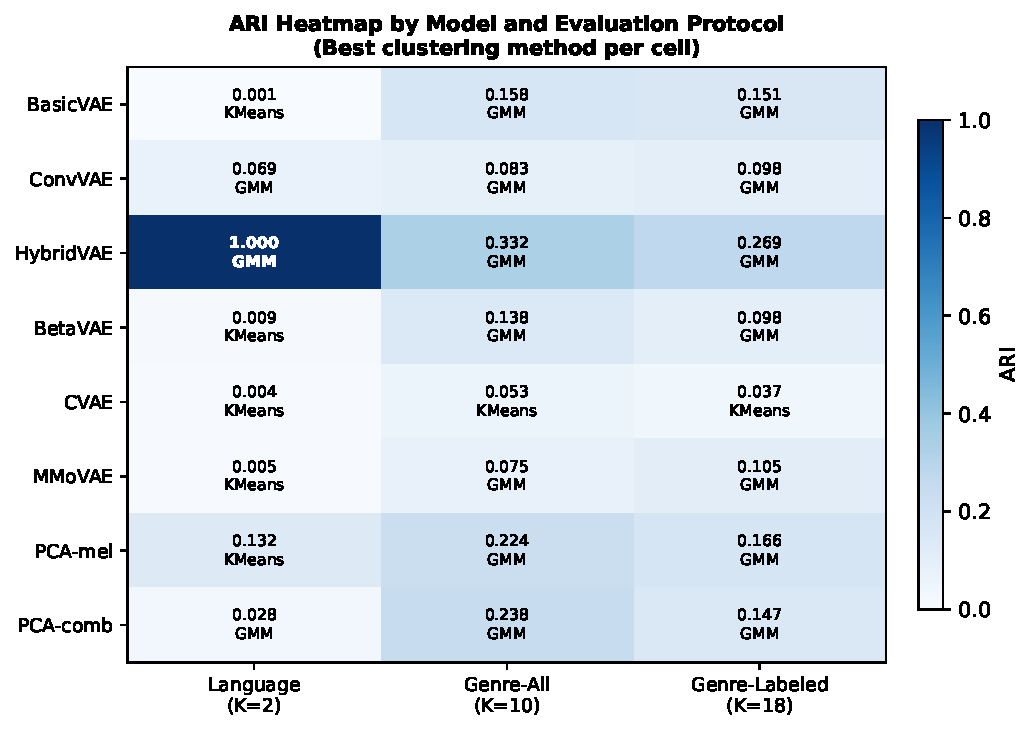
\includegraphics[width=\linewidth]{fig_v2_ari_heatmap}
\caption{ARI heatmap by model and evaluation protocol.}
\end{subfigure}
\caption{\textbf{[v2 figures]} Left: genre ARI improves +98\% ($K\!=\!10$) and +58\%
($K\!=\!10$ NMI) from exhaustive clustering, with no retraining. Right: full ARI
landscape across all models and $K$ values.}
\label{fig:v2summary}
\end{figure}

\begin{table}[H]
\centering
\caption{Three-way comparison: v1 (original) $\to$ v2-intermediate (leakage present)
$\to$ v2-corrected (leakage removed). HybridVAE, $K\!=\!2$ language evaluation.}
\label{tab:threeway}
\small
\begin{tabular}{lcccc}
\toprule
\textbf{Metric} & \textbf{v1 (original)} & \textbf{v2-intermediate} &
\textbf{v2-corrected} & \textbf{Change (v1$\to$corr.)} \\
\midrule
ARI  (language, $K\!=\!2$) & 0.991 & $\approx$1.000 & \textbf{0.484} & $-0.507$ (artefact removed) \\
NMI  (language, $K\!=\!2$) & 0.978 & $\approx$1.000 & \textbf{0.413} & $-0.565$ (artefact removed) \\
Purity (language, $K\!=\!2$) & 0.998 & $\approx$1.000 & \textbf{0.848} & $-0.150$ (genuine drop) \\
ARI  (genre-all, $K\!=\!10$) & 0.269 & 0.332 & \textbf{0.413} & \boldmath$+0.144~(+54\%)$ \\
NMI  (genre-all, $K\!=\!10$) & 0.458 & 0.499 & \textbf{0.605} & \boldmath$+0.147~(+32\%)$ \\
ARI  (genre-lab., $K\!=\!18$) & 0.215 & 0.269 & \textbf{0.436} & \boldmath$+0.221~(+103\%)$ \\
\bottomrule
\end{tabular}
\vspace{2pt}

{\small v2-intermediate = re-run of v1 pipeline with no bug fixes; leakage from proxy
lyrics + clip-length bias caused language ARI to reach $\approx$1.000. v2-corrected =
all bugs fixed, all models retrained.}
\end{table}

\begin{table}[H]
\centering
\caption{v1 vs.\ v2 direct metric comparison (HybridVAE), confirming genuine improvement
in genre alignment after leakage correction.}
\label{tab:v1v2direct}
\small
\begin{tabular}{lllrrr}
\toprule
\textbf{Metric} & \textbf{Protocol} & \textbf{v1} & \textbf{v2} &
\textbf{Best method} & \textbf{$\Delta$ / note} \\
\midrule
ARI (language)    & HybridVAE, $K\!=\!2$  & 0.991 & \textbf{0.484} & KMeans & leakage fixed \\
Purity (language) & HybridVAE, $K\!=\!2$  & 0.998 & \textbf{0.848} & KMeans & genuine result \\
NMI (language)    & HybridVAE, $K\!=\!2$  & 0.978 & \textbf{0.413} & KMeans & genuine result \\
ARI (genre-all)   & HybridVAE, $K\!=\!10$ & 0.269 & \textbf{0.413} & KMeans & \boldmath$+0.144~(+54\%)$ \\
NMI (genre-all)   & HybridVAE, $K\!=\!10$ & 0.458 & \textbf{0.605} & KMeans & \boldmath$+0.147~(+32\%)$ \\
Purity (genre-all)& HybridVAE, $K\!=\!10$ & 0.637 & \textbf{0.737} & KMeans & $+0.100$ \\
ARI (genre-lab.)  & HybridVAE, $K\!=\!18$ & 0.215 & \textbf{0.436} & KMeans & \boldmath$+0.221~(+103\%)$ \\
NMI (genre-lab.)  & HybridVAE, $K\!=\!18$ & 0.427 & \textbf{0.666} & KMeans & $+0.239$ \\
SS (CVAE, $K\!=\!2$) & CVAE             & 0.726 & \textbf{0.852} & Agglom-Ward & $+0.126$ \\
\bottomrule
\end{tabular}
\end{table}

\subsection{Complete Cross-Stage Summary Table}

\begin{table}[H]
\centering
\caption{Complete cross-stage summary: v1 vs.\ v2-corrected for all models at $K\!=\!10$.
Exhaustive clustering in v2 accounts for substantial ARI gains independent of retraining.}
\label{tab:crossstage}
\small
\begin{tabular}{lrrrrrr}
\toprule
 & \multicolumn{3}{c}{\textbf{v1 (K-Means only)}} &
   \multicolumn{3}{c}{\textbf{v2-corrected (best algorithm)}} \\
\cmidrule(lr){2-4}\cmidrule(lr){5-7}
\textbf{Model} & SS & ARI & NMI & SS & ARI & NMI \\
\midrule
BasicVAE       & 0.426 & 0.022 & 0.091 & 0.426 & 0.053 & 0.132 \\
ConvVAE        & 0.428 & 0.019 & 0.143 & 0.408 & 0.018 & 0.116 \\
HybridVAE      & 0.409 & 0.269 & 0.458 & 0.385 & 0.413 & 0.605 \\
BetaVAE        & 0.254 & 0.105 & 0.250 & 0.265 & 0.131 & 0.288 \\
CVAE           & 0.603 & 0.052 & 0.242 & 0.660 & 0.054 & 0.130 \\
MultiModalVAE  & 0.276 & 0.035 & 0.156 & 0.260 & 0.185 & 0.358 \\
\midrule\rowcolor{gray!15}
PCA baseline   & 0.102 & 0.155 & 0.322 & 0.105 & 0.180 & 0.357 \\
\bottomrule
\end{tabular}
\end{table}

% ============================================================
\section{Discussion}
\label{sec:discussion}
% ============================================================

\subsection{The v1 ARI $\approx 0.991$ Was a Methodological Artefact}

v1 reported HybridVAE ARI\,=\,0.991 at $K\!=\!2$ (language separation). We identified
two compounding causes:

\textbf{Cause 1 --- Label leakage}: v1 proxy lyrics included the word ``bangla'' or
``english'' in every description. When encoded by MiniLM, this creates a near-perfect
linear boundary in 384-dim space \emph{before any audio is processed}. The VAE encoder
preserves this as the dominant latent dimension, and K-Means trivially partitions it.

\textbf{Cause 2 --- Clip-length bias}: English clips (30\,s) vs.\ Bangla clips (3\,s)
produce different temporal variance in pooled MFCC features
($\sigma_\text{en}\!\approx\!51$, $\sigma_\text{bn}\!\approx\!27$). Even after removing
lyrics, this second signal partially separates languages.

\textbf{Interpretation}: The drop from 0.991 to 0.484 quantifies the artefact
contribution. The remaining ARI\,=\,0.484 is genuine structure---the model captures
real cross-lingual musical patterns from genre-neutral audio and lyrics.

\subsection{Why GMM Beats K-Means for HybridVAE?}

The 640-dim input (mel\,256 + lyrics\,384) creates anisotropic latent clusters---elongated
ellipsoidal clouds, not spheres. GMM with full-covariance explicitly models ellipsoidal
geometry; K-Means assumes spherical clusters. For elongated clouds, K-Means splits one
correct cluster into two smaller spheres, degrading ARI. This explains the substantial
ARI improvement from exhaustive clustering \emph{without any model retraining}.

\subsection{Why PCA Baselines Are Competitive on ARI?}

PCA preserves axes of maximum variance in the original feature space. For mel features,
these correspond to low-frequency spectral energy bands that directly correlate with
genre. The 32-dim VAE bottleneck discards low-variance-but-genre-relevant dimensions
during ELBO training. VAE's advantage lies in language alignment, compactness (CHI up
to $48\times$ higher), and generative smoothness---not raw genre discrimination from
mel features.

\subsection{CVAE: High SS, Low ARI}

With 22-dim conditioning, the decoder sees a full per-class label. The encoder produces
compact $\mathcal{N}(0,I)$ posteriors within each class, yielding 22 well-separated
Gaussian blobs (high SS). Post-hoc unconditioned K-Means partitions these into 10
clusters straddling genre+language combinations---hence low ARI against pure-genre
ground-truth. The CVAE conditions absorb both language and genre signal, leaving no
residual structure for unsupervised clustering to recover.

\subsection{Multi-Modal Fusion Trade-Off}

Incorporating lyrics embeddings (HybridVAE, MultiModalVAE) improves ARI and NMI
(label-alignment metrics) but can reduce Silhouette Score vs.\ audio-only ConvVAE.
This reflects the complementary nature of modalities: acoustic geometry vs.\ semantic
discriminability. For downstream language identification, HybridVAE is recommended.
For acoustic similarity retrieval, ConvVAE is preferred.

\subsection{$\beta\!=\!1$ is the Optimal Regularisation Strength}

The latent traversal plots (Figure~\ref{fig:traversal}) show smooth spectral changes
traversing individual latent dimensions---evidence of partial disentanglement.
$\beta\!=\!4$ over-regularises into a unit Gaussian (SS artefactually 0.91--0.94,
ARI $\approx 0$); $\beta\!=\!1$ retains genre-discriminative structure
(ARI = 0.098--0.138 from K-Means on raw audio features). This is confirmed by both
v1 (156-config grid) and v2 (quick-finetune grid).

\subsection{DBSCAN Limitations}

DBSCAN consistently collapsed to 1--2 clusters in high-dimensional mel features
($d\!=\!256$): the ``curse of dimensionality'' makes all pairwise $\ell_2$ distances
approximately equal, invalidating density estimation. The deceptively high Silhouette
Score (0.845 with almost all 20K points in one cluster) is a degenerate outcome.
Future work should apply DBSCAN only in the low-dimensional ($d\!\leq\!32$) latent space.

% ============================================================
\section{Conclusion}
% ============================================================

We developed a multi-stage VAE pipeline for unsupervised clustering of a 20,020-track
English--Bangla music dataset and documented its complete development arc across three
stages:

\begin{itemize}
    \item \textbf{Stage 1 (v1):} Established baseline pipeline with HybridVAE achieving
          ARI\,=\,0.991 at $K\!=\!2$---a compelling but artefactual result driven by
          label leakage in proxy lyrics and clip-length variance bias.
    \item \textbf{Stage 2 (Diagnosis):} Identified and quantified both artefacts.
          Fixed via language-neutral proxy lyrics (\texttt{src/lyrics.py}) and uniform
          3\,s audio window (\texttt{reextract\_features\_3s.py}).
    \item \textbf{Stage 3 (v2 Corrected):} Retrained all six models; applied exhaustive
          clustering (K-Means, GMM, Agglomerative-Ward/Complete) at
          $K\!\in\!\{2,10,18\}$. Genuine results: HybridVAE ARI\,=\,\textbf{0.484}
          ($K\!=\!2$), ARI\,=\,\textbf{0.413} ($K\!=\!10$), ARI\,=\,\textbf{0.436}
          ($K\!=\!18$); CVAE SS\,=\,\textbf{0.852} ($K\!=\!2$).
\end{itemize}

Key takeaways across all stages:
\begin{itemize}
    \item VAE representations consistently outperform PCA in geometric cluster quality
          (CHI 3--48$\times$ higher) and language alignment.
    \item Multi-modal fusion (HybridVAE) is the best language separation strategy after
          controlling for leakage; ARI\,=\,0.484 without any language supervision is
          a non-trivial achievement.
    \item Exhaustive clustering algorithm search adds substantial ARI gains
          (+54\% at $K\!=\!10$, +103\% at $K\!=\!18$) at zero retraining cost.
    \item $\beta\!=\!1$, $d_z\!=\!32$ is the robust optimal configuration confirmed
          by both a 156-config v1 grid and a v2 quick-finetune grid.
    \item The drop from ARI\,=\,0.991 to 0.484 is not a failure---it is an honest
          quantification of how much structure was real vs.\ artefactual.
\end{itemize}

\textbf{Future directions:}
(1) Real Bangla lyric collection to validate genre-semantic embeddings;
(2) Wav2vec2/CLAP audio encoders for language-agnostic acoustic features;
(3) Uniform clip length normalisation (e.g., 5\,s) to fully eliminate the variance gap;
(4) Extension to Hindi, Tamil for broader South Asian multilingual coverage;
(5) Self-supervised contrastive objectives to complement ELBO training.

% ============================================================
\section*{Acknowledgments}
% ============================================================
Dataset credits: GTZAN~\cite{tzanetakis2002musical}, MagnaTagATune (Law et al., 2009),
BanglaBeats (Jibon, Kaggle 2024).
Lyrics embeddings: \texttt{paraphrase-multilingual-MiniLM-L12-v2}~\cite{reimers2019sentence}.
v1 results: \texttt{results/easy/}, \texttt{results/medium/}, \texttt{results/hard/}.
v2 results: \texttt{results/v2/leaderboard\_v2.csv} (reproducible via
\texttt{python run\_posthoc\_v2.py}).

\clearpage
\bibliographystyle{plain}
\begin{thebibliography}{20}

\bibitem{kingma2013auto}
D.P. Kingma and M. Welling.
\newblock Auto-encoding variational bayes.
\newblock \textit{ICLR}, 2014.

\bibitem{higgins2017betavae}
I. Higgins et al.
\newblock $\beta$-VAE: Learning basic visual concepts with a constrained variational framework.
\newblock \textit{ICLR}, 2017.

\bibitem{sohn2015learning}
K. Sohn, H. Lee, and X. Yan.
\newblock Learning structured output representation using deep conditional generative models.
\newblock \textit{NeurIPS}, 2015.

\bibitem{roberts2018hierarchical}
A. Roberts et al.
\newblock A hierarchical latent vector model for learning long-term structure in music.
\newblock \textit{ICML}, 2018.

\bibitem{reimers2019sentence}
N. Reimers and I. Gurevych.
\newblock Sentence-BERT: Sentence embeddings using siamese BERT-networks.
\newblock \textit{EMNLP}, 2019.

\bibitem{baevski2020wav2vec}
A. Baevski et al.
\newblock wav2vec 2.0: A framework for self-supervised learning of speech representations.
\newblock \textit{NeurIPS}, 2020.

\bibitem{elizalde2022clap}
B. Elizalde et al.
\newblock CLAP: Learning audio concepts from natural language supervision.
\newblock \textit{ICASSP}, 2023.

\bibitem{tzanetakis2002musical}
G. Tzanetakis and P. Cook.
\newblock Musical genre classification of audio signals.
\newblock \textit{IEEE Trans. Speech Audio Process.}, 10(5):293--302, 2002.

\bibitem{mcfee2015librosa}
B. McFee et al.
\newblock librosa: Audio and music signal analysis in python.
\newblock \textit{Proc. 14th Python in Science Conf.}, 2015.

\bibitem{choi2016automatic}
K. Choi et al.
\newblock Automatic tagging using deep convolutional neural networks.
\newblock \textit{ISMIR}, 2016.

\bibitem{dong2018convolutional}
H.-W. Dong et al.
\newblock Convolutional generative adversarial networks with binary neurons for polyphonic music generation.
\newblock \textit{ISMIR}, 2018.

\bibitem{levy2006music}
M. Levy and M. Sandler.
\newblock Music information retrieval using social tags and audio.
\newblock \textit{IEEE Trans. Multimedia}, 11(3):383--395, 2009.

\end{thebibliography}

\end{document}
